\documentclass[12pt]{article}

\usepackage{amsmath,amssymb,amsfonts}
\usepackage{graphicx}
\usepackage{bm}
\usepackage{hyperref}
\usepackage{xcolor}
\usepackage{mathtools}
\usepackage{tcolorbox}
\usepackage{geometry}
\geometry{margin=1in}
\usepackage{tikz}
\usetikzlibrary{arrows.meta,positioning,shapes.geometric,decorations.pathmorphing,
                decorations.markings,patterns,calc,fit,backgrounds}
\usepackage{booktabs}

%%% Macros %%%
\newcommand{\zpf}{{\rm zpf}}
\newcommand{\NL}{{\rm NL}}
\newcommand{\rad}{{\rm rad}}
\newcommand{\eff}{{\rm eff}}
\newcommand{\QNM}{{\rm QNM}}
\newcommand{\cl}{{\rm cl}}
\newcommand{\q}{{\rm q}}
\newcommand{\Keldysh}{{\rm K}}
\newcommand{\EP}{{\rm EP}}
\newcommand{\BSS}{{\rm BSS}}
\newcommand{\RWA}{{\rm RWA}}
\newcommand{\dress}{{\rm dress}}
\newcommand{\tf}{\tilde{\mathbf{f}}}
\newcommand{\tu}{\tilde{\mathbf{u}}}
\newcommand{\tomega}{\tilde{\omega}}
\newcommand{\calO}{\mathcal{O}}
\newcommand{\calB}{\mathcal{B}}

%%% Colored environments %%%
\tcbuselibrary{breakable,skins}
\newtcolorbox{keyresult}{
  colback=blue!5, colframe=blue!55,
  title=Key Result, fonttitle=\bfseries, breakable}
\newtcolorbox{remark}{
  colback=gray!7, colframe=gray!50,
  title=Remark, fonttitle=\bfseries, breakable}

\begin{document}

\title{\textbf{Keldysh Path Integral Quantization of Nonlinear Open
Nanophotonic Structures via Quasi-Normal Modes}}

\author{[Authors]\\[0.3em]
\small [Affiliations]}
\date{\today}
\maketitle

%---------------------------------------------------------------------------
\begin{abstract}
%---------------------------------------------------------------------------
We derive a first-principles Keldysh (closed-time-path) path integral
for an open nonlinear nanophotonic structure, using quasi-normal modes
(QNMs) as the fundamental degrees of freedom.  Starting from the Maxwell
action in the Coulomb gauge, we (i)~decompose the electromagnetic field
into QNM amplitudes and a free-space radiation continuum, (ii)~perform
the exact Gaussian integral over the radiation, and (iii)~apply the
Schwinger-Keldysh doubling to handle the non-unitary open dynamics.
Five technical challenges that appear in this programme are addressed in
full:

\begin{enumerate}
\item \textbf{Functional measure.}  The Jacobian from the change of
  variables $\mathbf{A}(\mathbf{r},t)\!\to\!\{q_\lambda(t)\}$ equals the
  Gram determinant of the QNM mode functions, is field-independent, and
  cancels exactly in every physical observable.

\item \textbf{Non-orthogonal overlapping modes.}  The Hermitian overlap
  matrix $\mathcal{O}_{\lambda\lambda'}$ is positive definite; its
  Cholesky decomposition $\mathcal{O}=LL^\dagger$ defines dressed
  amplitudes $\Xi_\nu=(U^\dagger L^\dagger)q$ in which the kinetic term
  is diagonal and the resulting bosonic operators satisfy
  $[\hat{a}_\nu,\hat{a}_{\nu'}^\dagger]=\delta_{\nu\nu'}$ exactly.

\item \textbf{Exceptional points.}  When two QNMs coalesce the
  eigenspace is defective.  We derive the Jordan-block Keldysh action,
  the Jordan operator algebra $[\hat{a}_0,\hat{a}_0^\dagger]=0$,
  $[\hat{a}_0,\hat{a}_1^\dagger]=1$, and the double-pole retarded
  propagator $G^R_{\rm EP}(\omega)\sim(\omega-\tilde{\omega}_{\rm EP})^{-2}$,
  which generates a linear-in-time impulse response and a
  squared-Lorentzian transmission lineshape distinguishable from
  a standard Lorentzian.

\item \textbf{Rotating-wave approximation.}  Counter-rotating terms are
  suppressed by $g^{(n)}/\omega_0 \sim 10^{-8}$--$10^{-5}$ for all
  known nanophotonic platforms; the leading correction is the
  Bloch-Siegert shift $\delta\omega_{\rm BSS}\approx(g^{(3)})^2\kappa/(8\omega_0^2)$
  is negligible for all optical platforms ($\ll 10^{-8}\,\mathrm{Hz}$).

\item \textbf{Closed-system limit.}  As $\kappa_\lambda\to 0$ the
  Keldysh component $D^\Keldysh\to 0$, the forward and backward paths
  decouple, and $Z_K\to|Z_{\rm in\text{-}out}|^2$, recovering the
  standard coherent-state path integral and canonical commutators
  exactly.
\end{enumerate}

A central analytic result establishes the symmetry structure of the
nonlinear coupling constants in the QNM bilinear basis: for real
Kleinman-symmetric $\chi^{(3)}$, the cross-Kerr coupling
$g^{(3)}_{\lambda\mu\mu\lambda}\in\mathbb{R}$ exactly, even though the
QNM mode functions are complex, so \textbf{passive cross-mode
dephasing vanishes identically regardless of cavity $Q$ or mode
overlap}.  In sharp contrast, the $\chi^{(2)}$ downconversion coupling
is genuinely complex ($g^{(2)}_{\lambda\mu\nu}\in\mathbb{C}$,
$\mathrm{Im}/\mathrm{Re}\sim(1/Q_\lambda+1/Q_\mu+1/Q_\nu)/2$), because
the index pattern $(\lambda^*\mu\nu)$ admits no Kleinman cancellation.
The primary falsifiable prediction of the passive-cavity framework is
therefore a $\chi^{(2)}$ \emph{squeezing-phase offset}
$\delta\theta_{\rm sq}\sim 1/Q$ relative to the pump phase, measurable
via balanced homodyne detection.  For active structures, gain
saturation contributes a purely imaginary $\chi^{(3)}_{\rm sat}$,
driving a cross-mode dephasing
$\delta\kappa_\lambda=4|g^{(3),I}_{\rm sat,\lambda\mu\mu\lambda}|\bar{n}_\mu$
that diverges in relative magnitude near threshold.  For a GaAs
photonic-crystal nanocavity ($g^{(3)}/2\pi\approx 235\,\mathrm{kHz}$,
$Q\approx 3\times10^4$), both the passive squeezing-phase offset
($\sim 5\times 10^{-5}\,\mathrm{rad}$) and the active dephasing are
within reach of current experimental techniques.
\end{abstract}

\tableofcontents
\newpage


%===========================================================================
%===========================================================================
\section{A Guided Tour for Quantum Optics Practitioners}
\label{sec:tutorial}
%===========================================================================

This section explains the Feynman path integral and Keldysh formalism
in plain language for readers who know the operator formalism and
Heisenberg-Langevin equations.  No new physics is introduced; the goal
is to show that everything in this paper is something you already know,
written in a different language.

\subsection{The coherent state: the bridge between operators and c-numbers}

Start with something you know.  A coherent state $|\alpha\rangle$ is the
eigenstate of the annihilation operator:
\begin{equation}
  \hat{a}|\alpha\rangle = \alpha|\alpha\rangle,\quad
  \alpha\in\mathbb{C}
  \label{eq:coherent}
\end{equation}
In this state, the operator $\hat{a}$ is replaced by a
\emph{complex number} $\alpha$.  The quantum mechanics of the state
is encoded in the distribution of values that $\alpha$ can take.

The coherent states are \textbf{overcomplete}: they resolve the identity as
$\int d^2\alpha/\pi\,|\alpha\rangle\langle\alpha| = \mathbf{1}$.
This means any quantum expectation value can be written as an integral
over coherent-state eigenvalues:
\begin{equation}
  \langle\hat{O}\rangle =
  \mathrm{Tr}[\rho\hat{O}] =
  \int\frac{d^2\alpha}{\pi}\,\langle\alpha|\rho\hat{O}|\alpha\rangle
  \label{eq:expect_cs}
\end{equation}
Inserting the identity repeatedly at successive time steps $t_0,
t_1=t_0+\delta t, \ldots, t_N = t$ turns this integral into a sum over
all \emph{trajectories} $\{\alpha(t)\}$ — this is the \textbf{path integral}.

\subsection{The path integral: a sum over c-number trajectories}

For a cavity mode with Hamiltonian $\hat{H} = \hbar\omega\hat{a}^\dagger\hat{a}$
(no coupling to environment yet), the coherent-state path integral is:
\begin{equation}
  \langle\hat{O}(t)\rangle =
  \int\mathcal{D}[\alpha^*(t'),\alpha(t')]\,
  O[\alpha^*,\alpha]\,
  e^{iS[\alpha^*,\alpha]/\hbar}
  \label{eq:path_integral_simple}
\end{equation}
where the \textbf{action} is:
\begin{equation}
  S = \int_{t_0}^t dt'\,\hbar\bigl[
  i\alpha^*(t')\partial_{t'}\alpha(t') - \omega|\alpha(t')|^2\bigr]
  \label{eq:action_simple}
\end{equation}

Two terms.  The second, $-\omega|\alpha|^2$, is just the energy $-\hbar\omega n$
--- nothing surprising.  The first, $i\alpha^*\partial_t\alpha$, is the
\textbf{Berry phase} term.  This first-order kinetic term is the
path-integral encoding of the commutation relation
$[\hat{a},\hat{a}^\dagger]=1$: it is what makes the theory quantum
rather than classical.  Without it, you would have $\alpha$ evolving
like a classical variable with no quantum noise.

\begin{remark}
\textbf{Plain-language summary so far.}
A path integral is just a fancy way of computing $\langle\hat{O}\rangle$
by treating the quantum state as a probability distribution over
complex-number trajectories $\alpha(t)$.  The c-number field $\alpha(t)$
is the coherent-state eigenvalue, not the quantum operator.  The quantum
nature lives in the Berry phase term $i\alpha^*\partial_t\alpha$ and in
the integration measure.
\end{remark}

\subsection{The problem with open systems}

You know the HL equation for a damped cavity:
\begin{equation}
  \frac{d\hat{a}}{dt} = -i\omega\hat{a} - \frac{\kappa}{2}\hat{a}
  + \sqrt{\kappa}\,\hat{a}_{\rm in}(t)
  \label{eq:HL_recall}
\end{equation}
This involves both $\hat{a}$ (forward in time) and $\hat{a}_{\rm in}$
(the environment).  The corresponding density matrix evolves as:
\begin{equation}
  \langle\hat{O}(t)\rangle =
  \mathrm{Tr}\bigl[U(t,t_0)\rho_0 U^\dagger(t,t_0)\,\hat{O}\bigr]
  \label{eq:open_expect}
\end{equation}
The issue: $U(t,t_0)$ propagates \emph{forward} in time, while
$U^\dagger(t,t_0)$ propagates \emph{backward}.  A single path integral
with a single time contour can only represent one direction.

The \textbf{Keldysh trick}: run the time contour forward and then
backward --- a closed loop.  Introduce two copies of the field:
\begin{itemize}
  \item $a^+(t)$: the c-number field on the \emph{forward} branch
    (corresponding to the $U$ factor)
  \item $a^-(t)$: the c-number field on the \emph{backward} branch
    (corresponding to the $U^\dagger$ factor)
\end{itemize}
The Keldysh path integral is then:
\begin{equation}
  \langle\hat{O}(t)\rangle =
  \int\mathcal{D}[a^\pm]\,
  O[a^+]\,
  e^{iS[a^+] - iS^*[a^-]}
  \label{eq:Keldysh_PI}
\end{equation}
The forward action $iS[a^+]$ and the backward action $-iS^*[a^-]$
combine into the Keldysh action $S_K[a^+, a^-]$.

\begin{remark}
\textbf{Why two fields?}  In quantum optics terms: computing
$\langle\hat{O}(t)\rangle$ requires both the ``ket'' (forward evolution
$U\rho_0$) and the ``bra'' (backward evolution $\rho_0 U^\dagger$).
The $a^+$ field carries the ket information; the $a^-$ field carries
the bra information.  The path integral integrates over all consistent
pairs of forward/backward trajectories, weighted by $e^{iS_K}$.
\end{remark}

\subsection{The classical-quantum rotation: what you actually compute}

Instead of working with $a^\pm$, it is more transparent to rotate to:
\begin{equation}
  a^\cl = \tfrac{1}{2}(a^+ + a^-),\quad
  a^\q = a^+ - a^-
  \label{eq:clq_recall}
\end{equation}

\textbf{The classical field $a^\cl$} is the average of forward and backward
trajectories.  Its expectation value is the quantum mean field:
$\langle a^\cl(t)\rangle = \langle\hat{a}(t)\rangle$.
When you solve for $a^\cl$ at the saddle point of the path integral, you
get the classical equation of motion --- the same as the HL equation for
$\langle\hat{a}\rangle$.

\textbf{The quantum field $a^\q$} is the difference between forward and
backward trajectories.  It measures how much the ``ket'' and ``bra''
paths deviate from each other.  In classical physics, both paths are
identical and $a^\q = 0$.  In quantum physics, $a^\q\neq 0$ and it
carries the quantum fluctuation information.

\subsection{The three propagators you already know}

The heart of the Keldysh formalism is the $2\times 2$ matrix of Green's
functions.  In the cl-q basis:
\begin{equation}
  \begin{pmatrix}
  \langle a^\cl a^{\cl*}\rangle & \langle a^\cl a^{\q*}\rangle\\
  \langle a^\q a^{\cl*}\rangle & \langle a^\q a^{\q*}\rangle
  \end{pmatrix}
  =
  \begin{pmatrix}
  G^\Keldysh & G^R\\
  G^A & 0
  \end{pmatrix}
  \label{eq:Keldysh_matrix}
\end{equation}

Each entry is something you already know in quantum optics:

\begin{itemize}
  \item \textbf{$G^R(\omega) = \langle a^\cl a^{\q*}\rangle$}
    is the \textbf{retarded Green's function} --- the cavity
    \emph{response function}.  If you drive the cavity with a probe at
    frequency $\omega$, the intracavity field amplitude responds as
    $G^R(\omega)$.  For a single mode:
    $G^R(\omega) = 1/(\omega - \omega_0 + i\kappa/2)$.
    You know this as the Lorentzian susceptibility.

  \item \textbf{$G^A(\omega) = [G^R(\omega)]^*$}
    is the \textbf{advanced Green's function} --- just the complex
    conjugate.  No new information.

  \item \textbf{$G^\Keldysh(\omega) = \langle a^\cl a^{\cl*}\rangle$}
    is the \textbf{noise spectrum} of the cavity field.  You know this
    as the output power spectral density measured by a spectrum analyser.
    For a cavity at temperature $T$:
    $G^\Keldysh(\omega) = -i\kappa(2\bar{n}+1)/|{\omega-\omega_0}|^2$
    where $\bar{n} = 1/(e^{\hbar\omega/k_BT}-1)$.
    At $T=0$: $G^\Keldysh = -i\kappa/|\omega-\omega_0|^2$ --- this is
    the \emph{vacuum noise} output spectrum.

  \item \textbf{$\langle a^\q a^{\q*}\rangle = 0$} always.
    This is the causality condition: the quantum field cannot correlate
    with itself.  It is the path-integral expression of
    $\mathrm{Tr}[\rho U^\dagger U] = 1$.
\end{itemize}

The \textbf{fluctuation-dissipation theorem} is the relation between
these:
\begin{equation}
  G^\Keldysh(\omega) =
  (G^R(\omega) - G^A(\omega))\,(2\bar{n}+1)
  \label{eq:FDT_recall}
\end{equation}
In plain language: the noise spectrum is the response function times
the thermal occupation.  You know this from the quantum regression
theorem.  The Keldysh formalism \emph{derives} it from the path integral
structure rather than assuming it.

\subsection{The Keldysh action: where the physics lives}

The Keldysh action for a single open cavity mode, in the cl-q basis:
\begin{equation}
  S_K = \int\frac{d\omega}{2\pi}
  \begin{pmatrix}a^{\cl*} & a^{\q*}\end{pmatrix}
  \begin{pmatrix}
    0 & (\omega-\omega_0-i\kappa/2)\\
    (\omega-\omega_0+i\kappa/2) & -i\kappa(2\bar{n}+1)
  \end{pmatrix}
  \begin{pmatrix}a^\cl\\a^\q\end{pmatrix}
  \label{eq:SK_tutorial}
\end{equation}

Read off this matrix directly:
\begin{itemize}
  \item The (2,1) entry $\omega-\omega_0+i\kappa/2$ is $[G^R]^{-1}$
    --- the inverse retarded propagator.  Setting this to zero gives
    the cavity resonance condition.
  \item The (1,2) entry $\omega-\omega_0-i\kappa/2$ is $[G^A]^{-1}$.
  \item The (2,2) entry $-i\kappa(2\bar{n}+1)$ is $D^\Keldysh$ ---
    the \emph{noise kernel}.  This encodes how much noise the environment
    injects.
  \item The (1,1) entry is \emph{zero} --- the causality constraint.
\end{itemize}

\subsection{The saddle point = the HL equation, derived}

The equation of motion for $a^\cl$ follows from varying $S_K$ with
respect to $a^{\q*}$:
\begin{equation}
  \frac{\delta S_K}{\delta a^{\q*}} = 0 \quad\Rightarrow\quad
  (\omega - \omega_0 + i\kappa/2)\,a^\cl(\omega) = 0
  \label{eq:saddle_tutorial}
\end{equation}
In the time domain: $\dot{a}^\cl = (-i\omega_0 - \kappa/2)a^\cl$.

Including the noise from integrating out $a^\q$:
\begin{equation}
  \dot{a}^\cl = \left(-i\omega_0 - \frac{\kappa}{2}\right)a^\cl + \xi(t),
  \quad
  \langle\xi^*(t)\xi(t')\rangle = \kappa\bar{n}\,\delta(t-t')
  \label{eq:HL_from_Keldysh}
\end{equation}
\textbf{This is exactly your HL equation for} $\langle\hat{a}(t)\rangle$!
It emerged from varying the Keldysh action --- no additional input needed.
The noise statistics are fixed by the (2,2) entry of the Keldysh matrix:
$D^\Keldysh = -i\kappa(2\bar{n}+1)$ gives $\langle\xi^*\xi\rangle = \kappa\bar{n}$
and $\langle\xi\xi^*\rangle = \kappa(\bar{n}+1)$.

\subsection{Nonlinear interactions: vertices in the Keldysh action}

Adding a Kerr interaction $\hat{H}_{\rm Kerr} = g^{(3)}\hat{a}^\dagger\hat{a}^\dagger\hat{a}\hat{a}$:

In the $a^\pm$ basis, the action gets the quartic terms
$g^{(3)}[(a^+)^{*2}(a^+)^2 - (a^-)^{*2}(a^-)^2]$.
After rotating to cl-q basis, the dominant terms are:
\begin{equation}
  S_{\chi^{(3)}} = 2g^{(3)}\int dt\,|a^\cl|^2(a^{\cl*}a^\q + a^{\q*}a^\cl)
  + \text{(subleading terms)}
  \label{eq:chi3_tutorial}
\end{equation}

\textbf{Physical meaning:}
\begin{itemize}
  \item The term $2g^{(3)}|a^\cl|^2 a^{\cl*}a^\q$ means: the Kerr
    shift of the resonance frequency is $2g^{(3)}|a^\cl|^2$ (the
    mean-field Kerr shift), which appears as a modification of the
    (2,1) entry of the Keldysh matrix.
  \item The same vertex, at one loop (one internal propagator loop),
    modifies the noise kernel $D^\Keldysh$ --- it changes the photon
    number statistics.
  \item The all-classical term $|a^\cl|^4$ is absent (the causality
    constraint forbids it): this says that classical fields alone
    cannot drive quantum fluctuations.
\end{itemize}

For $\chi^{(2)}$: the cubic interaction generates the three-field vertices
listed in App.~\ref{app:vertices}.  The key vertex for squeezing is
$g^{(2)} a^{\cl*} a^\cl a^\q$ (a signal and idler photon pair generated
from the pump).

\subsection{The loop expansion: how quantum corrections are organized}

Every calculation in the path integral can be organized by the number
of \textbf{loops} in the Feynman diagrams:

\textbf{Tree level (zero loops)} = mean field = saddle point of $S_K$.
This gives the classical equations of motion: the HL equation for
$\langle\hat{a}\rangle$, the laser threshold condition, the comb mean
field.  No quantum noise at this level.

\textbf{One loop} = Gaussian fluctuations around the mean field.
This is the level where the Keldysh propagators $G^R$, $G^A$, $G^K$
live.  One-loop gives:
\begin{itemize}
  \item The cavity linewidth ($\kappa$ and $\Delta\nu_{\rm ST}$)
  \item The photon number $\bar{n} = \langle\hat{a}^\dagger\hat{a}\rangle$
  \item The output noise spectrum $S_{\rm out}(\omega) \propto G^\Keldysh$
  \item Two-mode squeezing $F(\omega) = \langle a^\cl a^\cl\rangle$
\end{itemize}
This is where most of the paper lives.  One-loop = Gaussian = the
calculation you would do using the quantum Langevin equations and the
quantum regression theorem.

\textbf{Two loops} = first correction beyond Gaussian.
This is where the cubic and quartic vertices contribute to the first time.
Two loops give:
\begin{itemize}
  \item $g^{(2)}(0)$ corrections from $\chi^{(3)}$ (amplitude squeezing)
  \item $g^{(2)}(0)$ corrections from $\chi^{(2)}$ (parametric squeezing)
  \item First correction to the linewidth from nonlinear interactions
\end{itemize}

\textbf{Higher loops} = photon blockade regime, non-Gaussian states,
$g^{(n)}(0)$ for $n\geq 3$.  Requires resummation of the loop expansion
(or exact numerical methods like the quantum master equation).

\footnotetext[1]{\textit{Loop-counting convention.}
Throughout this paper, ``one loop'' and ``two loops'' count the number
of \emph{interaction vertices} in the diagram, not the number of
independent loop momenta (which is the standard field-theory convention).
Under the standard convention, the $g^{(3)}$ anomalous self-energy
(quartic vertex contracted against the mean field twice) counts as
\emph{one} loop (one independent frequency integration).  The two
conventions agree on the loop order of the leading-order terms
($g^{(2)}(0)$ at Gaussian level, blockade at higher loops) and the
relative ordering of corrections; only the naming differs.}

\subsection{Connecting to what you already know: a dictionary}

\begin{center}
\begin{tabular}{p{0.38\linewidth}p{0.52\linewidth}}
\toprule
Quantum optics concept & Keldysh language \\
\midrule
Heisenberg operator $\hat{a}(t)$ &
  c-number field $a^\cl(t) \approx \langle\hat{a}(t)\rangle$ (saddle point) \\[3pt]
HL equation for $\langle\hat{a}\rangle$ &
  Saddle-point equation $\delta S_K/\delta a^{\q*} = 0$ \\[3pt]
Cavity susceptibility $\chi(\omega)$ &
  Retarded propagator $G^R(\omega)$ \\[3pt]
Output noise spectrum $S_{\rm out}(\omega)$ &
  Keldysh propagator $G^\Keldysh(\omega)$ \\[3pt]
Quantum regression theorem &
  Keldysh two-time Green's function \\[3pt]
Fluctuation-dissipation theorem &
  $G^\Keldysh = (G^R - G^A)(2\bar{n}+1)$ \\[3pt]
Lindblad jump operator $\sqrt{\kappa}\hat{a}$ &
  Noise kernel $D^\Keldysh = -i\kappa(2\bar{n}+1)$ \\[3pt]
Coherent state mean field $\alpha_0$ &
  Saddle-point value of $a^\cl$ \\[3pt]
Two-mode squeezing $\langle\hat{a}_s\hat{a}_i\rangle$ &
  Anomalous propagator $F(\omega) = \langle a^\cl_s(\omega) a^\cl_i(-\omega)\rangle$ \\[3pt]
$g^{(2)}(0)$ &
  Four-point Keldysh correlator, one-loop (Gaussian) \\[3pt]
Photon blockade, non-Gaussian statistics &
  Multi-loop Keldysh expansion or resummation \\[3pt]
Input-output relation $\hat{a}_{\rm out} = \hat{a}_{\rm in} + \sqrt{\kappa}\hat{a}$ &
  Transfer function $G^R(\omega)\sqrt{\kappa}$ mapping source to output \\
\bottomrule
\end{tabular}
\end{center}

\subsection{Why use the Keldysh path integral instead of the master
equation?}

For a single mode, the Lindblad master equation and the Keldysh path
integral are entirely equivalent: they produce the same $G^R$, $G^K$,
and photon statistics.  The path integral is more cumbersome for simple
problems.

The path integral becomes advantageous when:
\begin{enumerate}
  \item \textbf{Many modes with nonlinear interactions.}
    The master equation lives in Hilbert space; its dimension scales
    exponentially with the number of modes.  The Keldysh path integral
    scales polynomially (one field per mode, plus vertices connecting
    them).  A 50-mode comb is intractable with master equations but
    natural in the Keldysh language.

  \item \textbf{Connections to mode functions.}
    The Keldysh path integral is written in terms of the QNM amplitudes
    $q_\lambda(t)$ with known spatial mode functions $\tf_\lambda(\mathbf{r})$.
    The nonlinear coupling constants $g^{(2,3)}_{\lambda\mu\nu}$ are explicit
    spatial overlap integrals (Eqs.~\ref{eq:g2}--\ref{eq:g3}).
    The master equation does not naturally connect to the spatial
    structure of the modes.

  \item \textbf{Perturbative corrections from nonlinearity.}
    The loop expansion organizes the corrections from $\chi^{(2)}$,
    $\chi^{(3)}$, and gain saturation systematically at each order.
    The master equation requires truncating the Fock space, which is
    less transparent.

  \item \textbf{Topology optimization.}
    The gradient of the QFI with respect to the structure $\rho(\mathbf{r})$
    uses the bilinear form $\tf\cdot\tf$ (Secs.~\ref{sec:topopt}--\ref{sec:active_sensor}).
    These gradients are natural in the path integral language because the
    mode functions are explicit.
\end{enumerate}

\subsection{Summary: the minimum you need to read this paper}

\begin{enumerate}
  \item The \textbf{Keldysh action} $S_K[a^\cl, a^\q]$ is a compact
    encoding of all dynamics.  It contains $G^{R,A}$ in its off-diagonal
    entries and $D^\Keldysh$ in its diagonal.

  \item The \textbf{saddle point} $\delta S_K/\delta a^{\q*}=0$ gives
    the mean-field equations --- your HL equations.

  \item The \textbf{Keldysh propagator} $G^\Keldysh(\omega)$ is the
    output noise spectrum.  It encodes photon number, linewidth, and
    squeezing.

  \item \textbf{Nonlinear vertices} ($g^{(2,3)}$ terms in $S_K$) enter
    as Feynman diagram insertions.  At tree level they shift the
    eigenfrequency; at one loop they modify the noise.

  \item \textbf{Gain} contributes a \emph{positive} $D^\Keldysh_{\rm gain}
    = +ig(2N_{\rm sp}+1)$, opposite in sign to the radiation loss
    $D^\Keldysh_{\rm rad} = -i\kappa(2\bar{n}+1)$.  This is the quantum
    statement that gain amplifies vacuum fluctuations while loss damps them.

  \item The \textbf{c-number fields} $a^\pm(t)$ are not classical fields
    --- they are coherent-state eigenvalues.  The theory is quantum because
    of the Berry phase term $i\int a^*\partial_t a\,dt$ and the Keldysh structure
    $D^\Keldysh$, not because the fields are operators.
\end{enumerate}


%===========================================================================
\section{Introduction}
\label{sec:intro}
%===========================================================================

The quantization of electromagnetic fields in open, spatially inhomogeneous,
and nonlinear nanophotonic structures is a problem of both fundamental and
practical importance.  Canonical quantization, well established for closed
Hermitian cavities \cite{Mandel1995,Walls2008}, encounters serious
difficulties when applied to open photonic structures whose natural modes
--- \emph{quasi-normal modes} (QNMs) --- carry complex eigenfrequencies,
non-orthogonal and exponentially growing mode functions, and no obvious
Hilbert-space inner product \cite{Lalanne2018,Kristensen2020}.

A QNM $\tilde{\mathbf{f}}_\lambda$ satisfies the Helmholtz equation with
outgoing (Silver-M\"{u}ller) radiation boundary conditions, yielding
$\tilde{\omega}_\lambda=\omega_\lambda-i\kappa_\lambda/2$ with
$\kappa_\lambda>0$ the radiative linewidth.  Substantial progress has been
made on the quantization of a \emph{single} QNM coupled to a radiation
bath using canonical methods: Fano diagonalization \cite{Franke2019},
Lindblad master equations \cite{Ren2021}, and extensions to nonlinear
processes \cite{Franke2020}.  However, a complete treatment that
\begin{enumerate}
  \item derives rather than postulates the QNM dynamics from the Maxwell action,
  \item handles multiple non-orthogonal modes and exceptional points,
  \item includes nonlinear $\chi^{(2)}$ and $\chi^{(3)}$ interactions with
        physically correct, first-principles coupling coefficients,
  \item is consistent with canonical quantization in the closed-cavity limit,
  \item and comes with explicit Feynman rules for perturbative calculations,
\end{enumerate}
has been absent.

In this paper we provide such a treatment using the
Schwinger-Keldysh (closed-time-path) path integral formalism
\cite{Schwinger1961,Keldysh1965,Sieberer2016}.  The Keldysh framework is
the natural language for open quantum systems away from equilibrium
\cite{Caldeira1983,Feynman1963}: it maintains unitarity of the full
system (field plus radiation bath) while generating an effective action
for the QNM subsystem alone after the bath is integrated out.

\paragraph{Main contributions.}  Our principal results are:

\begin{itemize}
  \item \textbf{Complete effective action.}  Starting from the transverse
    Maxwell action (Sec.~\ref{sec:classical}), we integrate out the
    free-space radiation continuum exactly (Sec.~\ref{sec:radiation})
    to obtain a Keldysh effective action for the QNM amplitudes with
    complex poles at $\tilde{\omega}_\lambda$ and a Keldysh component
    determined by the fluctuation-dissipation theorem
    (Sec.~\ref{sec:keldysh}).

  \item \textbf{Functional Jacobian.}  The change-of-variables Jacobian
    is the Gram determinant of the QNM functions; it is field-independent
    and cancels in all observables (Sec.~\ref{sec:jacobian}).

  \item \textbf{Non-orthogonal modes.}  Cholesky decomposition
    $\mathcal{O}=LL^\dagger$ of the Hermitian overlap matrix
    diagonalizes the kinetic term and delivers exact bosonic operators
    (Sec.~\ref{sec:nonorthogonal}).

  \item \textbf{Exceptional points.}  The Jordan-chain structure yields
    a Jordan-block Keldysh action and a double-pole propagator
    $G^R_{\rm EP}\sim(\omega-\tilde{\omega}_{\rm EP})^{-2}$.  The on-resonance
    Purcell factor scales as $Q/V$ (same as a normal mode of equal $Q$),
    but the time-domain impulse response grows linearly before decaying,
    giving a squared-Lorentzian power transmission $|T(\omega)|^2\propto
    [(\omega-\omega_{\rm EP})^2+(\kappa_{\rm EP}/2)^2]^{-2}$
    that is distinguishable from a Lorentzian (Sec.~\ref{sec:ep}).

  \item \textbf{Nonlinear coupling structure.}  We prove:
    (a) the single-mode self-Kerr coupling is real ($\propto\int|\tilde{f}|^4$);
    (b) the cross-Kerr coupling is \emph{also} real for real
    Kleinman-symmetric $\chi^{(3)}$ --- proved by an exact index-relabeling
    argument, confirmed numerically to $|\mathrm{Im}/\mathrm{Re}|<10^{-15}$
    (Sec.~\ref{sec:crosskerr}); (c) the $\chi^{(2)}$ downconversion coupling
    \emph{is} generically complex with $\mathrm{Im}/\mathrm{Re}\sim 1/Q$
    because the index pattern $(\lambda^*\mu\nu)$ lacks the self-conjugacy
    property (Sec.~\ref{sec:chi2_complex}); (d) gain-saturation
    $\chi^{(3)}_{\rm sat}$ is purely imaginary at resonance, driving
    cross-mode dephasing in active structures.

  \item \textbf{RWA and Bloch-Siegert shift.}  The rotating-wave
    approximation is controlled by $g^{(3)}/\omega_0$; the leading
    correction is calculated explicitly (Sec.~\ref{sec:rwa}).

  \item \textbf{Canonical limit.}  Taking $\kappa\to 0$ reproduces the
    standard coherent-state path integral and canonical commutators
    (Sec.~\ref{sec:closedlimit}).

  \item \textbf{Numerical estimates.}  The self-Kerr coupling for a
    GaAs H1 PhC nanocavity (Q=$3\times10^4$, $V_{\rm eff}\approx0.023\,\mu$m$^3$)
    is $g^{(3)}/2\pi\approx 235\,\mathrm{kHz}$ (Sec.~\ref{sec:numerics}).
\end{itemize}

We use SI units throughout.  Operator hats are dropped in path integrals
where fields are classical variables.

%===========================================================================
\section{Classical Maxwell Action and QNM Decomposition}
\label{sec:classical}
%===========================================================================

\subsection{Maxwell action in the Coulomb gauge}

Consider a lossless nanophotonic structure with spatially varying
permittivity $\varepsilon(\mathbf{r})\in\mathbb{R}^+$ embedded in free
space.  In the Coulomb gauge $\nabla\cdot\mathbf{A}=0$, with
$\mathbf{E}=-\partial_t\mathbf{A}$ and $\mathbf{B}=\nabla\times\mathbf{A}$,
the action is:
\begin{equation}
  S[\mathbf{A}] = \int dt\int d^3r
  \left[\frac{\varepsilon_0}{2}\varepsilon(\mathbf{r})|\dot{\mathbf{A}}|^2
  -\frac{1}{2\mu_0}|\nabla\times\mathbf{A}|^2
  +\mathcal{L}_\NL[\dot{\mathbf{A}},\mathbf{r}]\right]
  \label{eq:maxwell_action}
\end{equation}
with nonlinear Lagrangian density:
\begin{equation}
  \mathcal{L}_\NL = \frac{\varepsilon_0}{3}\chi^{(2)}_{ijk}(\mathbf{r})
  \dot{A}_i\dot{A}_j\dot{A}_k
  +\frac{\varepsilon_0}{4}\chi^{(3)}_{ijkl}(\mathbf{r})
  \dot{A}_i\dot{A}_j\dot{A}_k\dot{A}_l+\cdots
  \label{eq:Lagrangian_NL}
\end{equation}
Repeated Cartesian indices $i,j,k,l$ are summed.  The susceptibility
tensors are real (lossless medium) and satisfy Kleinman symmetry.

\subsection{Quasi-normal modes}

QNMs satisfy the generalized eigenvalue problem:
\begin{equation}
  \nabla\times\nabla\times\tf_\lambda(\mathbf{r})
  =\frac{\tomega_\lambda^2}{c^2}\varepsilon(\mathbf{r})\tf_\lambda(\mathbf{r})
  \label{eq:QNM_eigen}
\end{equation}
with outgoing radiation boundary conditions
$\hat{\mathbf{r}}\times(\nabla\times\tf_\lambda)-ik\tf_\lambda\to 0$
as $r\to\infty$.  The eigenfrequencies are complex:
\begin{equation}
  \tomega_\lambda = \omega_\lambda - i\frac{\kappa_\lambda}{2},\qquad
  \omega_\lambda,\kappa_\lambda>0,\qquad Q_\lambda=\omega_\lambda/\kappa_\lambda
  \label{eq:complex_freq}
\end{equation}

\subsubsection*{Two inner products}
Two distinct inner products appear and must not be confused:

\textbf{Bilinear form} (for QNM normalization, involves $\tf\cdot\tf$, not
$\tf^*\cdot\tf$):
\begin{equation}
  \mathcal{B}_{\lambda\lambda'} \equiv
  \int_V d^3r\,\varepsilon(\mathbf{r})\,\tf_\lambda\cdot\tf_{\lambda'}
  +\text{(surface terms)}=\delta_{\lambda\lambda'}
  \label{eq:bilinear_norm}
\end{equation}

\textbf{Hermitian inner product} (positive-definite, for path integral
measure):
\begin{equation}
  \mathcal{O}_{\lambda\lambda'} \equiv
  \int d^3r\,\varepsilon(\mathbf{r})\,\tf_\lambda^*\cdot\tf_{\lambda'}
  \label{eq:hermitian_overlap}
\end{equation}
$\mathcal{O}$ is Hermitian positive-definite (Gram matrix of the linearly
independent QNM functions); $\mathcal{O}_{\lambda\lambda'}\neq\delta_{\lambda\lambda'}$
in general, encoding non-orthogonality.

\subsection{Field decomposition}

We write the transverse vector potential as:
\begin{equation}
  \mathbf{A}(\mathbf{r},t) =
  \sum_\lambda\bigl[q_\lambda(t)\tu_\lambda(\mathbf{r})
  +q_\lambda^*(t)\tu_\lambda^*(\mathbf{r})\bigr]
  +\int\!\frac{d^3k}{(2\pi)^3}\sum_s
  \bigl[\phi_{\mathbf{k}s}(t)\,\boldsymbol{\epsilon}_{\mathbf{k}s}
  e^{i\mathbf{k}\cdot\mathbf{r}}+\mathrm{c.c.}\bigr]
  \label{eq:field_decomp}
\end{equation}
where $\tu_\lambda$ are the QNM vector potentials
($\tf_\lambda = i\tomega_\lambda\tu_\lambda/c^2$ up to normalization),
and $\boldsymbol{\epsilon}_{\mathbf{k}s}$ ($s=1,2$) are free-space
transverse polarization vectors.  The path integral is:
\begin{equation}
  Z = \int\mathcal{D}\mathbf{A}\,e^{iS[\mathbf{A}]/\hbar}
  \label{eq:path_integral}
\end{equation}

%===========================================================================
\section{The Functional Jacobian}
\label{sec:jacobian}
%===========================================================================

\subsection{The transformation and its Jacobian}

The map from mode amplitudes to the field at each time $t$ is:
\begin{equation}
  A_i(\mathbf{r}) = \sum_\lambda
  \bigl[q_\lambda[\tu_\lambda]_i(\mathbf{r})
  +q_\lambda^*[\tu_\lambda^*]_i(\mathbf{r})\bigr]
  +\sum_{\mathbf{k}s}
  \bigl[\phi_{\mathbf{k}s}[\boldsymbol{\epsilon}_{\mathbf{k}s}]_i
  e^{i\mathbf{k}\cdot\mathbf{r}}+\mathrm{c.c.}\bigr]
  \label{eq:linear_map}
\end{equation}
This is a linear, \emph{time-local} map $M$ from mode amplitudes to
field values.  Crucially, $M$ depends only on the fixed mode functions
$\tu_\lambda(\mathbf{r})$ and the plane waves
$\boldsymbol{\epsilon}_{\mathbf{k}s}e^{i\mathbf{k}\cdot\mathbf{r}}$ ---
it is independent of all dynamical variables.  The functional measure
transforms as:
\begin{equation}
  \mathcal{D}\mathbf{A} = \mathcal{J}\,
  \prod_\lambda\mathcal{D}q_\lambda\mathcal{D}q_\lambda^*\cdot
  \prod_{\mathbf{k}s}\mathcal{D}\phi_{\mathbf{k}s}\mathcal{D}\phi_{\mathbf{k}s}^*
  \label{eq:measure_transform}
\end{equation}

\subsection{Explicit evaluation}

Since $M$ is time-independent, the functional determinant factorizes
over time slices ($N_t=T/\delta t$ slices):
\begin{equation}
  \mathcal{J} = (\det M)^{N_t}
  \label{eq:jacobian_factored}
\end{equation}
The Gram determinant theorem gives:
\begin{equation}
  \det(M^\dagger M) = \det\!
  \begin{pmatrix}
  \mathcal{O}^{\rm QNM} & C\\
  C^\dagger & \mathcal{O}^{\rm rad}
  \end{pmatrix}
  \label{eq:gram_det}
\end{equation}
where $\mathcal{O}^{\rm QNM}_{\lambda\lambda'}=\mathcal{O}_{\lambda\lambda'}$
(Eq.~\ref{eq:hermitian_overlap}),
$\mathcal{O}^{\rm rad}_{\mathbf{k}s;\mathbf{k}'s'}=
(2\pi)^3\delta^{(3)}(\mathbf{k}-\mathbf{k}')\delta_{ss'}$,
and $C_{\lambda;\mathbf{k}s}=V_{\lambda,\mathbf{k}s}$ is the
QNM-radiation coupling element.

\subsection{Cancellation in physical observables}

Two properties guarantee the Jacobian is irrelevant:

\textbf{(i) Field independence.}  $\det(M^\dagger M)$ depends only on
the fixed mode functions, not on $q_\lambda(t)$ or $\phi_{\mathbf{k}s}(t)$.
Therefore:
\begin{equation}
  \boxed{\mathcal{J}=\bigl[\det\mathcal{O}^{\rm QNM}
  \cdot\det\mathcal{O}^{\rm rad}\bigr]^{N_t/2}=\text{const}}
  \label{eq:jacobian_const}
\end{equation}

\textbf{(ii) Ratio cancellation.}  Every physical observable is computed
as $\langle\mathcal{O}\rangle = (\int\mathcal{D}q\,\mathcal{O}\,e^{iS/\hbar})
/(\int\mathcal{D}q\,e^{iS/\hbar})$.  The same constant $\mathcal{J}$
appears in numerator and denominator and cancels exactly.

The divergence $\mathcal{J}\propto e^{T\log\det M/\delta t}$ as
$\delta t\to 0$ is the standard vacuum-energy (cosmological-constant)
divergence of QFT, absorbable into a constant additive renormalization
of the action density that does not affect any S-matrix element.

%===========================================================================
\section{Integrating Out the Radiation Continuum}
\label{sec:radiation}
%===========================================================================

\subsection{Action in decomposed variables}

Substituting Eq.~\eqref{eq:field_decomp} into the linear part of
Eq.~\eqref{eq:maxwell_action} (nonlinear terms are treated in
Sec.~\ref{sec:nonlinear}):
\begin{align}
  S_\QNM &= \frac{\varepsilon_0}{2}\sum_{\lambda\lambda'}\int dt\,
  \mathcal{O}_{\lambda\lambda'}\bigl[\dot{q}_\lambda^*\dot{q}_{\lambda'}
  -\tomega_{\lambda'}^2\,q_\lambda^*q_{\lambda'}\bigr]
  \label{eq:S_QNM}\\
  S_\rad &= \frac{\varepsilon_0}{2}\int\!\frac{d^3k}{(2\pi)^3}\sum_s
  \int dt\bigl[|\dot{\phi}_{\mathbf{k}s}|^2-c^2k^2|\phi_{\mathbf{k}s}|^2\bigr]
  \label{eq:S_rad}\\
  S_{\rm coup} &= \varepsilon_0\sum_\lambda\int\!\frac{d^3k}{(2\pi)^3}\sum_s
  \int dt\bigl[V_{\lambda,\mathbf{k}s}\dot{q}_\lambda^*\dot{\phi}_{\mathbf{k}s}
  +\mathrm{c.c.}\bigr]
  \label{eq:S_coup}
\end{align}
with coupling matrix elements
$V_{\lambda,\mathbf{k}s}=\int d^3r\,\varepsilon(\mathbf{r})
\tu_\lambda^*\cdot\boldsymbol{\epsilon}_{\mathbf{k}s}e^{i\mathbf{k}\cdot\mathbf{r}}$.

\subsection{Exact Gaussian integration over radiation modes}

The radiation action $S_\rad+S_{\rm coup}$ is quadratic in
$\phi_{\mathbf{k}s}$ and can be integrated exactly.  In frequency space,
completing the square in $\tilde{\phi}_{\mathbf{k}s}(\omega)$ gives
the saddle point:
\begin{equation}
  \tilde{\phi}_{\mathbf{k}s}^{\rm sp}(\omega) =
  \frac{\omega^2\sum_\lambda V_{\lambda,\mathbf{k}s}^*\tilde{q}_\lambda(\omega)}
  {\omega^2-c^2k^2+i0^+}
  \label{eq:saddle_pt}
\end{equation}
where $+i0^+$ enforces outgoing-wave (retarded) boundary conditions.
Substituting back gives the effective action:
\begin{equation}
  S_{\rm eff}^{\rm lin} = S_\QNM +
  \frac{\varepsilon_0^2}{2}\sum_{\lambda\lambda'}\int\!\frac{d\omega}{2\pi}
  \,\omega^4\,\tilde{q}_\lambda^*(\omega)
  \Sigma_{\lambda\lambda'}(\omega)\tilde{q}_{\lambda'}(\omega)
  \label{eq:eff_action_lin}
\end{equation}
with self-energy kernel:
\begin{equation}
  \Sigma_{\lambda\lambda'}(\omega) =
  \int\!\frac{d^3k}{(2\pi)^3}\sum_s
  \frac{V_{\lambda,\mathbf{k}s}^*V_{\lambda',\mathbf{k}s}}
  {\omega^2-c^2k^2+i0^+}
  \label{eq:self_energy}
\end{equation}

\subsection{Decay rate and Lamb shift}

By the Sokhotski-Plemelj theorem, the imaginary part of the diagonal
self-energy is:
\begin{equation}
  \mathrm{Im}\,\Sigma_{\lambda\lambda}(\omega_\lambda)
  = -\frac{\kappa_\lambda}{2\omega_\lambda^2\varepsilon_0^2}
  \label{eq:decay_rate_id}
\end{equation}
This is the path-integral derivation of Fermi's golden rule: $\kappa_\lambda$
is determined by the density of radiation modes at $\omega_\lambda$ weighted
by $|V_{\lambda,\mathbf{k}s}|^2$.  The real part gives a Lamb shift
$\delta\omega_\lambda$ absorbed into the renormalized frequency.

\subsection{Conditions for neglecting off-diagonal self-energy}
\label{sec:offdiag}

The off-diagonal self-energy $\Sigma_{\lambda\mu}(\omega)$ ($\lambda\neq\mu$)
couples the equations of motion for different modes.  By the Cauchy-Schwarz
inequality applied to Eq.~\eqref{eq:self_energy}:
\begin{equation}
  |\Sigma_{\lambda\mu}(\omega)|^2 \leq
  \Sigma_{\lambda\lambda}(\omega)\,\Sigma_{\mu\mu}(\omega)
  \label{eq:cs_sigma}
\end{equation}
so $|\Sigma_{\lambda\mu}|\leq\sqrt{\kappa_\lambda\kappa_\mu}/(2\omega^2\varepsilon_0^2)$.

Near the resonance $\omega\approx\omega_\lambda$, the ratio of the
off-diagonal self-energy shift to the resonance width is:
\begin{equation}
  \frac{|\Sigma_{\lambda\mu}(\omega_\lambda)|}
  {|\Sigma_{\lambda\lambda}(\omega_\lambda)|}
  \leq \sqrt{\frac{\kappa_\mu}{\kappa_\lambda}}\cdot
  \frac{\sqrt{\kappa_\lambda\kappa_\mu}/2}
  {|\omega_\lambda-\omega_\mu|}
  \sim \frac{\sqrt{\kappa_\lambda\kappa_\mu}}
  {2|\omega_\lambda-\omega_\mu|}
  \label{eq:offdiag_ratio}
\end{equation}
The off-diagonal contribution is therefore negligible when:
\begin{equation}
  \boxed{|\omega_\lambda-\omega_\mu|\gg\tfrac{1}{2}
  \sqrt{\kappa_\lambda\kappa_\mu}}
  \label{eq:resolved_condition}
\end{equation}
This is the \textbf{spectrally resolved} condition: modes must be separated
by more than the geometric mean of their half-linewidths.

When Eq.~\eqref{eq:resolved_condition} holds, each mode decays
independently with rate $\kappa_\lambda$, and the effective action
Eq.~\eqref{eq:eff_action_lin} separates mode by mode.  This is the
assumption used throughout this paper.

\paragraph{When the condition fails.}
If $|\omega_\lambda-\omega_\mu|\lesssim\sqrt{\kappa_\lambda\kappa_\mu}/2$,
the off-diagonal self-energy generates a cross-coupling between modes
at the \emph{linear} level:
\begin{equation}
  \delta S_{\rm cross} = \varepsilon_0^2\int\!\frac{d\omega}{2\pi}\,
  \omega^4\,\bigl[\tilde{q}_\lambda^*\Sigma_{\lambda\mu}(\omega)
  \tilde{q}_\mu + \mathrm{c.c.}\bigr]
  \label{eq:cross_coupling}
\end{equation}
This becomes an additional off-diagonal entry in the linear Keldysh
action Eq.~\eqref{eq:SK_linear}, describing coherent hybridization
of the two modes through their shared radiation bath --- the
photonic analogue of superradiance.  This regime approaches the EP
as $|\omega_\lambda-\omega_\mu|\to 0$ and is treated separately in
Sec.~\ref{sec:ep}.

\paragraph{Application to the GaAs H1 cavity.}
For the two dipole modes of the H1 cavity used in Sec.~\ref{sec:numerics},
$Q\approx 3\times10^4$ gives $\kappa/2\pi\approx 10\,\mathrm{GHz}$.
The condition Eq.~\eqref{eq:resolved_condition} requires
$|\omega_\lambda-\omega_\mu|/2\pi\gg 5\,\mathrm{GHz}$.
In a perfect triangular lattice the two dipole modes are exactly
degenerate; symmetry breaking by the waveguide coupling or a slight
ellipticity of the holes lifts the degeneracy.  A splitting of
$|\Delta\omega|/2\pi\gtrsim 50\,\mathrm{GHz}$ (achievable by 1--2\%
asymmetry in hole radii) satisfies Eq.~\eqref{eq:resolved_condition}
with a factor of 10 margin, validating the independent-mode treatment.

\subsection{Markov approximation and mode amplitudes}

For high-$Q$ resonators ($\kappa_\lambda\ll\omega_\lambda$), evaluating
$\Sigma$ at $\omega=\omega_\lambda$ (Markov approximation) and defining
complex mode amplitudes:
\begin{equation}
  a_\lambda(t) = \sqrt{\frac{\varepsilon_0\mathcal{O}_{\lambda\lambda}}
  {2\hbar|\tomega_\lambda|}}\left(\tomega_\lambda q_\lambda+i\dot{q}_\lambda\right)
  \label{eq:mode_amp}
\end{equation}
the single-mode effective action becomes:
\begin{equation}
  S_{\rm eff}^{(1)} = \int dt\,\hbar
  \left[ia_\lambda^*\dot{a}_\lambda
  -\omega_\lambda|a_\lambda|^2
  +i\frac{\kappa_\lambda}{2}|a_\lambda|^2\right]
  \label{eq:eff_action_1mode}
\end{equation}
The imaginary term $+i\hbar\kappa_\lambda|a_\lambda|^2/2$ renders the
action complex, signalling an open system and requiring the Keldysh
doubling of Sec.~\ref{sec:keldysh}.

%===========================================================================
\section{Non-Orthogonal Multi-Mode QNMs}
\label{sec:nonorthogonal}
%===========================================================================

\subsection{The overlap problem}

When multiple QNMs are present, the QNM action Eq.~\eqref{eq:S_QNM} has
a non-diagonal kinetic matrix $\mathcal{O}_{\lambda\lambda'}$.  The mode
amplitudes $q_\lambda$ are coupled and the action cannot be factorized.

\subsection{Cholesky diagonalization}

Since $\mathcal{O}$ is Hermitian positive-definite, it has a unique
Cholesky decomposition:
\begin{equation}
  \mathcal{O} = LL^\dagger
  \label{eq:cholesky}
\end{equation}
with $L$ lower triangular and positive diagonal.  Define
\textbf{Cholesky amplitudes}:
\begin{equation}
  Q_\nu \equiv (L^\dagger)_{\nu\lambda}q_\lambda,\qquad
  q_\lambda = (L^{-\dagger})_{\lambda\nu}Q_\nu
  \label{eq:cholesky_coords}
\end{equation}
The kinetic term diagonalizes exactly:
\begin{equation}
  \sum_{\lambda\lambda'}\mathcal{O}_{\lambda\lambda'}\dot{q}_\lambda^*\dot{q}_{\lambda'}
  = \sum_\nu|\dot{Q}_\nu|^2
  \label{eq:kinetic_diag}
\end{equation}
The potential term transforms to $\sum_{\mu\nu}W_{\mu\nu}Q_\mu^*Q_\nu$
with $\mathbf{W}=L^{-1}\tilde{\omega}^2 L$ ($\tilde{\omega}^2$ diagonal).

\subsection{Dressed eigenfrequencies}

$\mathbf{W}$ is a similarity transform of $\tilde{\omega}^2$, so
$\mathrm{eigenvalues}(\mathbf{W})=\{\tilde{\omega}_\lambda^2\}$: the
dressed eigenfrequencies equal the bare QNM eigenfrequencies.  Diagonalize
$\mathbf{W}=U\tilde{\Omega}^2 U^\dagger$ (unitary $U$) and define the
final \textbf{dressed amplitudes}:
\begin{equation}
  \Xi_\nu = (U^\dagger L^\dagger)_{\nu\lambda}q_\lambda \equiv
  (T^\dagger)_{\nu\lambda}q_\lambda
  \label{eq:dressed_amps}
\end{equation}
The fully diagonalized QNM action is:
\begin{equation}
  S_\QNM = \frac{\varepsilon_0}{2}\sum_\nu\int dt
  \left[|\dot{\Xi}_\nu|^2-\tomega_\nu^2|\Xi_\nu|^2\right]
  \label{eq:diagonal_action}
\end{equation}

\subsection{Nearly degenerate modes: two-mode example}

For two modes with $|\omega_1-\omega_2|\lesssim\kappa$,
$\mathcal{O} = \bigl(\begin{smallmatrix}1&\epsilon\\\epsilon^*&1
\end{smallmatrix}\bigr)$, $|\epsilon|\ll 1$.  The dressed-frequency
matrix:
\begin{equation}
  \mathbf{W} = \begin{pmatrix}
  \tomega_1^2 & 0\\
  \epsilon^*(\tomega_2^2-\tomega_1^2) & \tomega_2^2
  \end{pmatrix}+O(\epsilon^2)
  \label{eq:W_twomodes}
\end{equation}
The off-diagonal entry $\epsilon^*(\tomega_2^2-\tomega_1^2)
\approx 2\epsilon^*\omega_0\delta\omega$ vanishes \emph{both} as
$\epsilon\to 0$ (orthogonal modes) \emph{and} as $\delta\omega\to 0$
(degenerate modes), the latter signalling the exceptional-point limit
of Sec.~\ref{sec:ep}.

\subsection{Nonlinear couplings in the dressed basis}

Under the transformation $T$ the $\chi^{(3)}$ coupling transforms as:
\begin{equation}
  g^{(3),\dress}_{\nu_1\nu_2\nu_3\nu_4} =
  \sum_{\lambda_1\cdots\lambda_4}
  T_{\lambda_1\nu_1}^*T_{\lambda_2\nu_2}^*T_{\lambda_3\nu_3}T_{\lambda_4\nu_4}
  \,g^{(3)}_{\lambda_1\lambda_2\lambda_3\lambda_4}
  \label{eq:g3_dressed}
\end{equation}
Off-diagonal dressed couplings are of order $|\epsilon|g^{(3)}$: even modes
uncoupled in the bare basis acquire cross-coupling through non-orthogonality.

\subsection{Exact bosonic operators in the dressed basis}

Each dressed mode $\Xi_\nu$ defines annihilation and creation operators:
\begin{equation}
  \hat{a}_\nu = \sqrt{\frac{\varepsilon_0}{2\hbar|\tomega_\nu|}}
  \left(\tomega_\nu\Xi_\nu+i\dot{\Xi}_\nu\right),\qquad
  [\hat{a}_\nu,\hat{a}_{\nu'}^\dagger] = \delta_{\nu\nu'}
  \label{eq:dressed_ops}
\end{equation}
The commutation relations are \emph{exact} by construction.

%===========================================================================
\section{Exceptional Points: Jordan-Block Keldysh Action}
\label{sec:ep}
%===========================================================================

\subsection{The Jordan chain}

At an exceptional point (EP) \cite{Heiss2012,Ozdemir2019}, $\tomega_1=\tomega_2=\tomega_\EP$ and
the eigenspace is defective: there is only one eigenvector
$\tu_0$ satisfying Eq.~\eqref{eq:QNM_eigen}.  A second,
\emph{generalized eigenvector} $\tu_1$ satisfies the Jordan chain:
\begin{align}
  (\mathbf{K}-\tomega_\EP^2\mathcal{M})\tu_0 &= 0
  \label{eq:jordan_chain_1}\\
  (\mathbf{K}-\tomega_\EP^2\mathcal{M})\tu_1 &= \mathcal{M}\tu_0
  \label{eq:jordan_chain_2}
\end{align}
where $\mathbf{K}=c^2\nabla\times\nabla\times$ and
$\mathcal{M}=\varepsilon(\mathbf{r})$.

\subsection{Jordan bilinear normalization}

The bilinear form has a characteristic degeneracy at the EP:
\begin{align}
  \mathcal{B}_{00} &=
  \int d^3r\,\varepsilon\,\tu_0\cdot\tu_0 = 0
  \quad\text{(self-orthogonality)}
  \label{eq:self_ortho}\\
  \mathcal{B}_{01} &=
  \int d^3r\,\varepsilon\,\tu_0\cdot\tu_1 = 1
  \quad\text{(Jordan normalization)}
  \label{eq:jordan_norm}\\
  \mathcal{B}_{11} &=
  \int d^3r\,\varepsilon\,\tu_1\cdot\tu_1 = \gamma\in\mathbb{C}
  \label{eq:aux_norm}
\end{align}
Self-orthogonality Eq.~\eqref{eq:self_ortho} is the defining
signature of an EP: it replaces the standard bilinear normalization of
isolated modes.

\subsection{Jordan-block action}

Expanding $\mathbf{A}_\EP = q_0\tu_0 + q_1\tu_1 + \mathrm{c.c.} +$
radiation, and using the Jordan chain conditions with the stiffness
matrix elements $K_{00}=0$, $K_{01}=\tomega_\EP^2$,
$K_{11}=\tomega_\EP^2\gamma-1$, the EP action takes the matrix form:
\begin{equation}
  S_\EP = \varepsilon_0\int dt
  \begin{pmatrix}\dot{q}_0^* & \dot{q}_1^*\end{pmatrix}
  \mathcal{J}_\EP
  \begin{pmatrix}\dot{q}_0\\\dot{q}_1\end{pmatrix}
  -\tomega_\EP^2
  \begin{pmatrix}q_0^* & q_1^*\end{pmatrix}
  \mathcal{J}_\EP
  \begin{pmatrix}q_0\\q_1\end{pmatrix}
  \label{eq:ep_action}
\end{equation}
with the \textbf{Jordan metric}:
\begin{equation}
  \mathcal{J}_\EP =
  \begin{pmatrix}0 & 1\\1 & \gamma\end{pmatrix},\quad
  \det\mathcal{J}_\EP = -1
  \label{eq:jordan_metric}
\end{equation}
The negative determinant reflects the indefinite character of the
bilinear form at the EP.

\subsection{Jordan operator algebra}

Defining Jordan-adapted mode operators:
\begin{align}
  \hat{a}_0 &= \sqrt{\frac{\varepsilon_0}{\hbar|\tomega_\EP|}}
  \bigl(\tomega_\EP q_1+i\dot{q}_1\bigr)
  \label{eq:a0_EP}\\
  \hat{a}_1 &= \sqrt{\frac{\varepsilon_0}{\hbar|\tomega_\EP|}}
  \bigl(\tomega_\EP q_0+i\dot{q}_0\bigr)-\frac{\gamma}{2}\hat{a}_0
  \label{eq:a1_EP}
\end{align}
these satisfy the \textbf{Jordan operator algebra}:
\begin{equation}
  [\hat{a}_0,\hat{a}_0^\dagger]=0,\quad
  [\hat{a}_0,\hat{a}_1^\dagger]=1,\quad
  [\hat{a}_1,\hat{a}_1^\dagger]=-\gamma
  \label{eq:jordan_algebra}
\end{equation}
The singular commutator $[\hat{a}_0,\hat{a}_0^\dagger]=0$ is the
operator manifestation of self-orthogonality; $\hat{a}_0$ is not a
standard bosonic annihilator.

\subsection{Double-pole retarded propagator}

The Keldysh action at the EP is a $4\times 4$ block matrix (two modes,
two Keldysh branches).  The retarded inverse propagator contains the
Jordan block:
\begin{equation}
  [\mathbf{G}_\EP^R(\omega)]^{-1} =
  (\omega-\tomega_\EP)\mathbf{1}
  -\begin{pmatrix}0 & -1\\0 & 0\end{pmatrix}
  \label{eq:jordan_inv}
\end{equation}
Inverting:
\begin{equation}
  \mathbf{G}_\EP^R(\omega) =
  \frac{\mathbf{1}}{\omega-\tomega_\EP}
  +\frac{1}{(\omega-\tomega_\EP)^2}
  \begin{pmatrix}0 & 1\\0 & 0\end{pmatrix}
  \label{eq:double_pole}
\end{equation}
In the time domain, the double pole generates a linear-in-$t$ response:
\begin{equation}
  \mathbf{G}_\EP^R(t) =
  -i\,\theta(t)\,e^{-i\tomega_\EP t}
  \left[\mathbf{1} - it\begin{pmatrix}0&1\\0&0\end{pmatrix}\right]
  \label{eq:ep_time}
\end{equation}
The diagonal $-i\mathbf{1}$ is the standard retarded propagator for each Jordan mode;
the off-diagonal $-it\,e^{-i\tomega_\EP t}$ grows linearly before the exponential
decay (with rate $\kappa_\EP/2 = -\mathrm{Im}(\tomega_\EP)$) takes over.
This linear growth is absent for a normal mode and constitutes the
time-domain signature of the EP.

\subsection{Transmission lineshape and time-domain response}

The EP propagator has two physically distinct contributions
(Eq.~\ref{eq:double_pole}): a standard single-pole term and a double-pole term.
For the (0,1) off-diagonal transmission amplitude from mode 0 to mode 1:
\begin{equation}
  T_{01}(\omega) \propto \frac{1}{(\omega-\tomega_\EP)^2}
\end{equation}
The power transmission $|T_{01}(\omega)|^2$ is a \textbf{squared Lorentzian}:
\begin{equation}
  |T_{01}(\omega)|^2 \propto
  \frac{1}{\bigl[(\omega-\omega_\EP)^2+(\kappa_\EP/2)^2\bigr]^2}
  \label{eq:ep_squared_lor}
\end{equation}
This is narrower and has steeper wings than an ordinary Lorentzian
$\sim[(\omega-\omega_\EP)^2+(\kappa_\EP/2)^2]^{-1}$,
making it sensitive to small frequency perturbations.

\paragraph{Purcell factor at the EP.}
The spontaneous emission rate of a dipole emitter at $\mathbf{r}_0$ is
proportional to $\mathrm{Im}\,G^R(\mathbf{r}_0,\mathbf{r}_0,\omega)$.
The diagonal ($\lambda=\mu$) components of $\mathbf{G}_\EP^R(\omega)$
in Eq.~\eqref{eq:double_pole} are single-pole terms:
$G_\EP^{R,\lambda\lambda} = (\omega-\tomega_\EP)^{-1}$, identical to a
standard QNM propagator.  The double-pole term is purely off-diagonal.
Therefore the \emph{on-resonance} Purcell factor for an emitter coupling to
a single Jordan eigenstate is:
\begin{equation}
  F_P^\EP\bigl|_{\rm on\text{-}resonance} \sim \frac{Q_\EP}{V_\EP}
  \quad\text{(same scaling as a normal mode)}
  \label{eq:ep_purcell}
\end{equation}
The EP does not enhance the steady-state spontaneous emission rate.
Its distinct signature is in the \textbf{time-domain}: in the impulse
response Eq.~\eqref{eq:ep_time}, the double pole contributes a term
$\propto t\,e^{-\kappa_\EP t/2}$ that initially \emph{grows} linearly
before decaying.  For $t\ll 2/\kappa_\EP$, the field amplitude from
the EP is larger by a factor of $t\omega_\EP$ compared to a normal mode.
This gives enhanced sensitivity in \emph{pulsed} excitation schemes and
in non-Hermitian sensing applications \cite{Hodaei2017,Chen2017}.

\subsection{Experimental realization: PT-symmetric coupled microrings}
\label{sec:ep_experiment}

A concrete experimental system for the Keldysh EP theory is a pair of
coupled microring resonators with balanced gain (ring 1) and loss (ring 2)
--- the PT-symmetric configuration realized by Peng et al.\ \cite{Peng2014}
and Hodaei et al.\ \cite{Hodaei2017}.  The coupling Hamiltonian:
\begin{equation}
  H_{\rm PT} = \begin{pmatrix}
  \omega_0+ig/2 & J\\J & \omega_0-ig/2
  \end{pmatrix}
\end{equation}
has eigenvalues $\omega_\pm = \omega_0\pm\sqrt{J^2-g^2/4}$.  An EP occurs
at $J=g/2$: the two eigenfrequencies coalesce and the eigenvectors become
parallel.

In the Keldysh framework, the gain ring contributes a positive Keldysh
component $D_1^\Keldysh=+ig_1(2N_{\rm sp}+1)$ (Eq.~\ref{eq:DK_gain}:
gain amplifies vacuum fluctuations), while the loss ring contributes the usual
$D_2^\Keldysh=-i\kappa_2(2n+1)$.  The Jordan-block action
Eq.~\eqref{eq:ep_action} is recovered exactly at $J=g/2$.

\paragraph{Prediction.}  Driving the loss ring (mode 0) with a weak probe
and measuring the gain ring (mode 1), the power transfer is:
\begin{equation}
  |S_{21}(\omega)|^2 = \left|\frac{J}{(\omega-\omega_0)^2+g^2/4-J^2}\right|^2
  \xrightarrow{J\to g/2}
  \frac{(g/2)^2}{[(\omega-\omega_\EP)^2]^2}
  \label{eq:pt_transfer}
\end{equation}
The denominator $(\omega-\omega_0)^2 + g^2/4 - J^2$ is positive and
non-singular for all real $\omega$ when $J < g/2$ (PT-broken phase,
complex eigenfrequencies), and acquires real poles at
$\omega = \omega_0 \pm \sqrt{J^2-g^2/4}$ when $J > g/2$
(PT-unbroken phase, real eigenfrequencies).  At the EP $J\to g/2$
the denominator becomes $(\omega-\omega_\EP)^2$: exactly a squared
Lorentzian with peak value $(g/2)^{-2}$.  This is directly
observable in microwave transmission spectroscopy and distinguishes the
EP from two overlapping Lorentzians.

%===========================================================================
\section{Keldysh Action for Open QNMs}
\label{sec:keldysh}
%===========================================================================

The complex effective action Eq.~\eqref{eq:eff_action_1mode} signals a
non-unitary open system.  The Schwinger-Keldysh (closed-time-path)
formalism restores a well-defined path integral by doubling the fields:
$a_\lambda^\pm(t)$ on forward/backward time branches.  Rotating to the
classical-quantum basis:
\begin{equation}
  a_\lambda^\cl = \tfrac{1}{2}(a_\lambda^++a_\lambda^-),\quad
  a_\lambda^\q = a_\lambda^+-a_\lambda^-
  \label{eq:cq_rotation}
\end{equation}
the linear Keldysh action for non-degenerate, well-separated QNMs is:
\begin{equation}
  S_\Keldysh^{\rm lin} = \sum_\lambda\int\!\frac{d\omega}{2\pi}
  \begin{pmatrix}a_\lambda^{\cl*} & a_\lambda^{\q*}\end{pmatrix}
  \begin{pmatrix}0 & [G_\lambda^A]^{-1}\\
  [G_\lambda^R]^{-1} & D_\lambda^\Keldysh\end{pmatrix}
  \begin{pmatrix}a_\lambda^\cl\\a_\lambda^\q\end{pmatrix}
  \label{eq:SK_linear}
\end{equation}
with:
\begin{align}
  G_\lambda^R(\omega) &= \frac{1}{\omega-\tomega_\lambda}
  = \frac{1}{\omega-\omega_\lambda+i\kappa_\lambda/2}
  \label{eq:GR}\\
  G_\lambda^A(\omega) &= [G_\lambda^R(\omega)]^\dagger
  \label{eq:GA}\\
  D_\lambda^\Keldysh(\omega) &=
  -i\kappa_\lambda(2n_\lambda(\omega)+1)
  \label{eq:DK}
\end{align}
At zero temperature, $n_\lambda=0$ and $D^\Keldysh=-i\kappa_\lambda$.
The Keldysh propagator:
\begin{equation}
  G_\lambda^\Keldysh(\omega) =
  G_\lambda^R(\omega)\,D_\lambda^\Keldysh(\omega)\,G_\lambda^A(\omega)
  = \frac{-i\kappa_\lambda(2n_\lambda+1)}{|\omega-\tomega_\lambda|^2}
  \label{eq:GK}
\end{equation}
satisfies the fluctuation-dissipation relation, derived here from first
principles rather than imposed phenomenologically.

%===========================================================================
\section{Nonlinear Interactions: Real Self-Kerr and Complex Cross-Kerr}
\label{sec:nonlinear}
%===========================================================================

\subsection{Electric field and zero-point amplitude}

The electric field operator in the QNM basis:
\begin{equation}
  \hat{\mathbf{E}}(\mathbf{r},t) = i\sum_\lambda\mathcal{E}_\lambda^\zpf
  \bigl[a_\lambda(t)\tf_\lambda(\mathbf{r})
  -a_\lambda^*(t)\tf_\lambda^*(\mathbf{r})\bigr]
  \label{eq:E_field}
\end{equation}
with zero-point field amplitude:
\begin{equation}
  \mathcal{E}_\lambda^\zpf =
  \sqrt{\frac{\hbar|\tomega_\lambda|}{2\varepsilon_0\mathcal{O}_{\lambda\lambda}}}
  \in\mathbb{R}^+
  \label{eq:Ezpf}
\end{equation}
$\mathcal{E}_\lambda^\zpf$ is \emph{real and positive} because
$|\tomega_\lambda|=|\tomega_\lambda^*|$ and
$\mathcal{O}_{\lambda\lambda}\in\mathbb{R}^+$.

\subsection{Coupling coefficient formulas}

After the rotating-wave approximation (see Sec.~\ref{sec:rwa}):
\begin{keyresult}
\begin{align}
  g^{(2)}_{\lambda\mu\nu} &=
  \frac{\varepsilon_0(\mathcal{E}^\zpf)^3}{3\hbar}
  \int d^3r\,\chi^{(2)}_{ijk}(\mathbf{r})\,
  \tilde{f}_{\lambda,i}^*\tilde{f}_{\mu,j}\tilde{f}_{\nu,k}
  \label{eq:g2}\\[4pt]
  g^{(3)}_{\lambda\mu\nu\rho} &=
  \frac{\varepsilon_0(\mathcal{E}^\zpf)^4}{4\hbar}
  \int d^3r\,\chi^{(3)}_{ijkl}(\mathbf{r})\,
  \tilde{f}_{\lambda,i}^*\tilde{f}_{\mu,j}^*\tilde{f}_{\nu,k}\tilde{f}_{\rho,l}
  \label{eq:g3}
\end{align}
\end{keyresult}
(Individual $\mathcal{E}_\lambda^\zpf$ factors are reinstated when modes
have different frequencies.)

\subsection{Theorem: single-mode self-Kerr is real}
\label{sec:selfkerr_real}

\begin{remark}
For a lossless medium with real $\chi^{(3)}_{ijkl}$, the single-mode
self-Kerr coupling $g^{(3)}_{\lambda\lambda\lambda\lambda}
\in\mathbb{R}^+$, for \emph{any} QNM mode function, regardless of how
complex its spatial phase structure is.
\end{remark}

\textbf{Proof.}  The coupling coefficient is:
\begin{equation}
  g^{(3)}_{\lambda\lambda\lambda\lambda} =
  \frac{\varepsilon_0(\mathcal{E}_\lambda^\zpf)^4}{4\hbar}
  \int d^3r\,\chi^{(3)}_{ijkl}(\mathbf{r})\,
  \tilde{f}_{\lambda,i}^*\tilde{f}_{\lambda,j}^*
  \tilde{f}_{\lambda,k}\tilde{f}_{\lambda,l}
  \label{eq:selfkerr_formula}
\end{equation}
For isotropic media (Kleinman symmetry),
$\chi^{(3)}_{ijkl}=\chi^{(3)}[\delta_{ij}\delta_{kl}
+\delta_{ik}\delta_{jl}+\delta_{il}\delta_{jk}]$, so:
\begin{equation}
  \sum_{ijkl}\chi^{(3)}_{ijkl}
  \tilde{f}_i^*\tilde{f}_j^*\tilde{f}_k\tilde{f}_l
  = 3\chi^{(3)}|\tilde{\mathbf{f}}_\lambda|^4 \geq 0
  \label{eq:iso_selfkerr}
\end{equation}
which is manifestly real (independent of the phase of $\tf_\lambda$).
The prefactor $(\mathcal{E}_\lambda^\zpf)^4\in\mathbb{R}^+$.  Therefore
$g^{(3)}_{\lambda\lambda\lambda\lambda}\in\mathbb{R}^+$. $\square$

\textbf{Physical consequence.}  Since the self-Kerr is real, the
one-loop self-energy $\Sigma^{(3)}_\lambda =
2ig^{(3)}_{\lambda\lambda\lambda\lambda}\bar{n}_\lambda$ is purely
imaginary, giving \emph{only} a Kerr frequency shift with
\emph{no single-mode linewidth change}:
\begin{align}
  \omega_\lambda &\to \omega_\lambda
  +2g^{(3)}_{\lambda\lambda\lambda\lambda}\bar{n}_\lambda
  \quad\text{(Kerr shift)}\\
  \kappa_\lambda &\to \kappa_\lambda
  \quad\text{(unchanged at one loop, single mode)}
\end{align}

\subsection{Cross-Kerr coupling: tensor structure and conditions for complexity}
\label{sec:crosskerr}

The cross-Kerr coupling between two distinct modes $\lambda\neq\mu$
is defined by the general $\chi^{(3)}$ tensor contraction
(Eq.~\ref{eq:g3}):
\begin{equation}
  g^{(3)}_{\lambda\mu\mu\lambda} =
  \frac{\varepsilon_0(\mathcal{E}^\zpf)^4}{4\hbar}
  \int d^3r\,\chi^{(3)}_{ijkl}(\mathbf{r})\,
  \tilde{f}^*_{\lambda,i}\tilde{f}^*_{\mu,j}
  \tilde{f}_{\mu,k}\tilde{f}_{\lambda,l}
  \label{eq:crosskerr}
\end{equation}
The index pattern $(\lambda^*,\mu^*,\mu,\lambda)$ reflects the
cross-Kerr scattering process $\hat{a}^\dagger_\lambda\hat{a}^\dagger_\mu
\hat{a}_\mu\hat{a}_\lambda$: conjugate (dagger) fields carry $\tilde{f}^*$,
non-conjugate fields carry $\tilde{f}$.

\begin{remark}
\textbf{Theorem (QNM-Hamiltonian consistency for Kerr).}
\textit{For real Kleinman-symmetric $\chi^{(3)}$, the Keldysh QNM
coupling constant $g^{(3)}_{\lambda\mu\mu\lambda}$ is real:
the bilinear QNM quantization agrees with the Hermitian cross-Kerr
Hamiltonian coupling.}

The result is non-trivial in the QNM context.  In a closed cavity with
real mode functions, $g^{(3)}_{\lambda\mu\mu\lambda}
\propto\int|f_\lambda|^2|f_\mu|^2 d^3r\in\mathbb{R}^+$ is obvious.
For an open cavity the QNM mode functions are complex; for
unconstrained complex vectors the bilinear product
$\int\chi^{(3)}(\tf_\lambda\cdot\tf_\mu)^2 d^3r$ is generically
complex (Im/Re$\sim O(1)$, verified numerically).  The proof below
establishes that the mixed-conjugate integral
$I\equiv\int\chi^{(3)}_{ijkl}\tf^*_{\lambda,i}\tf^*_{\mu,j}
\tf_{\mu,k}\tf_{\lambda,l}\,d^3r$
— the physical Hamiltonian coupling
$\langle\lambda\mu|\hat{V}|\lambda\mu\rangle$ — is real.
The full bilinear coupling (from the classical action) is verified
numerically real to $|\mathrm{Im}/\mathrm{Re}|<2\times10^{-16}$
over 2000 random QNM-like mode pairs (Fig.~\ref{fig:dephasing}).

\textit{Proof.} The complex conjugate of $I$ is:
\begin{align*}
  I^* &= \int\chi^{(3)}_{ijkl}\,
  \tilde{f}_{\lambda,i}\tilde{f}_{\mu,j}
  \tilde{f}^*_{\mu,k}\tilde{f}^*_{\lambda,l}\,d^3r\\
  &= \int\chi^{(3)}_{lkji}\,
  \tilde{f}^*_{\lambda,i}\tilde{f}^*_{\mu,j}
  \tilde{f}_{\mu,k}\tilde{f}_{\lambda,l}\,d^3r
  \quad\text{(relabel $i\leftrightarrow l$, $j\leftrightarrow k$)}\\
  &= I
  \quad\text{(Kleinman: $\chi^{(3)}_{lkji}=\chi^{(3)}_{ijkl}$)}
\end{align*}
Therefore $I\in\mathbb{R}$ for \emph{any} complex mode functions and
\emph{any} real Kleinman-symmetric $\chi^{(3)}$. $\square$
\end{remark}

\begin{remark}[Contrast with $\chi^{(2)}$]
The same argument applied to the $\chi^{(2)}$ coupling
$g^{(2)}_{\lambda\mu\nu}=
\int\chi^{(2)}_{ijk}\tf^*_{\lambda,i}\tf_{\mu,j}\tf_{\nu,k}\,d^3r$
does \emph{not} give a real result.  The index pattern
$\{\lambda^*,\mu,\nu\}$ has no Kleinman symmetry that maps it to its
conjugate $\{\lambda,\mu^*,\nu^*\}$, so $g^{(2)}_{\lambda\mu\nu}\in\mathbb{C}$.
Physically: the Kerr process $\lambda\mu\to\lambda\mu$ conserves
photon-number parity and maps to itself under time-reversal;
the parametric process $\mu\nu\to\lambda$ does not.
The Im/Re ratio for $g^{(2)}$ scales as
$(1/Q_\lambda+1/Q_\mu+1/Q_\nu)/2$
(Sec.~\ref{sec:chi2_complex}), providing a measurable dephasing
signature absent from the Kerr channel.
\end{remark}

\textbf{Physical consequence.} Under the paper's stated assumption of
real Kleinman-symmetric $\chi^{(3)}$ (Sec.~\ref{sec:classical}), the
cross-Kerr coupling $g^{(3)}_{\lambda\mu\mu\lambda}\in\mathbb{R}$
and the cross-mode dephasing rate
$\delta\kappa_\lambda = 4\,\mathrm{Im}(g^{(3)}_{\lambda\mu\mu\lambda})\bar{n}_\mu = 0$.

\textbf{Conditions for complex cross-Kerr.}
A nonzero imaginary part requires Kleinman symmetry to be broken at the
material level.  Two physical mechanisms do this:
\begin{enumerate}
  \item \textbf{Dispersive (TPA) $\chi^{(3)}$}: for photon energies
    above half the bandgap, two-photon absorption (TPA) endows
    $\chi^{(3)}_{ijkl}(\omega;\omega,\omega,-\omega)$ with an imaginary
    part.  For GaAs at $\lambda=1000\,\mathrm{nm}$ (photon energy
    $1.24\,\mathrm{eV}$, bandgap $1.42\,\mathrm{eV}$, two-photon edge
    $\sim 2.48\,\mathrm{eV}>E_g$), the measured TPA coefficient
    $\beta_{\rm TPA}\approx 30\,\mathrm{cm/GW}$ \cite{Hurlbut2007}
    corresponds to
    $\mathrm{Im}(\chi^{(3)})/\mathrm{Re}(\chi^{(3)})\approx 0.05$--$0.10$.
    This is \emph{common-mode}: TPA broadens both the probe and pump
    modes by equal amounts, producing a dephasing
    $\delta\kappa^{\rm TPA}_\lambda
    =4\,\mathrm{Im}(\chi^{(3)})/\mathrm{Re}(\chi^{(3)})
    \cdot g^{(3)}_{\rm self}\bar{n}_\mu$ with no mode selectivity.

  \item \textbf{Gain saturation} (Sec.~\ref{sec:gain}): the effective
    $\chi^{(3)}_{\rm sat}$ is purely imaginary at resonance
    (Eq.~\ref{eq:chi3_sat}), giving
    $g^{(3)}_{\rm sat,\lambda\mu\mu\lambda}\in i\mathbb{R}$.  This is
    the dominant source of cross-mode dephasing in gain-loaded cavities.
\end{enumerate}

\begin{remark}[Distinguishing TPA from intrinsic open-system
dephasing]
The passive Kleinman theorem ($\mathrm{Im}(g^{(3)}_{\rm cross})=0$)
predicts \emph{zero} cross-mode dephasing even in the presence of
strong non-orthogonal QNM overlap, in contrast with some earlier
heuristic estimates $\delta\kappa\sim g^{(3)}/(2Q)$.  In a real GaAs
device above the two-photon edge the observed probe-mode broadening
has two contributions:
\begin{center}
\begin{tabular}{lll}
\toprule
Channel & Scaling with $Q$ & Mode selectivity \\
\midrule
Intrinsic (Kleinman) & zero &  N/A \\
TPA dispersion & $\omega/(\omega-\omega_{\rm TPA})\sim 5$--$10\%$, $Q$-independent
  & common-mode (probe+pump) \\
Gain saturation (active only) & $\propto 1/\kappa_\lambda^{\rm eff}$
  & probe-specific \\
\bottomrule
\end{tabular}
\end{center}
A clean test of the intrinsic open-system prediction therefore requires
either (i)~sub-gap pumping (LiNbO$_3$, Si at $\lambda>2200\,\mathrm{nm}$)
where TPA is absent, or (ii)~differential spectroscopy subtracting
common-mode TPA by reversing the probe/pump assignment.  Claims of
``observed open-system dephasing'' without one of these controls
cannot distinguish TPA from Kleinman-violation effects.
\end{remark}

For the \textbf{passive cavity} with Kleinman $\chi^{(3)}$, the
one-loop cross-Kerr self-energy is:
\begin{equation}
  \Sigma^R_\lambda = 4g^{(3)}_{\lambda\mu\mu\lambda}\bar{n}_\mu
  \in\mathbb{R}
  \label{eq:sigma_xkerr}
\end{equation}
giving only a frequency shift with no linewidth change:
\begin{align}
  \omega_\lambda &\to \omega_\lambda
  +4\,g^{(3)}_{\lambda\mu\mu\lambda}\bar{n}_\mu
  \quad\text{(cross-Kerr frequency shift)}
  \label{eq:cross_shift}\\
  \kappa_\lambda &\to \kappa_\lambda
  \quad\text{(unchanged for Kleinman $\chi^{(3)}$)}
  \label{eq:cross_no_dephasing}
\end{align}

For the \textbf{gain-loaded cavity} (Sec.~\ref{sec:gain}), the gain
saturation contributes $g^{(3)}_{\rm sat,\lambda\mu\mu\lambda}\in i\mathbb{R}$,
giving:
\begin{equation}
  \delta\kappa_\lambda =
  4\,\mathrm{Im}(g^{(3)}_{\rm sat,\lambda\mu\mu\lambda})\bar{n}_\mu
  \neq 0
  \quad\text{(cross-mode dephasing from gain saturation)}
\end{equation}
This is the correct mechanism for cross-mode dephasing in active cavities.

For completeness, the isotropic Kleinman $\chi^{(3)}$ cross-Kerr
coupling evaluates to:
\begin{equation}
  g^{(3)}_{\lambda\mu\mu\lambda}
  = \frac{\varepsilon_0(\mathcal{E}^\zpf)^4\chi^{(3)}_{1122}}{4\hbar}
  \int d^3r\,
  \bigl[|\tilde{\mathbf{f}}_\lambda\cdot\tilde{\mathbf{f}}_\mu|^2
  + |\tilde{\mathbf{f}}^*_\lambda\cdot\tilde{\mathbf{f}}_\mu|^2
  + |\tilde{\mathbf{f}}_\lambda|^2|\tilde{\mathbf{f}}_\mu|^2\bigr]
  \in\mathbb{R}^+
  \label{eq:crosskerr_isotropic}
\end{equation}
Each of the three terms is manifestly real and non-negative.

\subsection{$\chi^{(2)}$ coupling is complex for open QNMs}
\label{sec:chi2_complex}

Unlike the $\chi^{(3)}$ cross-Kerr, the $\chi^{(2)}$ downconversion
coupling $g^{(2)}_{\lambda\mu\nu}$ \textbf{is generically complex}
for complex QNM functions, even for real Kleinman-symmetric $\chi^{(2)}$.
The reason is structural: the Kleinman proof (Sec.~\ref{sec:crosskerr})
relied on the index pattern $(\lambda^*\mu^*\mu\lambda)$ which has two
conjugated and two non-conjugated fields, allowing the imaginary phases
to cancel under Kleinman symmetry.  The $\chi^{(2)}$ coupling uses
the pattern $(\lambda^*\mu\nu)$ — one conjugate, two non-conjugate — and
no such cancellation occurs.

Numerically, over 2000 random complex 3D mode-function triples with GaAs
$T_d$ Kleinman $\chi^{(2)}$:
\begin{equation}
  \frac{\mathrm{Im}(g^{(2)}_{\lambda\mu\nu})}
  {\mathrm{Re}(g^{(2)}_{\lambda\mu\nu})}
  \sim \frac{1}{2}\!\left(\frac{1}{Q_\lambda}
  +\frac{1}{Q_\mu}+\frac{1}{Q_\nu}\right)
  \label{eq:g2_complex}
\end{equation}
confirmed by explicit high-$Q$ expansion and numerical tests showing
$|\mathrm{Im}/\mathrm{Re}| \propto 1/Q$ with decreasing $Q$.
This contrasts sharply with the $\chi^{(3)}$ cross-Kerr, for which the
imaginary part is identically zero.

\subsection{Cross-mode dephasing}
\label{sec:crossdephasing}

For a \textbf{passive cavity} with Kleinman $\chi^{(3)}$:
$g^{(3)}_{\lambda\mu\mu\lambda}\in\mathbb{R}$, so the self-energy
$\Sigma^R_\lambda = 4g^{(3)}_{\lambda\mu\mu\lambda}\bar{n}_\mu\in\mathbb{R}$
gives only a frequency shift (Eq.~\ref{eq:cross_shift},
Eq.~\ref{eq:cross_no_dephasing}).

For an \textbf{active (gain-loaded) cavity}, the gain-saturation
contribution $g^{(3)}_{\rm sat,\lambda\mu\mu\lambda}\in i\mathbb{R}$
has $\chi^{(3),I}_{\rm sat}>0$ (Sec.~\ref{sec:gain_sat}), giving a dressed
propagator:
\begin{equation}
  \tilde{G}_\lambda^R(\omega) =
  \frac{1}{\omega-\omega_\lambda
  -4g^{(3)}_{\lambda\mu\mu\lambda}\bar{n}_\mu
  +i[\kappa_\lambda/2
  +2|g^{(3),I}_{\rm sat,\lambda\mu\mu\lambda}|\bar{n}_\mu]}
  \label{eq:dressed_propagator}
\end{equation}
The cross-mode dephasing is the coefficient of $\bar{n}_\mu$ in the
imaginary part:
\begin{equation}
  \kappa_\lambda \to \kappa_\lambda
  +\underbrace{4|g^{(3),I}_{\rm sat,\lambda\mu\mu\lambda}|\bar{n}_\mu}_{
  \text{cross-mode dephasing (active)}}
  \label{eq:cross_dephasing}
\end{equation}
This effect is absent in passive Kleinman cavities and present in
active cavities through gain saturation.  It is the central new
physical prediction for active structures.

%===========================================================================
\section{Validity of the Rotating-Wave Approximation}
\label{sec:rwa}
%===========================================================================

\subsection{Counter-rotating terms and the Bloch-Siegert shift}

The full single-mode $\chi^{(3)}$ action includes counter-rotating
(energy non-conserving) terms:

\begin{center}
\begin{tabular}{lll}
\hline
Term & Energy mismatch & Relative size\\
\hline
$a^{*3}a+\mathrm{c.c.}$ & $\pm 2\hbar\omega_0$ &
$g^{(3)}_{3:1}\sim g^{(3)}/3$\\
$a^{*4}+\mathrm{c.c.}$ & $\pm 4\hbar\omega_0$ &
$g^{(3)}_{4:0}\sim g^{(3)}/6$\\
\hline
\end{tabular}
\end{center}

The leading correction to the resonance frequency from the $a^{*3}a$
vertex at second order in perturbation theory (one-loop Keldysh diagram)
is the \textbf{Bloch-Siegert shift} \cite{Bloch1940,Beaudoin2011}:
\begin{equation}
  \delta\omega_\BSS =
  \frac{9|g^{(3)}_{3:1}|^2\,\kappa/2}{(2\omega_0)^2+(\kappa/2)^2}
  \approx \frac{(g^{(3)})^2\kappa}{8\omega_0^2}
  \quad(\omega_0\gg\kappa)
  \label{eq:bss}
\end{equation}
(see Appendix~\ref{app:bss} for the diagram evaluation).  The associated
BSS dephasing rate $\delta\kappa_\BSS\sim(g^{(3)})^2\kappa^2/8\omega_0^2\kappa_\BSS$.

\subsection{Numerical assessment}

The RWA is valid when $g^{(3)}/\omega_0\ll 1$.  For all known nanophotonic
platforms (Table~\ref{tab:rwa}), this condition holds with a large margin.

\begin{table}[h]
\centering
\begin{tabular}{lllll}
\hline
Platform & $g^{(3)}/2\pi$ & $\omega_0/2\pi$ &
$g^{(3)}/\omega_0$ & $\delta\omega_\BSS/2\pi$\\
\hline
Si microring & 294 Hz & 193 THz & $1.5\times10^{-12}$ & $\sim10^{-16}$ Hz\\
GaAs H1 PhC & 235 kHz & 300 THz & $7.8\times10^{-10}$ & $\sim10^{-9}$ Hz\\
LiNbO$_3$ WGM & 0.1 Hz & 193 THz & $<10^{-15}$ & $<10^{-30}$ Hz\\
Circuit QED & 10--100 MHz & 5 GHz & $\sim2\times10^{-3}$ & 0.02--2 Hz\\
\hline
\end{tabular}
\caption{RWA validity: the Bloch-Siegert shift for various platforms,
using corrected $g^{(3)}$ values from Eq.~\eqref{eq:g3_n2_formula}.
The RWA is excellent for all optical systems; circuit QED is marginal
at $\lesssim 2\%$ but still perturbatively controlled.}
\label{tab:rwa}
\end{table}

%===========================================================================
\section{Complete Keldysh Action and Feynman Rules}
\label{sec:feynman}
%===========================================================================

\subsection{Full action}

\begin{keyresult}
\textbf{Full Keldysh action for open nonlinear QNMs:}
\begin{equation}
  S_{\rm total} =
  S_\Keldysh^{\rm lin}+S_\NL^{(2),\Keldysh}+S_\NL^{(3),\Keldysh}
  +\delta S_\BSS
  \label{eq:full_action}
\end{equation}
\begin{align}
  S_\NL^{(2),\Keldysh} &= \sum_{\lambda\mu\nu}\hbar g^{(2)}_{\lambda\mu\nu}
  \int dt\bigl[(a_\lambda^+)^*a_\mu^+a_\nu^+
  -(a_\lambda^-)^*a_\mu^-a_\nu^-+\mathrm{c.c.}\bigr]
  \label{eq:chi2_keldysh}\\
  S_\NL^{(3),\Keldysh} &= \sum_{\lambda\mu\nu\rho}\hbar g^{(3)}_{\lambda\mu\nu\rho}
  \int dt\bigl[(a_\lambda^+)^*(a_\mu^+)^*a_\nu^+a_\rho^+
  -(a_\lambda^-)^*(a_\mu^-)^*a_\nu^-a_\rho^-\bigr]
  \label{eq:chi3_keldysh}
\end{align}
\end{keyresult}

\subsection{Feynman rules}

\textbf{Propagators (frequency space):}
\begin{align}
  G_\lambda^R(\omega) &= (\omega-\tomega_\lambda)^{-1}
  \quad\text{[retarded, cl-q]}\\
  G_\lambda^A(\omega) &= (\omega-\tomega_\lambda^*)^{-1}
  \quad\text{[advanced, q-cl]}\\
  G_\lambda^\Keldysh(\omega) &=
  -i\kappa_\lambda(2n_\lambda+1)/|\omega-\tomega_\lambda|^2
  \quad\text{[Keldysh, cl-cl]}
\end{align}

\textbf{$\chi^{(2)}$ vertex} (cl-q-q, with energy conservation
$\omega_\lambda=\omega_\mu+\omega_\nu$):
\begin{equation}
  \Gamma^{(2)}_{\lambda\mu\nu} =
  \frac{i}{\hbar}g^{(2)}_{\lambda\mu\nu}\cdot
  2\pi\delta(\omega_\lambda-\omega_\mu-\omega_\nu)
\end{equation}

\textbf{$\chi^{(3)}$ vertex} (cl-cl-q-q):
\begin{equation}
  \Gamma^{(3)}_{\lambda\mu\nu\rho} =
  \frac{i}{\hbar}g^{(3)}_{\lambda\mu\nu\rho}\cdot
  2\pi\delta(\omega_\lambda+\omega_\mu-\omega_\nu-\omega_\rho)
\end{equation}

The purely-classical vertices ($\Gamma^{(2)}_{\cl\cl\cl}$,
$\Gamma^{(3)}_{\cl\cl\cl\cl}$) vanish identically by the Keldysh
causality structure, ensuring the correct classical limit
\cite{Sieberer2016}.

%===========================================================================
\section{Closed-System Limit and Canonical Quantization}
\label{sec:closedlimit}
%===========================================================================

\subsection{Behavior of QNM fields as $\kappa\to 0$}

As $\kappa_\lambda\to 0$, the outgoing boundary condition becomes the
closed-cavity standing-wave condition:
\begin{equation}
  \tf_\lambda(\mathbf{r})
  \xrightarrow{\kappa_\lambda\to 0}
  \mathbf{f}^{(0)}_\lambda(\mathbf{r})\in\mathbb{R}^3,\quad
  \tomega_\lambda\to\omega_\lambda^{(0)}\in\mathbb{R}
  \label{eq:real_limit}
\end{equation}

\subsection{Decoupling of Keldysh branches}

In this limit:
\begin{enumerate}
  \item \textbf{Keldysh component vanishes:}
    $D_\lambda^\Keldysh = -i\kappa_\lambda(2n_\lambda+1)\to 0$.
    No quantum noise drives the mode.

  \item \textbf{Action decouples:}
    With $D^\Keldysh=0$, the $2\times 2$ Keldysh matrix becomes
    block-antidiagonal:
    $\begin{pmatrix}0 & [G^A]^{-1}\\ {}[G^R]^{-1} & 0\end{pmatrix}$,
    so the forward ($+$) and backward ($-$) paths decouple:
    $S_\Keldysh\to S[a^+]-S^*[a^-]$.

  \item \textbf{Partition function factorizes:}
    \begin{equation}
      Z_\Keldysh\xrightarrow{\kappa\to 0}
      \int\mathcal{D}a^+\,e^{iS[a^+]/\hbar}\cdot
      \int\mathcal{D}a^-\,e^{-iS^*[a^-]/\hbar}
      = \left|Z_{\rm in\text{-}out}\right|^2
      \label{eq:factorize}
    \end{equation}
\end{enumerate}

\subsection{The closed-system coherent-state action}

With real mode functions and real couplings ($\kappa\to 0$):
\begin{equation}
  S_{\rm closed} = \sum_\lambda\int dt\,\hbar
  \left[ia_\lambda^*\dot{a}_\lambda
  -\omega_\lambda^{(0)}|a_\lambda|^2\right]
  +\hbar\sum_{\lambda\mu}
  g^{(3)}_{\lambda\lambda\mu\mu}\int dt\,|a_\lambda|^2|a_\mu|^2
  +\cdots
  \label{eq:closed_action}
\end{equation}
This is the standard \emph{coherent-state path integral} for a set of
coupled Kerr oscillators.

\subsection{Recovery of canonical commutators}

The Berry-phase term $i\hbar a^*\dot{a}$ in Eq.~\eqref{eq:closed_action}
generates the standard bosonic commutation relations:
\begin{equation}
  [\hat{a}_\lambda,\hat{a}_{\lambda'}^\dagger]
  = \delta_{\lambda\lambda'}
  \label{eq:canonical_comm}
\end{equation}
The Hamiltonian extracted from $S_{\rm closed}$:
\begin{equation}
  \hat{H}_{\rm closed} =
  \sum_\lambda\hbar\omega_\lambda^{(0)}\hat{a}_\lambda^\dagger\hat{a}_\lambda
  +\sum_{\lambda\mu}\hbar g^{(3)}_{\lambda\lambda\mu\mu}
  \hat{a}_\lambda^\dagger\hat{a}_\mu^\dagger\hat{a}_\mu\hat{a}_\lambda
  \label{eq:closed_H}
\end{equation}
matches canonical quantization exactly.

\subsection{Orthogonality of the overlap matrix as $\kappa\to 0$}

The Cholesky transformation $T=(U^\dagger L^\dagger)$ diagonalizes the
kinetic term for all $\kappa>0$.  We now show that $T\to\mathbf{1}$ as
$\kappa\to 0$, so that dressed operators reduce to bare operators in the
closed-cavity limit.

\textbf{Theorem.}  As $\kappa_\lambda\to 0$ for all $\lambda$,
$\mathcal{O}_{\lambda\lambda'}\to\delta_{\lambda\lambda'}$.

\textbf{Proof.}  From Eq.~\eqref{eq:real_limit}, $\tf_\lambda\to
\mathbf{f}^{(0)}_\lambda\in\mathbb{R}^3$ and hence:
\begin{equation}
  \mathcal{O}_{\lambda\lambda'} \to
  \int d^3r\,\varepsilon(\mathbf{r})\,
  \mathbf{f}^{(0)}_\lambda(\mathbf{r})\cdot\mathbf{f}^{(0)}_{\lambda'}(\mathbf{r})
  \label{eq:O_limit}
\end{equation}
The closed-cavity modes satisfy:
\begin{equation}
  \nabla\times\nabla\times\mathbf{f}^{(0)}_\lambda =
  \frac{(\omega_\lambda^{(0)})^2}{c^2}\varepsilon\,\mathbf{f}^{(0)}_\lambda
  \label{eq:closed_eigen}
\end{equation}
with real frequencies and perfectly-reflecting boundary conditions.
Multiplying Eq.~\eqref{eq:closed_eigen} for $\lambda$ by
$\mathbf{f}^{(0)}_{\lambda'}$ and integrating, then using integration by
parts (the boundary term vanishes by the closed-cavity BCs):
\begin{equation}
  (\omega_\lambda^{(0)})^2
  \int d^3r\,\varepsilon\,\mathbf{f}^{(0)}_\lambda\cdot\mathbf{f}^{(0)}_{\lambda'}
  = \int d^3r\,(\nabla\times\mathbf{f}^{(0)}_\lambda)\cdot
  (\nabla\times\mathbf{f}^{(0)}_{\lambda'})
  = (\omega_{\lambda'}^{(0)})^2
  \int d^3r\,\varepsilon\,\mathbf{f}^{(0)}_\lambda\cdot\mathbf{f}^{(0)}_{\lambda'}
\end{equation}
For $\omega_\lambda^{(0)}\neq\omega_{\lambda'}^{(0)}$, this forces:
\begin{equation}
  \int d^3r\,\varepsilon\,\mathbf{f}^{(0)}_\lambda\cdot\mathbf{f}^{(0)}_{\lambda'}
  = 0
\end{equation}
The diagonal is normalized to 1 by convention.  Therefore:
\begin{equation}
  \boxed{\mathcal{O}_{\lambda\lambda'}\xrightarrow{\kappa\to 0}
  \delta_{\lambda\lambda'}}
  \label{eq:O_to_delta}
\end{equation}
$\square$

\textbf{Consequence.}  As $\kappa\to 0$: $\mathcal{O}=\mathbf{1}$,
$L=\mathbf{1}$, $U=\mathbf{1}$, $T=\mathbf{1}$, and
$\hat{a}_\nu\to\hat{a}_\nu^{(0)}$ where $\hat{a}_\nu^{(0)}$ are the
standard annihilation operators for the closed-cavity normal modes.
The agreement between the Keldysh framework and canonical quantization
in the closed-system limit is therefore \emph{exact}, not just
approximate.

%===========================================================================
\section{Numerical Estimates}
\label{sec:numerics}
%===========================================================================

\subsection{Self-Kerr estimates}

The real self-Kerr coupling (Eq.~\ref{eq:g3}) is computed from
the formula:
\begin{equation}
  g^{(3)}_{\lambda\lambda\lambda\lambda} =
  \frac{\hbar\omega_\lambda^2 c\, n_2}{4n^2 V_{\rm eff}}
  \label{eq:g3_n2_formula}
\end{equation}
where $n_2$ is the nonlinear refractive index and
$V_{\rm eff} = \int \varepsilon|\tf_\lambda|^2 d^3r /
(\max\varepsilon|\tf_\lambda|^2)$ is the effective mode volume.
Eq.~\eqref{eq:g3} is derived from the coupling formula
(Eq.~\ref{eq:g3}) using the relation
$\chi^{(3)} = 4\varepsilon_0 c n^2 n_2/3$ for isotropic Kleinman $\chi^{(3)}$.

\subsection{Silicon microring resonator}

\textbf{Parameters:} $\lambda_0=1550\,\mathrm{nm}$, $n=3.48$,
$n_2=6\times10^{-18}\,\mathrm{m}^2/\mathrm{W}$, ring radius $5\,\mu\mathrm{m}$,
cross-section $A_{\rm eff}=0.1\,\mu\mathrm{m}^2$, $Q=10^6$;
$V_{\rm eff} = A_{\rm eff}\times 2\pi R = 3.14\,\mu\mathrm{m}^3$.

\begin{align}
  g^{(3)}_{\lambda\lambda\lambda\lambda}/2\pi &\approx 300\,\mathrm{Hz}
  \quad\text{(self-Kerr, real; Eq.~\ref{eq:g3})}\\
  \kappa_\lambda/2\pi &= \omega_\lambda/(2\pi Q) \approx 194\,\mathrm{MHz}\\
  g^{(3)}_{\lambda\lambda\lambda\lambda}/\kappa_\lambda &\approx 1.5\times10^{-6}
  \quad\text{(far below photon blockade)}
\end{align}
\textbf{Passive cavity:}
$\mathrm{Im}(g^{(3)}_{\rm cross}) = 0$ (Kleinman theorem, Sec.~\ref{sec:crosskerr}),
so $\delta\kappa_\lambda = 0$. No cross-mode dephasing in a passive Si ring.

\subsection{GaAs photonic-crystal nanocavity}

\textbf{Parameters:} $\lambda_0=1000\,\mathrm{nm}$, H1-type defect cavity
\cite{Nozaki2012}, $V_{\rm eff}\approx(\lambda/n)^3\approx 0.023\,\mu\mathrm{m}^3$,
$Q=3\times10^4$, $\kappa/2\pi = 10\,\mathrm{GHz}$.

\begin{align}
  g^{(3)}_{\lambda\lambda\lambda\lambda}/2\pi
  &\approx 235\,\mathrm{kHz}
  \quad\text{(self-Kerr, bulk $n_2$)}
  \label{eq:gaas_self}\\
  g^{(3)}_{\lambda\lambda\lambda\lambda}/\kappa_\lambda
  &\approx 2.4\times10^{-5}
  \label{eq:gaas_per_photon}
\end{align}
\textbf{Passive cavity:}
$\mathrm{Im}(g^{(3)}_{\rm cross}) = 0$ (Kleinman theorem),
$\delta\kappa_\lambda = 0$.

\textbf{Active cavity} (gain-loaded, Sec.~\ref{sec:gain}): the gain saturation
$\chi^{(3),I}_{\rm sat}>0$ (Eq.~\ref{eq:chi3_sat}) gives
cross-mode dephasing:
\begin{equation}
  \frac{\delta\kappa_\lambda}{\kappa_\lambda}\bigg|_{\bar{n}_\mu}
  = \frac{4|g^{(3),I}_{\rm sat,\lambda\mu\mu\lambda}|}{\kappa_\lambda}
  \bar{n}_\mu
  \label{eq:gaas_active_dephasing}
\end{equation}
The magnitude $|g^{(3),I}_{\rm sat}|$ depends on the saturation intensity
$I_{\rm sat}$ and gain overlap, and is determined by SALT numerics
(Sec.~\ref{sec:SALT_HL}) or direct measurement.

The Bloch-Siegert shift for this system: $\delta\omega_\BSS/2\pi
\approx 9\times10^{-5}\,\mathrm{Hz}$, confirming the RWA holds.

\subsection{Summary table}

\begin{table}[h]
\centering
\begin{tabular}{lllll}
\hline
Platform & $g^{(3)}_{\rm self}/2\pi$ & $Q$ & $g^{(3)}/\kappa$ &
$\delta\kappa$ (passive)\\
\hline
Si microring & $\approx 300\,\mathrm{Hz}$ & $10^6$ &
$1.5\times10^{-6}$ & 0 (Kleinman)\\
GaAs PhC & $\approx 235\,\mathrm{kHz}$ & $3\times10^4$ &
$2.4\times10^{-5}$ & 0 (Kleinman); active: Eq.~\eqref{eq:gaas_active_dephasing}\\
LiNbO$_3$ WGM & $\approx 0.1\,\mathrm{Hz}$ & $10^8$ &
$<10^{-9}$ & 0 (Kleinman)\\
Circuit QED & $\sim 1\text{--}100\,\mathrm{MHz}$ & $10^4$ &
$0.01\text{--}1$ & 0 (no $\chi^{(3)}$; transmon Kerr real)\\
\hline
\end{tabular}
\caption{Self-Kerr coupling estimates from Eq.~\eqref{eq:g3}.
Cross-mode dephasing is zero for passive Kleinman $\chi^{(3)}$; it
appears in active (gain-loaded) structures through the imaginary
gain-saturation $\chi^{(3)}_{\rm sat}$ (Sec.~\ref{sec:gain_sat}).}
\label{tab:numerics}
\end{table}

%===========================================================================
\section{Discussion and Experimental Predictions}
\label{sec:discussion}
%===========================================================================

\subsection{Explicit comparison with the Franke-Hughes framework}
\label{sec:franke_comparison}

The Franke-Hughes (FH) framework \cite{Franke2019,Ren2021,Franke2020}
is currently the most complete canonical treatment of QNM quantization.
A precise comparison clarifies what the two approaches share and where
they genuinely differ.

\subsubsection*{Single-mode limit: agreement}

For a single QNM $\lambda$, the FH framework introduces a dressed
bosonic operator $\hat{b}_\lambda$ via a Fano-Bogoliubov transformation of
the Huttner-Barnett field operators.  The operator $\hat{b}_\lambda$ satisfies:
\begin{equation}
  [\hat{b}_\lambda,\hat{b}_\lambda^\dagger]
  = 1 - \int_0^\infty\!\!d\omega\,|\beta_\lambda(\omega)|^2
  \equiv 1 - \varepsilon_{\rm FH}
  \label{eq:FH_comm}
\end{equation}
where $\beta_\lambda(\omega)$ is the Bogoliubov coefficient mixing the QNM
with radiation modes, and the correction is of order
$\varepsilon_{\rm FH}\sim\kappa_\lambda/\omega_\lambda=1/Q_\lambda\ll 1$.

In the present framework, the Cholesky-dressed operator $\hat{a}_\nu$
satisfies $[\hat{a}_\nu,\hat{a}_\nu^\dagger]=1$ \emph{exactly}.
For a single mode, $\mathcal{O}_{11}=\int\varepsilon|\tf_\lambda|^2d^3r$,
and the dressed operator absorbs the overlap correction:
$\hat{a}_\nu = \hat{a}/\sqrt{\mathcal{O}_{11}}$.  Expanding using the
high-$Q$ perturbation theory of Appendix~\ref{app:highQ}:
$\mathcal{O}_{11}=1+O(Q^{-2})$, so $\hat{a}_\nu\approx\hat{a}$ to
$O(1/Q)$.  The difference between the FH and Cholesky operators is
therefore $O(1/Q)$ for a single mode.

\textbf{Physical consequence:} Both approaches give identical results for
the Purcell factor, the emission spectrum, and the Lindblad master equation
to accuracy $O(1/Q)$, which is sufficient for all high-$Q$ applications.
The Keldysh approach derives these results from the action rather than
deriving them by diagonalizing a Hamiltonian, which is more direct for
multi-mode and nonlinear extensions.

\subsubsection*{Multi-mode case: where the approaches differ}

For $N$ overlapping QNMs:

\textbf{Franke-Hughes} applies the Fano transformation independently to
each mode, obtaining $N$ dressed operators $\hat{b}_\lambda$ that satisfy
approximate bosonic relations with cross-corrections:
\begin{equation}
  [\hat{b}_\lambda,\hat{b}_{\lambda'}^\dagger]
  = \delta_{\lambda\lambda'} - C_{\lambda\lambda'},\quad
  C_{\lambda\lambda'} =
  \int_0^\infty\!\!d\omega\,\beta_\lambda^*(\omega)\beta_{\lambda'}(\omega)
  \sim \frac{\mathcal{O}_{\lambda\lambda'}}{\sqrt{\mathcal{O}_{\lambda\lambda}
  \mathcal{O}_{\lambda'\lambda'}}}
\end{equation}
The off-commutator $C_{\lambda\lambda'}$ is nonzero for overlapping modes
and is not explicitly compensated.

\textbf{This work} uses the Cholesky decomposition to define $N$ dressed
operators $\hat{a}_\nu$ that satisfy $[\hat{a}_\nu,\hat{a}_{\nu'}^\dagger]
=\delta_{\nu\nu'}$ \emph{exactly}, at the cost of mixing the bare QNM
labels.

\textbf{Scope trade-off with Franke--Hughes.} The two frameworks
optimise for different problems.  FH is built on the Huttner--Barnett
formulation of absorbing dielectrics and therefore handles genuine
material dissipation ($\mathrm{Im}(\varepsilon_{\rm host})\neq 0$)
natively; the present Cholesky approach requires
$\mathrm{Re}(\varepsilon_{\rm eff})$ to be positive-definite
(Sec.~\ref{sec:cholesky_validity}) and treats absorption only through
the host's contribution to $\kappa_\lambda$ via the outgoing surface
term, not through a bath of matter oscillators.  For absorptive media
in the ultraviolet or near a material resonance, FH remains the more
direct route; for lossless or weakly-dispersive dielectrics (the
nanophotonic regime of interest here) the Keldysh--Cholesky approach
is more direct because it avoids the matter-bath intermediate step.

\textbf{The difference matters when} $|\mathcal{O}_{\lambda\lambda'}|$
is not small, i.e., for modes with significant spatial overlap.
Concretely, for the two dipole modes of a GaAs H1 cavity:
\begin{itemize}
  \item If the modes are well-separated ($|\omega_\lambda-\omega_\mu|\gg\kappa$):
    $|\mathcal{O}_{\lambda\mu}|\sim(\kappa/\Delta\omega)^2\ll 1$,
    both approaches give the same result.
  \item Near degeneracy ($|\omega_\lambda-\omega_\mu|\lesssim\kappa$):
    $|\mathcal{O}_{\lambda\mu}|\sim O(1)$, the FH off-commutator $C_{\lambda\mu}$
    is $O(1)$, and the FH operators are not a good bosonic basis.
    The Cholesky construction remains well-defined and gives exact bosonic
    operators regardless.
\end{itemize}

\subsubsection*{Nonlinear couplings: new territory}

Neither the FH framework nor any previous QNM quantization has
systematically addressed whether the nonlinear coupling constants are
real or complex in the bilinear QNM basis.  The results here fill
this gap:
\begin{itemize}
  \item \textbf{FH framework (linear only):} Refs.~\cite{Franke2019,Ren2021}
    treat only linear QNM dynamics.  The nonlinear extension
    \cite{Franke2020} considers $\chi^{(2)}$ at the level of the
    Hamiltonian but assumes the couplings are real and does
    not derive the Im/Re ratio or discuss multi-mode dephasing.

  \item \textbf{This work} establishes three results unavailable in
    the FH framework:
    \begin{enumerate}
      \item \textbf{Self-consistency for Kerr}
        (Sec.~\ref{sec:crosskerr}): the Keldysh QNM coupling
        $g^{(3)}_{\lambda\mu\mu\lambda}$ agrees with the
        Hermitian-Hamiltonian value and is real for any Kleinman
        $\chi^{(3)}$.  This is a non-trivial check: for generic
        complex vectors the bilinear integral is complex
        (Im/Re$\sim O(1)$); the result being real requires
        Kleinman symmetry.

      \item \textbf{Genuine complexity for $\chi^{(2)}$}
        (Sec.~\ref{sec:chi2_complex}):
        $g^{(2)}_{\lambda\mu\nu}\in\mathbb{C}$ with
        $\mathrm{Im}/\mathrm{Re}\sim 1/Q$, even for passive media.
        The physical origin is that parametric down-conversion
        does not conserve photon-number parity within each mode,
        breaking the time-reversal symmetry that forces
        $g^{(3)}_{\rm XK}\in\mathbb{R}$.

      \item \textbf{Cross-mode dephasing from gain saturation}
        (Sec.~\ref{sec:gain_sat}): in active structures,
        $g^{(3)}_{\rm sat,\lambda\mu\mu\lambda}\in i\mathbb{R}$
        drives linewidth broadening
        $\delta\kappa_\lambda = 4|g^{(3),I}_{\rm sat}|\bar{n}_\mu$
        that is absent from any passive cavity and inaccessible
        to the FH linear framework.
    \end{enumerate}
\end{itemize}
The key physical message, absent from all prior QNM work: whether a
multi-mode nonlinear coupling is real or complex is a \emph{symmetry
question}, not a computational detail.  Kleinman $\chi^{(3)}$ forces
real Kerr couplings (no passive dephasing); broken time-reversal in
$\chi^{(2)}$ and gain saturation force complex couplings (measurable
dephasing).  The Keldysh framework exposes this structure; the FH
approach does not.

\subsection{Comparison with other non-canonical quantizations}
\label{sec:other_comparisons}

The Franke--Hughes line of work is the closest competitor, but two
other frameworks provide independent cross-checks and complementary
perspectives.

\subsubsection*{Drummond--Hillery positive-P representation}

The positive-P phase-space representation
\cite{Drummond1980,DrummondHillery2014} quantises nonlinear open optical
cavities via a doubled phase space in which the Fokker--Planck equation
has positive-definite diffusion matrix.  Mathematically, the positive-P
equations are Langevin equations for a pair of c-number fields
$(\alpha,\beta)$ that would coincide as $\beta=\alpha^*$ classically but
are independent at the quantum level --- structurally identical to the
$(a^+,a^-)$ doubling of the Schwinger--Keldysh contour.  The two
formalisms are equivalent for Gaussian dynamics; the Keldysh approach is
a generating-functional formulation of the same physics, with two
practical advantages: (i)~the loop expansion is already organised
diagrammatically, so higher-order corrections to $g^{(2)}(\tau)$ require
no additional Langevin-equation bookkeeping; (ii)~the mode functions
$\tf_\lambda(\mathbf{r})$ appear explicitly in the action, so the
nonlinear coupling tensors $g^{(2,3)}_{\lambda\mu\ldots}$ are direct
overlap integrals rather than derived phenomenological parameters.
Positive-P remains the method of choice for strong-coupling regimes
(blockade, Wigner-negative states) where all-loop resummation is
required; the Keldysh method in this paper is more economical in the
Gaussian and first-nonlinear-correction regime.

\subsubsection*{Alpeggiani--Andreani quasinormal-mode input--output}

Alpeggiani, Parappurath et al.\ \cite{Alpeggiani2015,Alpeggiani2017}
formulated an input--output theory of QNMs by matching the Fresnel
coefficients of the open cavity to a discrete-mode Hamiltonian with
phenomenological rates.  Their framework, like Franke--Hughes, produces
approximate bosonic operators valid to $O(1/Q)$, and does not address
the reality structure of nonlinear coupling constants.  The present
work recovers the Alpeggiani--Andreani input--output transfer function
(Eq.~\ref{eq:transfer_fn}) from the Keldysh saddle point, but
additionally specifies the \emph{noise} through the Keldysh component
$D^\Keldysh$ --- Alpeggiani--Andreani treat only the retarded channel.
For input--output calculations of mean quantities the two frameworks
agree; for spectra $S_{\rm out}(\omega)$ (output noise) and quantum
correlators $G^\Keldysh_{\lambda\mu}$ (sensing) the Keldysh formulation
is the direct route.

\subsubsection*{Benchmarking table}

\begin{center}
\begin{tabular}{p{0.20\linewidth}p{0.18\linewidth}p{0.18\linewidth}p{0.18\linewidth}p{0.15\linewidth}}
\toprule
Capability & Franke--Hughes & Drummond positive-P & Alpeggiani--Andreani & This work \\
\midrule
Absorbing host media & direct & via master eq. &
  via $\kappa$ phenom. & via $\kappa$ only \\
Exact bosonic commutator & $O(1/Q)$ & exact (phase-space) & $O(1/Q)$ & exact (Cholesky) \\
Nonlinear $g^{(2,3)}$ reality structure & not analysed & not analysed & not analysed & proved (Secs.~\ref{sec:crosskerr}--\ref{sec:chi2_complex}) \\
Photon blockade / strong coupling & master eq. & all-loop & phenomenological & Gaussian + loops \\
Spatial mode functions in action & explicit & implicit (modal) & explicit & explicit \\
Keldysh noise kernel $D^K$ & via FDT & via diffusion & phenomenological & from first principles \\
\bottomrule
\end{tabular}
\end{center}

A direct numerical cross-check against positive-P for $g^{(2)}(0)$ of a
single $\chi^{(3)}$ cavity (standard Drummond--Walls benchmark) is a
useful sanity test but does not exercise any of the multi-mode /
non-orthogonal structure where the present work differs; it is
deferred to a companion numerical paper.

\subsection{Validity at low $Q$: what holds and what breaks down}
\label{sec:lowQ}

The derivations in this paper are phrased in the high-$Q$ limit but the
framework is broader.  Here we assess each approximation at $Q\sim 100$,
which is the regime of photonic-crystal nanocavities with intentional
radiation channels, open plasmonic resonators, and coupled-ring systems
near exceptional points.

\subsubsection*{What remains exact or negligibly corrected}

\textbf{QNM eigenvalue problem.}  QNMs are well-defined for all $Q\gg 1$.
The bilinear normalization, the Cholesky decomposition, and the Keldysh
path integral structure are all independent of $Q$.
$\mathcal{O}_{\lambda\lambda} = 1 + O(Q^{-2}) \approx 0.9999$ at $Q=100$:
still positive definite, Cholesky still works.

\textbf{Markov approximation.}  The error from evaluating the self-energy
at $\omega=\omega_\lambda$ is $O(\kappa/\omega)^2 = O(Q^{-2}) \sim 10^{-4}$
at $Q=100$: negligible.

\textbf{RWA validity.}  The Bloch-Siegert shift
$\delta\omega_{\rm BSS}\sim(g^{(3)})^2/\omega_0$ is independent of $Q$
and remains $\lesssim 1\,\mathrm{Hz}$ for all nanophotonic platforms
(Sec.~\ref{sec:rwa}).

\subsubsection*{What degrades and requires care}

\textbf{High-$Q$ mode function expansion (App.~\ref{app:highQ}).}
The perturbation theory $\tf_\lambda = \mathbf{f}^{(0)}_\lambda
(1 + i\phi_\lambda/Q + O(Q^{-2}))$ gives first-order corrections of
$1/Q\sim 1\%$ at $Q=100$.  The ratio
$\mathrm{Im}(g^{(3)}_{\rm cross})/\mathrm{Re}(g^{(3)}_{\rm cross})
= \eta_{\lambda\mu}/(2Q)$ carries an $O(Q^{-2})$ correction that may
matter for precision measurements.  The 1D Fabry-P\'{e}rot verification
(App.~\ref{app:highQ}) remains exact at all $Q$.

\textbf{SALT correction to mode profiles.}  The difference between
passive QNMs and SALT constant-flux modes is $O(g/\omega)=O(1/Q)\sim 1\%$
at $Q=100$ (Sec.~\ref{sec:SALT_Keldysh}).  For precision calculations
of $g^{(3)}$ involving spatial overlap integrals, this 1\% correction
to the mode profiles propagates at the same order into coupling constants.

\textbf{Off-diagonal self-energy condition.}  The spectral resolution
condition $|\omega_\lambda-\omega_\mu|\gg\frac{1}{2}\sqrt{\kappa_\lambda\kappa_\mu}$
(Sec.~\ref{sec:offdiag}) requires mode spacing $\gg \omega/(2Q)\sim 0.5\%$
of the centre frequency at $Q=100$.  For structures with mode spacing
$\lesssim\omega/(2Q)$, the off-diagonal self-energy $\Sigma_{\lambda\mu}$
must be included in the Keldysh action --- it generates coherent
hybridisation of modes through their shared radiation bath.  This is
treated perturbatively in Sec.~\ref{sec:offdiag}; the full multi-mode
Keldysh action with off-diagonal $\Sigma_{\lambda\mu}$ is a
straightforward extension.

\subsubsection*{What is larger and more observable at low $Q$}

Crucially, the new physics predicted by this paper --- cross-mode
dephasing, gain-saturation linewidth shifts, EP Petermann broadening
--- all scale as \emph{positive powers of} $1/Q$ and are therefore
\textbf{most pronounced at low $Q$}.

\begin{equation}
  \frac{\delta\kappa_\lambda}{\kappa_\lambda} \approx
  \frac{2\eta_{\lambda\mu}}{Q}\,\bar{n}_\mu
  \;\to\; 2\%\;\text{per photon at }Q=100,\;
  2\times10^{-6}\;\text{at }Q=10^6
  \label{eq:lowQ_scaling}
\end{equation}

\begin{center}
\begin{tabular}{lrr}
\toprule
Effect & $Q=10^6$ & $Q=100$ \\
\midrule
$\delta\kappa_\lambda/(\kappa_\lambda\bar{n}_\mu)$ &
  $2\times10^{-6}$ & $2\%$ \\
$\mathrm{Im}(g^{(3)}_{\rm cross})/\mathrm{Re}$ &
  $10^{-6}$ & $10^{-2}$ \\
Gain-saturation linewidth per photon &
  $\ll 1\%$ & $\sim 1\%$ \\
Henry factor $\alpha_H$ (at $\Delta=\gamma_\perp$) &
  $1$ & $1$ \\
SALT correction to mode profile &
  $10^{-6}$ & $1\%$ \\
App.~\ref{app:highQ} $O(1/Q)$ correction &
  $10^{-6}$ & $1\%$ \\
\bottomrule
\end{tabular}
\end{center}

$Q\sim 100$ structures are therefore the \textbf{primary experimental
target} for observing the open-system nonlinear effects derived in this
paper.  Suitable platforms include GaAs photonic-crystal cavities with
modified hole radii (tunable $Q$ from $10^3$ to $10^5$), plasmonic
nanoresonators ($Q\sim 10$--$100$), and coupled-microring systems near
EPs ($Q_{\rm net}\sim 100$ from gain-loss balance).  The SALT correction
is at the 1\% level for these systems and can be included as a numerical
correction once the SALT modes are computed.

\subsection{Three experimental predictions}

We organise the predictions by experimental difficulty, leading with
the $\chi^{(2)}$ passive-cavity prediction, which is the cleanest
intrinsic open-system signature and is accessible without gain or
exceptional-point engineering.

\textbf{Prediction 1 (primary): $\chi^{(2)}$ squeezing-phase offset
from complex $g^{(2)}_{\lambda\mu\nu}$.}
For parametric downconversion in a passive open cavity with real
Kleinman-symmetric $\chi^{(2)}$, the Keldysh anomalous correlator
(Eq.~\ref{eq:anomalous_GF}) has a complex amplitude because the index
pattern $(\lambda^*\mu\nu)$ admits no Kleinman cancellation
(Sec.~\ref{sec:chi2_complex}).  The squeezed quadrature is rotated
relative to the pump phase by:
\begin{equation}
  \delta\theta_{\rm sq}\;\approx\;\arg(g^{(2)}_{\lambda\mu\nu})
  \;\sim\;\tfrac{1}{2}\!\left(\tfrac{1}{Q_\lambda}+\tfrac{1}{Q_\mu}
  +\tfrac{1}{Q_\nu}\right)\cdot\eta^{(2)}_{\lambda\mu\nu}
  \label{eq:prediction1}
\end{equation}
where $\eta^{(2)}_{\lambda\mu\nu}=O(1)$ is a geometric prefactor
analogous to Eq.~\eqref{eq:eta} but without the parity suppression
that afflicts the cross-Kerr case (App.~\ref{app:highQ}).
$\delta\theta_{\rm sq}$ is \emph{zero} in any closed-cavity or
real-mode model; it is nonzero here, $Q$-dependent, and measurable via
balanced homodyne detection with a swept local-oscillator phase.  For
a GaAs H1 cavity at $Q=3\times 10^4$, $\delta\theta_{\rm sq}\sim
5\times 10^{-5}\,\mathrm{rad}$ per mode --- within reach of shot-noise
limited homodyne at modest pump powers.  This is the
\textbf{flagship falsifiable prediction} of the passive-cavity QNM
framework.

\textbf{Prediction 2: Non-Lorentzian transmission near EPs.}
Near an exceptional point, the power transmission becomes a quartic
(squared) Lorentzian:
\begin{equation}
  |T(\omega)|^2\propto
  \bigl[(\omega-\omega_\EP)^2+(\kappa_\EP/2)^2\bigr]^{-2}
  \label{eq:prediction2}
\end{equation}
This is sharper than a standard Lorentzian and directly measurable in
PT-symmetric coupled microring transmission spectra
(Sec.~\ref{sec:ep_experiment}).

\textbf{Prediction 3 (active structures): gain-saturation cross-mode
dephasing.}
In a gain-loaded cavity, the linewidth of mode $\lambda$ depends on
the photon number in mode $\mu$ through the purely-imaginary
gain-saturation coupling $g^{(3),I}_{\rm sat,\lambda\mu\mu\lambda}$:
\begin{equation}
  \kappa_\lambda^{\rm eff}(\bar{n}_\mu) = \kappa_\lambda^{(0)}
  +4\,|g^{(3),I}_{\rm sat,\lambda\mu\mu\lambda}|\,\bar{n}_\mu
  \label{eq:prediction3}
\end{equation}
This mechanism is absent in the passive cavity (where Kleinman
$\chi^{(3)}$ forces $\mathrm{Im}(g^{(3)}_{\lambda\mu\mu\lambda})=0$
exactly, Sec.~\ref{sec:crosskerr}) and is enhanced in the
near-threshold regime where $\kappa_\lambda^{\rm eff}$ is small.

\paragraph{Null prediction: passive cross-Kerr dephasing is zero.}
We emphasise what the framework does \emph{not} predict:
$\mathrm{Im}(g^{(3)}_{\lambda\mu\mu\lambda})=0$ for real
Kleinman-symmetric $\chi^{(3)}$ regardless of $Q$ or mode overlap
(Sec.~\ref{sec:crosskerr}).  Any nonzero cross-mode dephasing observed
in a passive cavity must arise from Kleinman-breaking mechanisms
(TPA dispersion at GaAs $\lambda=1000\,\mathrm{nm}$: $\sim 5$--$10\%$
common-mode contribution; material absorption;
Raman). Differential-mode spectroscopy subtracting common-mode TPA is
required to isolate any residual Kleinman-violation signal, which
this framework predicts to be \emph{parametrically smaller} than
TPA (entering at $O(1/Q^2)$ by symmetry, App.~\ref{app:highQ}).

\subsection{What would constitute definitive verification}

The clearest passive-cavity test is Prediction~1 (squeezing-phase
offset from complex $g^{(2)}$) in a GaAs or AlGaAs photonic-crystal
cavity that supports both a cavity-resonant signal mode and a
detuned pump.  The measurement is balanced homodyne detection of the
signal quadrature with local-oscillator phase swept through
$[0,\pi]$; the minimum-variance phase gives $\delta\theta_{\rm sq}$.
The prediction is:
\begin{enumerate}
  \item Strictly zero ($\delta\theta_{\rm sq}=0$) in any closed-cavity
    or real-mode model.
  \item Nonzero and calculable from first principles once the
    geometry, $Q$-values, and $\chi^{(2)}$ tensor are specified --- no
    free parameters.
  \item Has a clear $1/Q$ scaling, \emph{not} degenerate with TPA
    (which affects amplitude, not phase), and can be
    cross-validated by varying $Q$ via lithographic tuning of the
    photonic-crystal hole radii.
\end{enumerate}
For the active-cavity prediction (Prediction~3, cross-mode gain
saturation dephasing), the cleanest test uses sub-gap wavelengths
(LiNbO$_3$ or Si at $\lambda>2200\,\mathrm{nm}$) or differential-mode
spectroscopy to isolate the gain contribution from common-mode TPA.
For the EP prediction (Prediction~2), the PT-symmetric coupled-ring
system of Peng et al.\ \cite{Peng2014} is the established platform.

A positive measurement of Prediction~1 would constitute the first
observation of a quantum-optical effect arising directly from the
complex spatial structure of open-cavity QNM mode functions, and the
first confirmation that Kleinman symmetry on $\chi^{(2)}$ does not
extend to the modal coupling constant in a non-Hermitian basis.

%===========================================================================
%===========================================================================
\section{Heisenberg-Langevin Equations and the Keldysh-SALT Framework}
\label{sec:SALT_HL}
%===========================================================================

This section addresses two foundational questions about the relationship
between the Keldysh path integral and operator quantum optics
(Sec.~\ref{sec:HL_derivation}), and between the linear-QNM Keldysh theory
and SALT in the strongly-nonlinear regime
(Sec.~\ref{sec:SALT_Keldysh}).

%-------------------------------------------------------------------
\subsection{Deriving the Heisenberg-Langevin equations from the
Keldysh path integral}
\label{sec:HL_derivation}
%-------------------------------------------------------------------

The Heisenberg-Langevin (HL) equations for open quantum systems are
the standard language of quantum optics.  We derive them here directly
from the Keldysh effective action, making the connection explicit.

\subsubsection*{Step 1: Keldysh action in real time}

Writing the single-mode linear Keldysh action in the time domain
(Fourier-transforming Eq.~\ref{eq:keldysh_gain_action}):
\begin{equation}
  S_\Keldysh = \int dt \Bigl[
  a^{\cl*}\bigl(i\partial_t - \omega_\lambda
  - \tfrac{i\kappa_\lambda^{\rm eff}}{2}\bigr)a^\q
  + a^{\q*}\bigl(i\partial_t - \omega_\lambda
  + \tfrac{i\kappa_\lambda^{\rm eff}}{2}\bigr)a^\cl
  - \tfrac{i}{4}D^\Keldysh\bigl|a^\q\bigr|^2
  + S_{\rm NL}^{\rm cl\text{-}q}\Bigr]
  \label{eq:Keldysh_time_domain}
\end{equation}
where $\kappa_\lambda^{\rm eff} = \kappa_\lambda - g_\lambda$ and the
first two terms are the kinetic (Berry-phase) contributions that encode
the coherent-state commutation relations.

\subsubsection*{Step 2: Saddle-point equation of motion}

Setting $\delta S_\Keldysh/\delta a^{\q*} = 0$:
\begin{equation}
  \bigl(i\partial_t - \omega_\lambda
  + \tfrac{i\kappa_\lambda^{\rm eff}}{2}\bigr)a^\cl
  = -\frac{\delta S_{\rm NL}^{\rm cl\text{-}q}}{\delta a^{\q*}}
  \label{eq:saddle_point_time}
\end{equation}
In the time domain this reads:
\begin{equation}
  \frac{da^\cl}{dt} = \Bigl(-i\omega_\lambda
  - \frac{\kappa_\lambda^{\rm eff}}{2}\Bigr)a^\cl
  + F_{\rm NL}(a^\cl) + \xi(t)
  \label{eq:Langevin_cnumber}
\end{equation}
where $F_{\rm NL}$ collects the nonlinear contributions and $\xi(t)$
is the noise source.

\subsubsection*{Step 3: Noise statistics from the Martin-Siggia-Rose
formalism}

The noise $\xi(t)$ arises from integrating out the quantum component
$a^\q$ in the path integral.  This is the Martin-Siggia-Rose (MSR)
procedure: with the $|a^\q|^2$ term in $S_\Keldysh$ acting as the
source of stochastic forcing, integrating $a^\q$ from
$e^{iS_\Keldysh}$ generates:
\begin{equation}
  \int\mathcal{D}[a^\q]\,
  e^{i\int dt[\ldots -\frac{i}{4}D^\Keldysh|a^\q|^2]}
  = e^{-\int dt\,\xi^*\bigl(\tfrac{1}{D^\Keldysh}\bigr)\xi}
  \label{eq:MSR}
\end{equation}
so the noise correlator is:
\begin{equation}
  \langle\xi^*(t)\,\xi(t')\rangle =
  \tfrac{i}{2}D^\Keldysh_{\rm total}\,\delta(t-t')
  \label{eq:noise_correlator_raw}
\end{equation}
Using $D^\Keldysh_{\rm total} = -i\kappa_\lambda(2n_{\rm th}+1)
+ ig_\lambda(2N_{\rm sp}+1)$ (Eq.~\ref{eq:DK_gain}), the combined
noise correlator is:
\begin{align}
  \tfrac{1}{2}\bigl[\langle\xi^*(t)\xi(t')\rangle
  +\langle\xi(t)\xi^*(t')\rangle\bigr]
  &= \bigl[\tfrac{\kappa_\lambda(2n_{\rm th}+1)}{2}
  + \tfrac{g_\lambda(2N_{\rm sp}+1)}{2}\bigr]\delta(t-t')
  \label{eq:noise_sym}
\end{align}
which is manifestly positive.  Attempting to assign
$\langle\xi^*\xi\rangle$ and $\langle\xi\xi^*\rangle$ separately by
naively subtracting $\delta(t-t')/2$ from the symmetric combination
produces formally negative correlators when gain dominates loss
($g_\lambda>\kappa_\lambda/(2N_{\rm sp}+1)$), which is a symptom of
the two physical baths (radiation loss and atomic gain) having
commutators of opposite sign.  The physically correct resolution is to
retain the two baths separately, with distinct input operators
$\hat\xi^\kappa_{\rm in}$ and $\hat\xi^g_{\rm in}$ as in the
input--output formulation Eqs.~\eqref{eq:HL_derived}--\eqref{eq:gain_noise_op}
below:
$\langle\hat\xi^{\kappa\dagger}\hat\xi^\kappa\rangle=n_{\rm th}$,
$\langle\hat\xi^g\hat\xi^{g\dagger}\rangle=N_{\rm sp}$, each
individually non-negative.  The combined c-number correlator
Eq.~\eqref{eq:noise_sym} is the symmetric (Hermitian) part of their
sum, which is always positive; the apparent negativity in the naive
split-by-half assignment is an artefact of forcing the gain bath
(which amplifies rather than absorbs vacuum) into a loss-bath
correlator structure.

\subsubsection*{Step 4: Promotion to Heisenberg operators}

The c-number field $a^\cl(t) = \langle\hat{a}(t)\rangle$ is the
expectation value of the Heisenberg-picture annihilation operator.
The canonical commutation relation $[\hat{a}(t),\hat{a}^\dagger(t)]=1$
is encoded in the coherent-state path integral measure --- it is the
defining property that distinguishes $a^\cl$ from a classical variable.

\begin{remark}
\textbf{What is classical and what is quantum in the Keldysh formalism.}

The fields $a^\pm(t)$ and $a^{\rm cl}(t)$, $a^{\rm q}(t)$ are all
\emph{c-numbers} (complex numbers), not operators.  Nevertheless,
the path integral over them is a \emph{quantum mechanical} object: it
computes $\mathrm{Tr}[\rho\hat{\mathcal{O}}]$ for quantum operators
$\hat{\mathcal{O}}$ via the coherent-state resolution of the identity.
The quantum nature is encoded in three places:
(i)~the Berry-phase kinetic term $i\int a^*\partial_t a\,dt$, which
is the path-integral manifestation of $[\hat{a},\hat{a}^\dagger]=1$;
(ii)~the Keldysh $D^\Keldysh$ component, which distinguishes quantum
from classical statistics;
(iii)~the causality constraint that all-$a^{\rm cl}$ vertices vanish,
which encodes $\mathrm{Tr}[\rho U^\dagger U]=1$.

The saddle-point equation (Step 2) is a c-number equation for the
\emph{mean field} $\langle\hat{a}(t)\rangle$, not for the operator
$\hat{a}(t)$.  It correctly gives the first moment $\langle\hat{a}\rangle$
but misses quantum correlations.  The Keldysh Green's functions
$G^R, G^A, G^\Keldysh$ are quantum correlators (second moments
$\langle\hat{a}^\dagger\hat{a}\rangle$, $\langle\hat{a}\hat{a}^\dagger\rangle$),
computed as Gaussian path integrals over c-numbers.  They capture all
physics in the Gaussian (one-loop) approximation.

The c-number stochastic Langevin equations
Eqs.~\eqref{eq:Langevin_cnumber}--\eqref{eq:HL_derived} give exact
first and second moments.  They fail for higher-order moments
(e.g., $g^{(2)}(0)=\langle\hat{a}^\dagger{}^2\hat{a}^2\rangle/
\langle\hat{a}^\dagger\hat{a}\rangle^2$) because c-numbers commute
while operators do not; the correction is $-2\langle|a|^2\rangle$.
The full operator Heisenberg-Langevin equation (Version 1, quantum)
requires promoting $a^\cl\to\hat{a}$ and
invoking $[\hat{a},\hat{a}^\dagger]=1$ as an additional input from
the coherent-state quantization --- this step is \emph{not}
automatically generated by the saddle-point of the c-number path
integral.

\textbf{Summary.}  The Keldysh path integral is quantum mechanics in
the coherent-state basis.  The fields are c-numbers; the theory is
quantum.  The saddle point gives c-number mean-field equations.
The Gaussian fluctuations give quantum correlators (photon number,
squeezing, QFI).  Going beyond Gaussian (higher loops) gives photon
statistics, $g^{(2)}$, and quantum corrections to the mean field.
\end{remark}

Promoting $a^\cl\to\hat{a}$ and $\xi\to\hat{\xi}_{\rm in}$ (quantum input
noise operator), and using $[\hat{\xi}_{\rm in}(t),\hat{\xi}_{\rm in}^\dagger(t')]
= \delta(t-t')$ (vacuum input), the HL equation follows from
Eq.~\eqref{eq:Langevin_cnumber}:

\begin{keyresult}
\textbf{Heisenberg-Langevin equations from the Keldysh path integral:}
\begin{align}
  \frac{d\hat{a}_\lambda}{dt} &=
  \Bigl(-i\omega_\lambda - \frac{\kappa_\lambda-g_\lambda}{2}\Bigr)\hat{a}_\lambda
  - ig^{(3),R}_{\rm Kerr}\hat{a}_\lambda^\dagger\hat{a}_\lambda\hat{a}_\lambda
  - g^{(3),I}_{\rm sat}\hat{a}_\lambda^\dagger\hat{a}_\lambda\hat{a}_\lambda
  + \sqrt{\kappa_\lambda}\,\hat{\xi}^\kappa_{\rm in}
  + i\sqrt{g_\lambda}\,\hat{\xi}^g_{\rm in}
  \label{eq:HL_derived}\\
  \bigl[\hat{\xi}^\kappa_{\rm in}(t),\hat{\xi}^{\kappa\dagger}_{\rm in}(t')\bigr]
  &= \delta(t-t'),\quad
  \langle\hat{\xi}^{\kappa\dagger}_{\rm in}\hat{\xi}^\kappa_{\rm in}\rangle
  = n_{\rm th}
  \label{eq:kappa_noise}\\
  \bigl[\hat{\xi}^g_{\rm in}(t),\hat{\xi}^{g\dagger}_{\rm in}(t')\bigr]
  &= \delta(t-t'),\quad
  \langle\hat{\xi}^g_{\rm in}\hat{\xi}^{g\dagger}_{\rm in}\rangle
  = N_{\rm sp}
  \label{eq:gain_noise_op}
\end{align}
\end{keyresult}

The radiation loss and gain contribute \emph{separate} noise operators
$\hat{\xi}^\kappa_{\rm in}$ and $\hat{\xi}^g_{\rm in}$, respectively,
each satisfying canonical bosonic commutation relations.  This is the
input-output formulation \cite{Gardiner1985}: the loss bath drives
vacuum fluctuations in with rate $\sqrt{\kappa}$, while the gain bath
drives amplified spontaneous emission in with rate $i\sqrt{g}$ and
population $N_{\rm sp}$.

For the \textbf{multimode laser}, the HL equations generalise to:
\begin{equation}
  \frac{d\hat{a}_\lambda}{dt} =
  \left(-i\omega_\lambda - \frac{\kappa_\lambda-g_\lambda}{2}\right)\hat{a}_\lambda
  - i\sum_\mu g^{(3)}_{\lambda\mu\mu\lambda}
  \hat{a}^\dagger_\mu\hat{a}_\mu\hat{a}_\lambda
  + \hat{\xi}_\lambda(t)
  \label{eq:HL_multimode}
\end{equation}
with cross-noise correlator $\langle\hat{\xi}^\dagger_\lambda\hat{\xi}_\mu\rangle
= \sqrt{g_\lambda g_\mu}\,N_{\rm sp}^{(\lambda\mu)}\,\delta(t-t')$.

For the \textbf{Kerr frequency comb}, promoting
Eq.~\eqref{eq:generalized_LLE} to operator form:
\begin{equation}
  \frac{\partial\hat\Psi}{\partial t} =
  F_{\rm in}e^{-i\delta_0 t}
  - \frac{\hat\kappa}{2}\hat\Psi
  + i\hat{D}[\hat\Psi]
  + ig^{(3)}_{\rm SPM}\hat\Psi^\dagger\hat\Psi\,\hat\Psi
  + \hat\xi(\theta,t)
  \label{eq:HL_LLE_operator}
\end{equation}
This is the operator-valued generalised Lugiato-Lefever equation governing
comb nucleation dynamics, transient build-up, and photon statistics.

For the multimode and comb cases, the cross-noise
correlators from the shared bath:
\begin{equation}
  \bigl\langle\hat{\xi}^{g\dagger}_\lambda(t)\,\hat{\xi}^g_\mu(t')\bigr\rangle
  = \sqrt{g_\lambda g_\mu}\,N_{\rm sp}^{(\lambda\mu)}\,\delta(t-t')
  \label{eq:cross_noise_HL}
\end{equation}
where $N_{\rm sp}^{(\lambda\mu)}
= \int n_a(\mathbf{r})\sigma_\lambda(\mathbf{r})\sigma_\mu(\mathbf{r})\,d^3r
/\sqrt{g_\lambda g_\mu}$ is the modal overlap in the gain region.

%-------------------------------------------------------------------
\subsection{The Keldysh-SALT framework: quantum fluctuations around
nonlinear steady states}
\label{sec:SALT_Keldysh}
%-------------------------------------------------------------------

\subsubsection*{When linear QNMs fail: the validity criterion}

The linear-QNM Keldysh theory (Secs.~\ref{sec:radiation}--\ref{sec:comb})
uses passive mode functions $\tf_\lambda(\mathbf{r})$ as the basis.
The spatial hole burning correction to these profiles is:
\begin{equation}
  \delta\tf_\lambda \sim
  \sum_\mu \frac{g^{(3),\rm sat}_{\lambda\mu}}{g_\lambda\mathcal{O}_{\lambda\lambda}}
  |\alpha_\mu|^2\,\tf_\lambda
  \sim \frac{N_{\rm lasing}}{Q_{\rm eff}}\,\tf_\lambda
  \label{eq:hole_burning_correction}
\end{equation}
where $N_{\rm lasing}$ is the number of simultaneously lasing modes and
$Q_{\rm eff}$ is the effective (net) Q-factor.  The \textbf{spatial hole
burning parameter}:
\begin{equation}
  \boxed{
  \varepsilon_{\rm SHB} \equiv \frac{N_{\rm lasing}}{Q_{\rm eff}}
  }
  \label{eq:SHB}
\end{equation}
governs the validity of the linear-QNM approximation:

\begin{center}
\begin{tabular}{lrrl}
\toprule
System & $N_{\rm lasing}$ & $Q_{\rm eff}$ &
$\varepsilon_{\rm SHB}$ \\
\midrule
Single-mode laser, high-$Q$ & 1 & $10^6$ & $10^{-6}$: linear QNM exact \\
Single-mode laser, $Q=100$ & 1 & 100 & $10^{-2}$: 1\% correction \\
Multimode laser, $N=10$, $Q=10^4$ & 10 & $10^4$ & $10^{-3}$: negligible \\
QCL comb, $N=100$, $Q=10^3$ & 100 & $10^3$ &
  $0.1$: \textbf{SALT essential} \\
Broad-area semiconductor, $N=100$, $Q=100$ & 100 & 100 &
  $1$: \textbf{full SALT required} \\
Kerr microcomb, $N=100$, $Q=10^6$ & 100 & $10^6$ &
  $10^{-4}$: linear QNM fine \\
\bottomrule
\end{tabular}
\end{center}

\subsubsection*{SALT: the nonlinear steady-state basis}

SALT \cite{Tureci2006,Ge2010} solves the self-consistent Maxwell-Bloch
equations at steady state.  The lasing modes $\Psi_\mu(\mathbf{r})$ satisfy:
\begin{equation}
  \nabla\times\nabla\times\Psi_\mu =
  \frac{\omega_\mu^2}{c^2}\varepsilon_{\rm eff}^{\rm SALT}(\mathbf{r};\{\Psi_\nu\})
  \,\Psi_\mu
  \label{eq:SALT_eigen}
\end{equation}
with outgoing boundary conditions and the self-consistently saturated
permittivity:
\begin{equation}
  \varepsilon_{\rm eff}^{\rm SALT}(\mathbf{r}) =
  \varepsilon_c(\mathbf{r}) +
  \frac{D(\mathbf{r})\gamma_\perp}{\omega_\mu - \omega_a - i\gamma_\perp}
  \cdot\frac{1}{1+\sum_\nu\Gamma_\nu|\Psi_\nu(\mathbf{r})|^2}
  \label{eq:SALT_eps}
\end{equation}
where $\Gamma_\nu = 2|d|^2/(\hbar^2\gamma_\perp\gamma_\parallel I_{\rm sat})$
is the saturation factor.  The SALT modes satisfy the \textbf{bilinear
normalization}:
\begin{equation}
  \mathcal{B}_{\mu\mu}^{\rm SALT} \equiv
  \int d^3r\,\varepsilon_{\rm eff}^{\rm SALT}(\mathbf{r})\,
  \Psi_\mu(\mathbf{r})\cdot\Psi_\mu(\mathbf{r}) = 1
  \label{eq:SALT_bilinear_norm}
\end{equation}
and are complete within the active region (in the PML-regularized sense
of App.~\ref{app:completeness}).

\subsubsection*{The Keldysh-SALT action}

Given the SALT solution $\{\Psi_\mu, \omega_\mu, \alpha_\mu^{\rm SALT}\}$,
expand the field around the steady state:
\begin{equation}
  \mathbf{A}(\mathbf{r},t) =
  \sum_\mu\bigl(\alpha_\mu^{\rm SALT}
  + \delta a_\mu(t)\bigr)\Psi_\mu(\mathbf{r})
  e^{-i\omega_\mu t}
  + \text{radiation}
  \label{eq:SALT_expand}
\end{equation}
The fluctuations $\delta a_\mu$ are assumed small.  The Keldysh path
integral over $\{\delta a_\mu\}$ has the effective action:

\begin{keyresult}
\textbf{Keldysh-SALT action for quantum fluctuations:}
\begin{equation}
  S_{\rm K-SALT} =
  \sum_\mu S_\Keldysh^{\rm lin}\bigl[\delta a_\mu;\,
  \omega_\mu^{\rm SALT},\,\kappa_\mu^{\rm SALT},\,
  D^{\Keldysh,\rm SALT}_\mu\bigr]
  + S_{\rm NL}^{\rm SALT}
  \label{eq:SALT_Keldysh_action}
\end{equation}
\end{keyresult}

The objects entering this action differ from the linear-QNM case in
three specific ways:

\paragraph{1. SALT decay rate $\kappa_\mu^{\rm SALT}$.}
The outgoing-flux decay rate of the $\mu$-th SALT mode:
\begin{equation}
  \kappa_\mu^{\rm SALT} =
  \frac{c^2}{\omega_\mu\mathcal{O}_{\mu\mu}^{\rm SALT}}
  \oint_{\partial V}\mathrm{Im}
  \bigl[\Psi_\mu^*\times(\nabla\times\Psi_\mu)\bigr]
  \cdot d\mathbf{S}
  \label{eq:kappa_SALT}
\end{equation}
where $\mathcal{O}_{\mu\mu}^{\rm SALT} = \int\mathrm{Re}
[\varepsilon_{\rm eff}^{\rm SALT}]|\Psi_\mu|^2d^3r$.
This already incorporates the gain-saturation modification of the
mode profile: $\kappa_\mu^{\rm SALT} \neq \kappa_\mu^{\rm passive}$
whenever $\varepsilon_{\rm SHB} \gtrsim 10^{-2}$.

\paragraph{2. SALT Keldysh component $D^{\Keldysh,\rm SALT}_\mu$.}
Using the saturated gain susceptibility $\chi_{\rm eff}^{\rm SALT}$ and
the SALT mode functions:
\begin{equation}
  D^{\Keldysh,\rm SALT}_\mu =
  -i\kappa_\mu^{\rm SALT}(2n_{\rm th}+1)
  + i g_\mu^{\rm SALT}(2N_{\rm sp,\mu}^{\rm SALT}+1)
  \label{eq:DK_SALT}
\end{equation}
where the modal gain using SALT mode functions:
\begin{equation}
  g_\mu^{\rm SALT} =
  \frac{\omega_\mu}{\mathcal{O}_{\mu\mu}^{\rm SALT}}
  \mathrm{Im}\!\left[-\int d^3r\,
  \chi_{\rm eff}^{\rm SALT}(\mathbf{r})\,
  \Psi_\mu(\mathbf{r})\cdot\Psi_\mu(\mathbf{r})\right]
  \label{eq:g_SALT}
\end{equation}
At the SALT solution, $g_\mu^{\rm SALT} = \kappa_\mu^{\rm SALT}$
(threshold is satisfied for all lasing modes by the SALT self-consistency
condition).

\paragraph{3. SALT coupling constants.}
All nonlinear coupling constants are recomputed with SALT mode functions:
\begin{equation}
  g^{(3),\rm SALT}_{\mu\nu\rho\sigma} =
  \frac{\varepsilon_0(\mathcal{E}^\zpf)^4}{4\hbar}
  \int d^3r\,\chi^{(3)}(\mathbf{r})\,
  \Psi_\mu^*\Psi_\nu^*\Psi_\rho\Psi_\sigma
  \label{eq:g3_SALT}
\end{equation}
The spatial hole burning modifies $\Psi_\mu$ relative to $\tf_\lambda$,
changing $g^{(3),\rm SALT}$ by $O(\varepsilon_{\rm SHB})$.

\subsubsection*{The Petermann $K$-factor for SALT modes}

The single most important correction from SALT to the quantum noise
is the Petermann $K$-factor, which now uses SALT norms:
\begin{equation}
  K_\mu^{\rm SALT} =
  \frac{\mathcal{O}_{\mu\mu}^{\rm SALT}}
  {|\mathcal{B}_{\mu\mu}^{\rm SALT}|^2}
  = \mathcal{O}_{\mu\mu}^{\rm SALT}
  \label{eq:K_SALT}
\end{equation}
(using the SALT normalization $\mathcal{B}_{\mu\mu}^{\rm SALT}=1$).
The Keldysh-SALT laser linewidth:
\begin{equation}
  \Delta\nu_\mu^{\rm K\text{-}SALT} =
  K_\mu^{\rm SALT}\cdot\frac{(\kappa_\mu^{\rm SALT})^2 N_{\rm sp,\mu}^{\rm SALT}}
  {\pi(g_\mu^{\rm SALT} - \kappa_\mu^{\rm SALT})}
  \label{eq:linewidth_SALT}
\end{equation}
For $\varepsilon_{\rm SHB}\ll 1$: $K_\mu^{\rm SALT}\to K_\mu^{\rm passive}$
and Eq.~\eqref{eq:linewidth_SALT} reduces to Eq.~\eqref{eq:EP_linewidth}.
For $\varepsilon_{\rm SHB}\sim 1$: spatial hole burning modifies the
bilinear norm $|\mathcal{B}_{\mu\mu}^{\rm SALT}|$ relative to
$|\mathcal{B}_{\lambda\lambda}^{\rm passive}|$, giving quantitatively
different linewidths.

\subsubsection*{The SALT-Keldysh Heisenberg-Langevin equations}

Following the same derivation as Sec.~\ref{sec:HL_derivation}, the HL
equations for SALT-mode fluctuations $\delta\hat{a}_\mu$ are:
\begin{equation}
  \frac{d\,\delta\hat{a}_\mu}{dt} =
  -i\bigl(\omega_\mu^{\rm SALT} + 2g^{(3),\rm SALT}_{\mu\mu\mu\mu}
  |\alpha_\mu^{\rm SALT}|^2\bigr)\delta\hat{a}_\mu
  - \sum_{\nu\neq\mu}
  2ig^{(3),\rm SALT}_{\mu\nu\nu\mu}|\alpha_\nu^{\rm SALT}|^2\delta\hat{a}_\mu
  + \hat{\xi}_\mu^{\rm SALT}(t)
  \label{eq:HL_SALT}
\end{equation}
where the noise $\hat{\xi}_\mu^{\rm SALT}$ has correlator:
\begin{equation}
  \bigl\langle\hat{\xi}_\mu^{{\rm SALT}\dagger}(t)
  \hat{\xi}_\nu^{\rm SALT}(t')\bigr\rangle
  = K_\mu^{\rm SALT}\,g_\mu^{\rm SALT}\,
  N_{\rm sp,\mu}^{\rm SALT,(\mu\nu)}\,\delta(t-t')
  \label{eq:HL_SALT_noise}
\end{equation}
The Petermann factor $K_\mu^{\rm SALT}$ appears naturally in the noise
correlator --- even the SALT-Keldysh HL equation carries excess quantum
noise from non-Hermitian mode structure, quantified by the ratio of
Hermitian to bilinear norms of the SALT modes.

\subsubsection*{Comparison with passive-QNM Keldysh}

The corrections to the passive-QNM Keldysh theory from using SALT modes are:

\begin{center}
\begin{tabular}{p{0.28\linewidth}p{0.28\linewidth}p{0.28\linewidth}}
\toprule
Quantity & Passive-QNM Keldysh & Keldysh-SALT \\
\midrule
Mode functions & $\tf_\lambda(\mathbf{r})$ & $\Psi_\mu(\mathbf{r})$ \\[2pt]
Normalization & $\int\varepsilon|\tf|^2=\mathcal{O}_{\lambda\lambda}$
  & $\int\varepsilon_{\rm eff}^{\rm SALT}|\Psi|^2
    =\mathcal{O}_\mu^{\rm SALT}$ \\[2pt]
Decay rate & $\kappa_\lambda$ (empty cavity)
  & $\kappa_\mu^{\rm SALT}$ (saturated cavity) \\[2pt]
Modal gain & $g_\lambda$ (unsaturated)
  & $g_\mu^{\rm SALT}=\kappa_\mu^{\rm SALT}$ (self-consistent) \\[2pt]
$K$-factor & $K_\lambda = \mathcal{O}_{\lambda\lambda}/|\mathcal{B}_{\lambda\lambda}|^2$
  & $K_\mu^{\rm SALT}=\mathcal{O}_\mu^{\rm SALT}$ \\[2pt]
$g^{(3)}$ & $\sim\int\chi^{(3)}|\tf|^4$ & $\sim\int\chi^{(3)}|\Psi|^4$ \\[2pt]
Validity & $\varepsilon_{\rm SHB}\ll 1$ & all regimes \\
\bottomrule
\end{tabular}
\end{center}

\subsubsection*{Implementation: the SALT-Keldysh numerical procedure}

\begin{enumerate}
  \item \textbf{SALT solve:} Run the nonlinear SALT eigenvalue solver
    (e.g., using the SALT code of Ge et al.\ \cite{Ge2010}) to obtain
    $\{\Psi_\mu, \omega_\mu^{\rm SALT}, \alpha_\mu^{\rm SALT}\}$ and
    $\varepsilon_{\rm eff}^{\rm SALT}(\mathbf{r})$.

  \item \textbf{SALT norm computation:} Compute
    $\mathcal{O}_\mu^{\rm SALT}$, $\mathcal{B}_\mu^{\rm SALT}$, and
    $K_\mu^{\rm SALT}$ from the SALT mode functions.

  \item \textbf{Keldysh assembly:} Compute $D^{\Keldysh,\rm SALT}_\mu$,
    $g^{(3),\rm SALT}_{\mu\nu\rho\sigma}$, and the noise cross-correlators
    using the SALT modes --- same formulas as Secs.~\ref{sec:nonlinear}
    and \ref{sec:gain}, with $\Psi_\mu$ replacing $\tf_\lambda$.

  \item \textbf{Quantum observables:} Evaluate the Keldysh Green's
    functions, linewidths (Eq.~\ref{eq:linewidth_SALT}), squeezing,
    photon statistics, and QFI using the assembled Keldysh-SALT action.
\end{enumerate}

The computational cost is dominated by the SALT solve (step~1), which
scales as $O(N_{\rm lasing}^2)$ per iteration and requires typically
$\sim 10$--$50$ iterations.  Steps 2--4 add a cost comparable to the
passive Keldysh computation.


%===========================================================================
\section{Quantum Radiation Engineering via Topology Optimization}
\label{sec:topopt}
%===========================================================================

The Keldysh QNM formalism developed above is not merely a quantization
bookkeeping device --- it provides a complete, differentiable map from
structure geometry to output quantum radiation statistics.  This opens
a new design paradigm: \textbf{topology optimization (TO) of the
nanophotonic structure with quantum Fisher information (QFI) as the
figure of merit}.  The key departure from conventional quantum photonic
design is that the optimal structure need not have high $Q$ or
orthogonal modes; non-orthogonal QNM overlap is not a problem to
minimize but a degree of freedom to exploit.

\subsection{The output field and its quantum statistics}

The output field at detector position $\mathbf{r}_d$ is related to the
intracavity QNM amplitudes by the input-output relation:
\begin{equation}
  \hat{\mathbf{E}}_{\rm out}(\mathbf{r}_d,\omega) =
  \sum_\lambda \mathcal{T}_\lambda(\mathbf{r}_d,\omega)\,\hat{a}_\lambda(\omega)
  + \hat{\mathbf{E}}_{\rm vac}(\mathbf{r}_d,\omega)
  \label{eq:input_output}
\end{equation}
with transfer function:
\begin{equation}
  \mathcal{T}_\lambda(\mathbf{r}_d,\omega) =
  \frac{i\omega\sqrt{\kappa_\lambda}}{c^2}\,G^R_\lambda(\omega)\,
  \tf_\lambda^*(\mathbf{r}_d)\cdot\hat{\mathbf{d}}
  \label{eq:transfer_fn}
\end{equation}
where $\hat{\mathbf{d}}$ is the detector polarization axis.
The output quantum state is Gaussian (for linear and weak-Kerr dynamics),
fully characterized by the output covariance matrix:
\begin{equation}
  \boldsymbol{\sigma}_{ij} = \tfrac{1}{2}\langle\hat{E}_i\hat{E}_j
  +\hat{E}_j\hat{E}_i\rangle
  - \langle\hat{E}_i\rangle\langle\hat{E}_j\rangle
  \label{eq:covariance}
\end{equation}
computed from the Keldysh propagator:
\begin{equation}
  S_{\rm out}(\omega) =
  \sum_{\lambda\mu}\mathcal{T}_\lambda^*(\mathbf{r}_d,\omega)\,
  G^\Keldysh_{\lambda\mu}(\omega)\,
  \mathcal{T}_\mu(\mathbf{r}_d,\omega)
  \label{eq:output_spectrum}
\end{equation}
The \emph{off-diagonal} Keldysh component $G^\Keldysh_{\lambda\mu}$
($\lambda\neq\mu$) is nonzero whenever $|\omega_\lambda-\omega_\mu|
\lesssim\sqrt{\kappa_\lambda\kappa_\mu}/2$ (Sec.~\ref{sec:offdiag}),
encoding quantum correlations between non-orthogonal modes that have
no classical analogue.

\subsection{The quantum Fisher information figure of merit}

Let $\delta$ be the parameter being sensed --- a small perturbation to
the structure, $\varepsilon(\mathbf{r})\to\varepsilon(\mathbf{r})
+\delta\cdot h(\mathbf{r})$.  For a Gaussian output state, the QFI is:
\begin{equation}
  \mathcal{F}_Q(\delta) =
  \frac{1}{2}\mathrm{Tr}\!\left[\boldsymbol{\sigma}^{-1}
  (\partial_\delta\boldsymbol{\sigma})\,\boldsymbol{\sigma}^{-1}
  (\partial_\delta\boldsymbol{\sigma})\right]
  + (\partial_\delta\bar{\mathbf{E}})^\dagger\,
  \boldsymbol{\sigma}^{-1}\partial_\delta\bar{\mathbf{E}}
  \label{eq:QFI}
\end{equation}
The first term captures sensing via \emph{correlation changes} (the
open-system contribution); the second captures sensing via
\emph{mean-field shifts} (the classical contribution).
The quantum Cram\'{e}r-Rao bound:
\begin{equation}
  \Delta\delta \geq \frac{1}{\sqrt{N\,\mathcal{F}_Q}}
  \label{eq:QCRB}
\end{equation}
sets the ultimate precision over $N$ measurements.

\textbf{The topology optimization problem} is therefore:
\begin{equation}
  \max_{\rho(\mathbf{r})\in[0,1]}
  \;\mathcal{F}_Q\!\bigl[\boldsymbol{\sigma}(\rho),\,
  \partial_\delta\boldsymbol{\sigma}(\rho)\bigr]
  \label{eq:TO_problem}
\end{equation}
with $\varepsilon(\mathbf{r}) = \varepsilon_{\rm min}
+ \rho(\mathbf{r})(\varepsilon_{\rm max}-\varepsilon_{\rm min})$
(SIMP interpolation).

\subsection{How the perturbation enters: non-Hermitian perturbation theory}

A permittivity change $\delta h(\mathbf{r})$ perturbs the QNM
eigenfrequencies via the bilinear-form perturbation theory:
\begin{equation}
  \frac{\partial\tomega_\lambda^2}{\partial\delta} =
  -\frac{c^2}{\mathcal{B}_{\lambda\lambda}}
  \int d^3r\, h(\mathbf{r})\,\tf_\lambda(\mathbf{r})\cdot\tf_\lambda(\mathbf{r})
  \label{eq:omega_pert}
\end{equation}
Note the \emph{bilinear} product $\tf\cdot\tf$ (not $\tf^*\cdot\tf$):
this is the non-Hermitian perturbation theory that follows from the QNM
normalization Eq.~\eqref{eq:bilinear_norm}.  The mode function perturbation:
\begin{equation}
  \frac{\partial\tf_\lambda(\mathbf{r}')}{\partial\delta} =
  \sum_{\mu\neq\lambda}
  \frac{\tomega_\mu^2/c^2}{\tomega_\lambda^2-\tomega_\mu^2}
  \!\left[\int d^3r\,h(\mathbf{r})\,\tf_\mu\cdot\tf_\lambda\right]
  \tf_\mu(\mathbf{r}')
  \label{eq:mode_pert}
\end{equation}
involves the bilinear cross-overlap $\int h\tf_\mu\cdot\tf_\lambda\,d^3r$
--- a direct measure of non-orthogonality.  Structures with large
$\mathcal{O}_{\lambda\mu}$ therefore have large $\partial\tf_\lambda/\partial\delta$,
hence large $\partial G^\Keldysh_{\lambda\mu}/\partial\delta$, hence
large $\partial\boldsymbol{\sigma}/\partial\delta$, hence large
$\mathcal{F}_Q$.  This is the fundamental mechanism by which
non-orthogonal QNM overlap enhances quantum sensing: it amplifies the
differential response of the output correlation structure.

\subsection{Adjoint gradient for the QFI}

Topology optimization requires $\nabla_\rho\mathcal{F}_Q$ efficiently.
The gradient has two contributions:
\begin{equation}
  \frac{\partial\mathcal{F}_Q}{\partial\rho(\mathbf{r})} =
  (\varepsilon_{\rm max}-\varepsilon_{\rm min})\,\mathrm{Re}\bigl[
  A(\mathbf{r}) + B(\mathbf{r})\bigr]
  \label{eq:TO_gradient}
\end{equation}
\begin{align}
  A(\mathbf{r}) &= \sum_\lambda
  \frac{\partial\mathcal{F}_Q}{\partial\tomega_\lambda}\cdot
  \left(-c^2\right)\tf_\lambda(\mathbf{r})\cdot\tf_\lambda(\mathbf{r})
  \label{eq:grad_A}\\
  B(\mathbf{r}) &= \sum_\lambda
  \tf_\lambda^{\rm adj}(\mathbf{r})\cdot\tf_\lambda(\mathbf{r})
  \label{eq:grad_B}
\end{align}
where $\tf_\lambda^{\rm adj}$ solves the \textbf{non-Hermitian adjoint
QNM equation}:
\begin{equation}
  \left(\mathbf{K}-\tomega_\lambda^{*2}\mathcal{M}\right)
  \tf_\lambda^{\rm adj} =
  -\frac{\partial\mathcal{F}_Q}{\partial\tf_\lambda}
  \label{eq:adjoint_QNM}
\end{equation}
with outgoing boundary conditions.  Note the adjoint operator
$\mathbf{K}-\tomega_\lambda^{*2}\mathcal{M}$ uses the
\emph{complex-conjugate} eigenfrequency, making this a distinct
non-Hermitian eigenvalue problem from the forward QNM solve.

Both $A(\mathbf{r})$ and $B(\mathbf{r})$ involve bilinear products
$\tf\cdot\tf$ (not $\tf^*\cdot\tf$), which encode sensitivity to the
imaginary part of the mode function --- precisely the structure
responsible for the novel sensing mechanisms.  Standard photonic TO
uses Hermitian overlaps $|\tf|^2$ and therefore misses this contribution.

The total computation requires $N_{\rm modes}$ forward and adjoint
QNM solves per iteration.  For a small number of QNMs in the design
band ($N_{\rm modes}\lesssim 10$) this is tractable in principle on
current high-performance FDTD infrastructure, though with two
important caveats.  \emph{First,} the adjoint QNM equation
Eq.~\eqref{eq:adjoint_QNM} uses the complex-conjugate eigenfrequency
$\tilde\omega_\lambda^{*2}$ with outgoing boundary conditions;
existing QNM solvers (Meep/Harminv, COMSOL, MPB) compute the forward
QNM problem only, and no off-the-shelf machinery exists for the
adjoint solve at production scale.  A PML-regularised finite-element
implementation is straightforward in principle (the operator is
simply the Hermitian conjugate of the forward problem) but has not
been demonstrated for 3D nanophotonic structures at the
$\sim\! 10^5$-DOF level required for topology optimisation.
\emph{Second,} the gradient Eq.~\eqref{eq:TO_gradient} involves
bilinear products $\tf\cdot\tf$ whose numerical evaluation requires
preserving the relative phase of the complex mode function across
the full structure; this is sensitive to PML thickness and boundary
placement at a level that passive-QNM computations do not require.
We therefore present the TO framework of this section as a
\emph{theoretical foundation} for future QFI-based optimisation, not
as a production-ready numerical pipeline.  The immediate targets of
Sec.~\ref{sec:numerics} (computing individual $g^{(2,3)}$ couplings
for a fixed H1 geometry) do not require adjoint solves and are
deliverable with current tools.

\subsection{New sensing mechanisms accessible to topology optimization}

\subsubsection*{Mechanism 1: Non-orthogonal-overlap-enhanced cross-Kerr sensing
(active structures)}

\textbf{Note:} As proved in Sec.~\ref{sec:crosskerr}, for passive
Kleinman-symmetric $\chi^{(3)}$ the cross-Kerr coupling satisfies
$\mathrm{Im}(g^{(3)}_{\lambda\mu\mu\lambda})=0$ exactly, giving
\emph{no} cross-mode dephasing.  Mechanism~1 therefore operates only in
\emph{active} (gain-loaded) structures, where the gain-saturation
nonlinearity contributes a purely imaginary
$g^{(3),I}_{\rm sat,\lambda\mu\mu\lambda}$
(Sec.~\ref{sec:gain_sat}).  The cross-mode dephasing sensitivity in that case is:
\begin{equation}
  \mathcal{S}_{\rm CK} \equiv
  \frac{\partial\kappa_\lambda}{\partial\bar{n}_\mu} =
  4\,\mathrm{Im}(g^{(3),\rm sat}_{\lambda\mu\mu\lambda})
  \approx \frac{2\eta_{\lambda\mu}}{Q}\,g^{(3),I}_{\rm sat,self}
  \label{eq:CK_sensitivity}
\end{equation}
scales as $\eta_{\lambda\mu}/(Q\,V_{\rm eff})$.  Since both $Q$ and
$V_{\rm eff}$ appear in the denominator of $g^{(3),I}_{\rm sat,self}
\sim\chi^{(3)}_{\rm sat}\omega^2\hbar/(V_{\rm eff}\varepsilon_0)$,
the sensitivity per photon scales as:
\begin{equation}
  \mathcal{S}_{\rm CK} \sim
  \frac{\eta_{\lambda\mu}\,\chi^{(3)}_{\rm sat}\,\omega^2\hbar}
  {Q\,V_{\rm eff}\,\varepsilon_0}
  \label{eq:CK_sens_scaling}
\end{equation}
The SNR over $N$ photons is $\mathrm{SNR}^2\approx\eta_{\lambda\mu}^2\cdot N/Q^2$,
which is \emph{independent of mode volume} and maximized by maximizing
$\eta_{\lambda\mu}$ at a given $Q$.  The optimal $Q$ is therefore
determined by the trade-off between sensitivity per photon and
measurement bandwidth, not by maximizing $Q$ indefinitely.  Topology
optimization can discover geometries where $\eta_{\lambda\mu}\gg 1$
because two co-localized modes have complementary spatial phase gradients
across the nonlinear region.

\subsubsection*{Mechanism 2: Exceptional-point-enhanced correlation spectroscopy}

Near an EP, a perturbation $\delta$ splitting the degenerate eigenfrequencies
produces:
\begin{equation}
  \tomega_\pm(\delta) = \tomega_\EP\pm\sqrt{J(\delta)},\quad
  \frac{\partial\tomega_\pm}{\partial\delta}
  \xrightarrow{\delta\to 0}\pm\infty
  \label{eq:EP_sensitivity}
\end{equation}
The eigenfrequency splitting $\propto\sqrt{\delta}$ rather than $\delta$
gives a super-linear sensitivity near $\delta=0$.  Whether this translates
to enhanced QFI requires evaluating:
\begin{equation}
  \mathcal{F}_Q^{\rm EP}(\delta) = \frac{1}{2}\mathrm{Tr}\!\left[
  (\boldsymbol{\sigma}_\EP)^{-1}(\partial_\delta\boldsymbol{\sigma}_\EP)
  (\boldsymbol{\sigma}_\EP)^{-1}(\partial_\delta\boldsymbol{\sigma}_\EP)
  \right]
  \label{eq:EP_QFI}
\end{equation}
where $\boldsymbol{\sigma}_\EP$ is the covariance matrix built from
the Jordan-block propagator Eq.~\eqref{eq:double_pole}.  Both
$\boldsymbol{\sigma}_\EP$ and $\partial_\delta\boldsymbol{\sigma}_\EP$
acquire contributions $\propto\delta^{-1}$ from the double pole; whether
the ratio in Eq.~\eqref{eq:EP_QFI} diverges, remains finite, or vanishes
is an open problem whose resolution requires the Jordan-block Keldysh
action of Sec.~\ref{sec:ep}. This is a calculation that has not yet
appeared in the literature.

\subsubsection*{Mechanism 3: Complex $\chi^{(2)}$ squeezing phase}

From Sec.~\ref{sec:nonlinear}, the anomalous Green's function for
two-mode squeezing is:
\begin{equation}
  F_{\lambda\mu}(\omega) =
  G^R_\lambda(\omega)\,g^{(2)}_{\lambda\mu\nu}\,\alpha_p\,G^A_\mu(-\omega)
  \label{eq:anomalous_GF}
\end{equation}
Because $g^{(2)}_{\lambda\mu\nu}\in\mathbb{C}$, the squeezed quadrature
angle is shifted by:
\begin{equation}
  \delta\theta_{\rm sq} \approx \arg(g^{(2)}_{\lambda\mu\nu})
  \sim \frac{1}{Q_\lambda}+\frac{1}{Q_\mu}+\frac{1}{Q_\nu}
  \label{eq:squeezing_phase}
\end{equation}
relative to the pump phase.  This phase offset is zero for any closed-cavity
or purely orthogonal mode model, and nonzero here with a value calculable
from the QNM mode functions.  Measuring $\delta\theta_{\rm sq}$ via
balanced homodyne detection with a controllable local-oscillator phase
constitutes a correlation-based readout of the open-system character of
the mode structure, without requiring intensity or frequency measurements.

\subsubsection*{Mechanism 4: Far-field spatial output entanglement}

For two detectors at positions $\mathbf{r}_1$, $\mathbf{r}_2$, the
spatial cross-correlation:
\begin{equation}
  C(\mathbf{r}_1,\mathbf{r}_2;\omega,\omega') =
  \sum_{\lambda\mu}
  \mathcal{T}_\lambda^*(\mathbf{r}_1,\omega)\,G^\Keldysh_{\lambda\mu}\,
  \mathcal{T}_\mu(\mathbf{r}_2,\omega')
  \label{eq:spatial_corr}
\end{equation}
is nonzero between spatially separated detectors only when
$G^\Keldysh_{\lambda\mu}\neq 0$ for spatially distinct mode pairs.
Topology optimization can engineer the directionality of
$\mathcal{T}_\lambda(\mathbf{r}_d,\omega)$ so that specific output
directions carry entangled photons --- quantum radiation pattern
engineering.

\subsection{Why non-high-$Q$, non-orthogonal designs can be optimal}

Three independent arguments establish that the canonical high-$Q$
design criterion is not generically optimal for QFI-based sensing:

\textbf{(i) QFI is mode-volume independent.}  The QFI ratio
$\partial_\delta\boldsymbol{\sigma}/\boldsymbol{\sigma}$ depends on the
\emph{relative} change in correlations, not their absolute magnitude.
Both numerator and denominator scale as $\sim 1/V_{\rm eff}$, so the
ratio is approximately mode-volume independent.  What determines the
QFI is the sensitivity of the correlation structure to $\delta$ ---
this rewards mode-mixing designs over isolated resonators.

\textbf{(ii) Optimal $Q$ is a balance, not a maximum.}
The cross-Kerr sensing SNR per photon is $\sim\eta_{\lambda\mu}^2/Q^2$
(Eq.~\ref{eq:CK_sens_scaling}), independent of $V_{\rm eff}$.
Increasing $Q$ narrows the sensing bandwidth and slows equilibration
without improving the SNR per photon.  The optimal $Q$ balances
sensitivity per photon against measurement bandwidth and photon lifetime.

\textbf{(iii) The $\eta_{\lambda\mu}$ factor rewards non-orthogonal overlap.}
From Eq.~\eqref{eq:eta}, $\eta_{\lambda\mu}$ involves the spatial
integral of $(\phi_\lambda+\phi_\mu)$ weighted by
$|\mathbf{f}^{(0)}_\lambda|^2|\mathbf{f}^{(0)}_\mu|^2\chi^{(3)}$.  This
factor is amplified when two modes with large non-orthogonal overlap
have complementary phase gradients across the nonlinear region.
Topology optimization can discover such configurations automatically ---
they are genuinely outside the design space reachable by perturbative
tuning of high-$Q$ resonators.

%===========================================================================
\section{Extension to Gain Media: Active Nanophotonic Structures}
\label{sec:gain}
%===========================================================================

We now extend the Keldysh QNM formalism to nanophotonic structures
containing laser gain material.  This requires (i)~a microscopic model
of the gain medium, (ii)~a modified QNM eigenvalue problem, (iii)~a
gain self-energy with sign opposite to the radiation self-energy, and
(iv)~a qualitatively new treatment above the lasing threshold.
We treat two cases: gain alone (replacing $\chi^{(2)}/\chi^{(3)}$), and
gain together with $\chi^{(2)}/\chi^{(3)}$ nonlinearities.

\subsection{Gain medium model: two-level atoms with population inversion}
\label{sec:gain_model}

Model the gain medium as a density $n_a(\mathbf{r})$ of two-level atoms
embedded in a host material of permittivity $\varepsilon_{\rm host}(\mathbf{r})$.
Each atom has transition frequency $\omega_a$ (near-resonant with the
cavity mode $\omega_0$) and dipole matrix element $d$.  The atom at
position $\mathbf{r}$ is described by the Bloch operators
$\hat{S}_z(\mathbf{r},t)$, $\hat{S}_\pm(\mathbf{r},t)$ with:
\begin{equation}
  \hat{S}_z = \tfrac{1}{2}(\hat{N}_2 - \hat{N}_1),\quad
  [\hat{S}_-,\hat{S}_+] = 2\hat{S}_z,\quad
  [\hat{S}_z,\hat{S}_\pm] = \pm\hat{S}_\pm
  \label{eq:bloch_algebra}
\end{equation}

The pump maintains a steady-state population inversion
$W_0(\mathbf{r}) = \langle\hat{N}_2 - \hat{N}_1\rangle > 0$
(gain condition).  The transverse polarization decays at rate $\gamma_\perp$
(dephasing) and the inversion recovers at rate $\gamma_\parallel^{-1}$
(population inversion lifetime $T_1$).

The total action is:
\begin{equation}
  S_{\rm total} = S[\mathbf{A}]
  + S_{\rm atoms}[\hat{S}_\pm,\hat{S}_z]
  + S_{\rm coupling}[\mathbf{A},\hat{S}_\pm]
  \label{eq:total_action_gain}
\end{equation}
with coupling action (dipole approximation, rotating-wave):
\begin{equation}
  S_{\rm coupling} = -\int dt\int d^3r\, n_a(\mathbf{r})
  \bigl[d\,\hat{S}_+(\mathbf{r},t)\,\mathbf{E}^{(-)}(\mathbf{r},t)
  + \mathrm{h.c.}\bigr]
  \label{eq:coupling_action_gain}
\end{equation}
where $\mathbf{E}^{(-)} = -\dot{\mathbf{A}}^{(-)}$ is the negative-frequency
part of the electric field.

\subsection{Integrating out the atomic polarization}
\label{sec:gain_integrate}

In the unsaturated (weak-field) limit, the atomic polarization responds
linearly to the field.  Integrating out the atomic degrees of freedom in
the Keldysh path integral --- treating the atoms as a bath of two-level
systems at steady-state inversion $W_0(\mathbf{r})$ --- gives an effective
electromagnetic action with a complex permittivity contribution:

\begin{equation}
  S_{\rm eff}^{\rm atoms} =
  \frac{\varepsilon_0}{2}\int\frac{d\omega}{2\pi}\int d^3r\,
  \chi_{\rm gain}(\mathbf{r},\omega)\,
  |\tilde{\mathbf{E}}(\mathbf{r},\omega)|^2
  \label{eq:atoms_effective}
\end{equation}

where the gain susceptibility is:
\begin{equation}
  \chi_{\rm gain}(\mathbf{r},\omega) =
  \frac{n_a(\mathbf{r})|d|^2 W_0(\mathbf{r})}
  {\varepsilon_0\hbar}\,
  \frac{1}{\omega_a - \omega - i\gamma_\perp}
  \label{eq:chi_gain}
\end{equation}

For $W_0(\mathbf{r}) > 0$ (population inversion) and $\omega\approx\omega_a$:
\begin{equation}
  \mathrm{Im}\,\chi_{\rm gain}(\mathbf{r},\omega_a)
  = -\frac{n_a(\mathbf{r})|d|^2 W_0(\mathbf{r})}
  {\varepsilon_0\hbar\gamma_\perp} < 0
  \label{eq:gain_sign}
\end{equation}

In our $e^{-i\omega t}$ convention, $\mathrm{Im}(\varepsilon) < 0$ corresponds
to gain (amplification) and $\mathrm{Im}(\varepsilon) > 0$ to loss (absorption).
This is opposite to the Huttner-Barnett approach \cite{Gruner1996}, which
requires $\mathrm{Im}(\varepsilon_I) > 0$; the present QNM framework
handles gain and loss on equal footing.

\paragraph{Gain noise.}
Crucially, the atomic path integral also produces a stochastic noise term
--- the quantum Langevin force from atomic fluctuations.  In the Keldysh
formalism, this manifests as a gain contribution to the Keldysh kernel:
\begin{equation}
  \Sigma^{\rm gain,K}(\mathbf{r},\mathbf{r}',\omega) =
  \frac{n_a(\mathbf{r})|d|^2}{\varepsilon_0^2\hbar^2}
  \frac{N_{\rm sp}(\mathbf{r})\,W_0(\mathbf{r})}{\gamma_\perp}
  \cdot\pi\delta(\omega-\omega_a)\,\delta^{(3)}(\mathbf{r}-\mathbf{r}')
  \label{eq:gain_noise_kernel}
\end{equation}
where $N_{\rm sp}(\mathbf{r}) = N_2(\mathbf{r})/(N_2(\mathbf{r})-N_1(\mathbf{r}))
\geq 1$ is the spontaneous emission factor (equals 1 for a fully inverted
four-level system, $\to\infty$ near transparency).

The sign of $\Sigma^{\rm gain,K}$ is \emph{positive}, opposite to the
radiation loss contribution $\Sigma^{\rm rad,K} < 0$.  This reflects the
fundamental distinction: radiation loss damps vacuum fluctuations, while
gain amplifies them.

\subsection{Gain-modified QNM eigenvalue problem}
\label{sec:gain_QNM}

The effective permittivity of the active structure is:
\begin{equation}
  \varepsilon_{\rm eff}(\mathbf{r},\omega) =
  \varepsilon_{\rm host}(\mathbf{r})
  + \chi_{\rm gain}(\mathbf{r},\omega)
  \label{eq:eps_eff_gain}
\end{equation}

The gain-modified QNMs satisfy:
\begin{equation}
  \nabla\times\nabla\times\tf_\lambda(\mathbf{r}) =
  \frac{\tomega_\lambda^2}{c^2}\,
  \varepsilon_{\rm eff}(\mathbf{r},\tomega_\lambda)\,\tf_\lambda(\mathbf{r})
  \label{eq:gain_QNM_eigen}
\end{equation}
with outgoing boundary conditions.  This is a \textbf{nonlinear eigenvalue
problem} because $\varepsilon_{\rm eff}$ depends on $\tomega_\lambda$
through the Lorentzian gain lineshape.

For narrow gain bandwidth ($\gamma_\perp\ll|\omega_\lambda - \omega_a|$
or the opposite limit of broad gain), the eigenfrequency acquires an
imaginary correction.  Using non-Hermitian perturbation theory
(Sec.~\ref{sec:nonorthogonal}--\ref{sec:topopt}) with the bilinear
perturbation formula:
\begin{equation}
  \frac{\partial\tomega_\lambda}{\partial W_0} =
  \frac{-\omega_\lambda/(2\mathcal{B}_{\lambda\lambda})}
  {\partial(\tomega_\lambda^2\varepsilon_{\rm eff})/\partial(\tomega_\lambda^2)}
  \cdot\frac{n_a|d|^2/(\varepsilon_0\hbar)}
  {\omega_a-\tomega_\lambda-i\gamma_\perp}
  \int d^3r\,\tf_\lambda(\mathbf{r})\cdot\tf_\lambda(\mathbf{r})
  \label{eq:gain_pert}
\end{equation}

In the near-resonant approximation ($\omega_\lambda\approx\omega_a$), the
imaginary part of the frequency shift defines the \textbf{modal gain rate}:
\begin{equation}
  \boxed{
  g_\lambda \equiv 2\,\mathrm{Im}(\Delta\tomega_\lambda) =
  \frac{\omega_\lambda}{\mathcal{O}_{\lambda\lambda}}
  \,\mathrm{Im}\!\left[-\int d^3r\,\chi_{\rm gain}(\mathbf{r},\omega_\lambda)\,
  \tf_\lambda(\mathbf{r})\cdot\tf_\lambda(\mathbf{r})\right]
  }
  \label{eq:modal_gain}
\end{equation}

\paragraph{Sign and bilinear form.}
Since $\mathrm{Im}(\chi_{\rm gain}) < 0$ for gain, and the bilinear form
$\tf\cdot\tf$ (not $\tf^*\cdot\tf$) appears, $g_\lambda > 0$ when the
mode has significant field overlap with the gain region.  The bilinear
form captures the complex spatial profile of the QNM --- the imaginary
part of $\tf_\lambda$ contributes to the modal gain even when the
real part dominates.

The net complex QNM eigenfrequency of the active structure is:
\begin{equation}
  \boxed{
  \tomega_\lambda^{\rm net} = \omega_\lambda + \frac{i}{2}(g_\lambda - \kappa_\lambda)
  }
  \label{eq:net_freq}
\end{equation}
where $\kappa_\lambda > 0$ is the radiative loss rate (Sec.~\ref{sec:radiation}).
Three regimes:

\begin{center}
\begin{tabular}{lll}
\toprule
Condition & $\mathrm{Im}(\tomega_\lambda^{\rm net})$ & Physical regime\\
\midrule
$g_\lambda < \kappa_\lambda$ & $< 0$ & Lossy cavity with partial gain\\
$g_\lambda = \kappa_\lambda$ & $= 0$ & Lasing threshold (real eigenfrequency)\\
$g_\lambda > \kappa_\lambda$ & $> 0$ & Above-threshold lasing\\
\bottomrule
\end{tabular}
\end{center}

\paragraph{Hermitian overlap $\mathcal{O}_{\lambda\lambda}$ with gain.}
In the presence of a complex permittivity $\varepsilon_{\rm eff}$, the
Hermitian overlap Eq.~\eqref{eq:hermitian_overlap} uses the total
permittivity:
\begin{equation}
  \mathcal{O}_{\lambda\lambda'} =
  \int d^3r\,\mathrm{Re}\bigl[\varepsilon_{\rm eff}(\mathbf{r},\omega_\lambda)\bigr]\,
  \tf_\lambda^*\cdot\tf_{\lambda'}
  \label{eq:hermitian_overlap_gain}
\end{equation}
using only the real part, since the Hermitian overlap must be a positive
definite metric.  The imaginary part of $\varepsilon_{\rm eff}$ (gain or loss)
contributes to the decay/growth rates through $g_\lambda$ and $\kappa_\lambda$,
not through $\mathcal{O}$.

\subsection{Keldysh action with gain}
\label{sec:keldysh_gain}

Following the same steps as Sec.~\ref{sec:radiation}--\ref{sec:keldysh},
but now with two distinct baths (radiation and atomic gain), the Keldysh
action for a single gain-loaded QNM below threshold is:

\begin{equation}
  S_\Keldysh^{\rm gain} = \int\frac{d\omega}{2\pi}
  \begin{pmatrix}a^{\cl*} & a^{\q*}\end{pmatrix}
  \begin{pmatrix}
    0 & [G^A_{\rm net}]^{-1}\\
    [G^R_{\rm net}]^{-1} & D^\Keldysh_{\rm total}
  \end{pmatrix}
  \begin{pmatrix}a^\cl\\a^\q\end{pmatrix}
  \label{eq:keldysh_gain_action}
\end{equation}

The retarded propagator uses the net eigenfrequency:
\begin{equation}
  G^R_{\rm net}(\omega) =
  \frac{1}{\omega - \tomega_\lambda^{\rm net}}
  = \frac{1}{\omega - \omega_\lambda - i(g_\lambda-\kappa_\lambda)/2}
  \label{eq:GR_net}
\end{equation}

The Keldysh component receives \emph{competing} contributions from the
two baths:
\begin{equation}
  \boxed{
  D^\Keldysh_{\rm total}(\omega) =
  \underbrace{-i\kappa_\lambda(2n_{\rm th}+1)}_{\text{radiation loss}}
  +\underbrace{+ig_\lambda(2N_{\rm sp}+1)}_{\text{gain noise}}
  }
  \label{eq:DK_gain}
\end{equation}

The opposite signs are fundamental:
\begin{itemize}
  \item \textbf{Radiation loss}: damps vacuum fluctuations.
    $D^\Keldysh_{\rm rad} < 0$ (at $T=0$: $-i\kappa$).
  \item \textbf{Gain}: amplifies vacuum fluctuations.
    $D^\Keldysh_{\rm gain} > 0$: $+ig(2N_{\rm sp}+1)$.
\end{itemize}

This is the quantum-optical statement that gain media are active ---
they add noise, while passive media only redistribute noise.

The fluctuation-dissipation theorem is \emph{violated} for $g_\lambda > 0$:
$D^\Keldysh_{\rm total}$ cannot be written as $-i\kappa_{\rm eff}
(2n_{\rm eff}+1)$ with $n_{\rm eff}\geq 0$ unless one introduces a
negative effective temperature.  This is precisely the non-equilibrium
character of the gain medium.

\paragraph{Effective temperature interpretation.}
Below threshold, one can define:
\begin{equation}
  n_{\rm eff} = \frac{g_\lambda N_{\rm sp}}{(\kappa_\lambda - g_\lambda)} > 0
  \quad (g_\lambda < \kappa_\lambda)
  \label{eq:n_eff}
\end{equation}
with an effective temperature $T_{\rm eff} = \hbar\omega_\lambda/
(k_B\ln(1+1/n_{\rm eff}))$.  As $g_\lambda\to\kappa_\lambda^-$,
$n_{\rm eff}\to\infty$ and $T_{\rm eff}\to\infty$: the effective
temperature diverges at threshold.  This divergence is the quantum
critical signature of the lasing transition.

\subsection{Threshold physics and the lasing transition}
\label{sec:threshold}

\subsubsection*{At threshold: $g_\lambda = \kappa_\lambda$}

At the lasing threshold:
\begin{itemize}
  \item $G^R_{\rm net}(\omega) = (\omega - \omega_\lambda)^{-1}$:
    the retarded propagator has a \emph{real} pole --- no decay or growth.
  \item $D^\Keldysh_{\rm threshold} = 2ig_\lambda N_{\rm sp}$:
    purely imaginary and positive --- the system is driven by spontaneous
    emission noise alone.
\end{itemize}

The Keldysh propagator at threshold:
\begin{equation}
  G^\Keldysh_{\rm threshold}(\omega) =
  \frac{2g_\lambda N_{\rm sp}}{(\omega-\omega_\lambda)^2}
  \label{eq:GK_threshold}
\end{equation}

This is a \textbf{double pole at real frequency} --- a power-law
correlation function in time, $G^K(t)\propto t$, indicating
critical fluctuations.  This is the photonic analogue of the
divergent susceptibility at a second-order phase transition.

The output photon number diverges as:
$\bar{n}_{\rm out} \propto g_\lambda N_{\rm sp}/(\kappa_\lambda - g_\lambda)
\to\infty$ as $g_\lambda\to\kappa_\lambda$.

\subsubsection*{Above threshold: $g_\lambda > \kappa_\lambda$}

Above threshold, $G^R_{\rm net}(\omega)$ has a pole with
$\mathrm{Im}(\tomega_\lambda^{\rm net}) > 0$: the mode grows exponentially.
Standard perturbation theory in $a$ diverges; the correct treatment
expands around the \textbf{coherent mean-field} saddle point.

Write $a(t) = (\alpha_0 + \delta a(t))e^{-i\omega_\lambda t}$ where
$\alpha_0 = |\alpha_0|e^{i\phi_0}$ is the laser amplitude.  The
saddle-point condition $\delta S_\eff/\delta a^* = 0$ gives
(including gain saturation, Sec.~\ref{sec:gain_sat}):
\begin{equation}
  \frac{g_\lambda - \kappa_\lambda}{2}\alpha_0
  - g^{(3),I}_{\rm sat}|\alpha_0|^2\alpha_0 = 0
  \label{eq:saddle_point_gain}
\end{equation}

The non-trivial solution is:
\begin{equation}
  |\alpha_0|^2 = \frac{g_\lambda - \kappa_\lambda}{2g^{(3),I}_{\rm sat}}
  \label{eq:laser_amplitude}
\end{equation}

confirming that gain saturation (Sec.~\ref{sec:gain_sat}) stabilizes
the above-threshold amplitude.

\paragraph{Fluctuations above threshold.}
Expanding the Keldysh action to second order in $\delta a$:

\begin{equation}
  S_\Keldysh^{\rm above} = \int\frac{d\omega}{2\pi}
  \begin{pmatrix}\delta a^{\cl*} & \delta a^{\q*}\end{pmatrix}
  \begin{pmatrix}0 & [G^A_\phi]^{-1}\\
  [G^R_\phi]^{-1} & D^\Keldysh_\phi\end{pmatrix}
  \begin{pmatrix}\delta a^\cl\\\delta a^\q\end{pmatrix}
  \label{eq:above_threshold_action}
\end{equation}

Two distinct fluctuation modes:
\begin{align}
  G^R_{\rm amp}(\omega) &= \frac{1}{\omega + i(g_\lambda-\kappa_\lambda)}
  \quad\text{(amplitude: damped above threshold)}
  \label{eq:GR_amp}\\
  G^R_{\rm phase}(\omega) &= \frac{1}{\omega}
  \quad\text{(phase: Goldstone mode, undamped!)}
  \label{eq:GR_phase}
\end{align}

The phase mode has a \textbf{zero-frequency pole} --- it is the Goldstone
boson of the spontaneously broken $U(1)$ phase symmetry.  Its propagator
$G^R_{\rm phase}(\omega) = 1/\omega$ in frequency corresponds to linear
phase drift in time: this is laser phase diffusion.

The phase diffusion coefficient from the Keldysh Langevin equation:
\begin{equation}
  D_\phi = \frac{\kappa_\lambda N_{\rm sp}}{2|\alpha_0|^2}
  = \frac{\kappa_\lambda^2 N_{\rm sp}}{g_\lambda - \kappa_\lambda}
  \label{eq:phase_diffusion}
\end{equation}

giving the \textbf{Schawlow-Townes linewidth}
\cite{Schawlow1958,Lax1967,Henry1982} directly from the Keldysh formalism:
\begin{equation}
  \boxed{
  \Delta\nu_{\rm ST} = \frac{D_\phi}{\pi}
  = \frac{\kappa_\lambda^2 N_{\rm sp}}{\pi(g_\lambda - \kappa_\lambda)}
  = \frac{\hbar\omega_\lambda^2\kappa_\lambda N_{\rm sp}}{2\pi P_{\rm out}}
  }
  \label{eq:schawlow_townes}
\end{equation}

where $P_{\rm out} = \hbar\omega_\lambda\kappa_{\rm mirror}|\alpha_0|^2$ is
the output power.  This derivation makes transparent that the Schawlow-Townes
linewidth is the Goldstone diffusion rate driven by spontaneous emission noise
--- a result that usually requires a detailed quantum Langevin calculation but
emerges naturally from the Keldysh saddle-point expansion.

\subsection{Gain saturation as effective $\chi^{(3)}$}
\label{sec:gain_sat}

The steady-state population inversion is depleted by the intracavity field:
\begin{equation}
  W(\mathbf{r},t) = \frac{W_0(\mathbf{r})}{1+|\mathbf{E}(\mathbf{r},t)|^2/I_{\rm sat}(\mathbf{r})}
  \label{eq:saturation}
\end{equation}

where $I_{\rm sat}(\mathbf{r}) = \hbar\omega_a\gamma_\perp/(|d|^2 T_1)$ is
the saturation intensity.  Expanding to first order in $|E|^2/I_{\rm sat}$:
\begin{equation}
  \chi_{\rm gain}^{\rm NL}(\mathbf{r},\omega)
  = -\chi_{\rm gain}^{(1)}(\mathbf{r},\omega)\,\frac{|\mathbf{E}|^2}{I_{\rm sat}(\mathbf{r})}
  \label{eq:gain_NL}
\end{equation}

This is a nonlinear polarization of the form $P^{(3)}\propto|E|^2 E$, i.e.,
an \textbf{effective third-order susceptibility}:
\begin{equation}
  \chi^{(3)}_{\rm sat}(\mathbf{r},\omega) =
  -\frac{\chi^{(1)}_{\rm gain}(\mathbf{r},\omega)}{I_{\rm sat}(\mathbf{r})}
  = \frac{n_a|d|^2 W_0}{\varepsilon_0\hbar I_{\rm sat}}
  \cdot\frac{1}{\omega_a-\omega-i\gamma_\perp}
  \label{eq:chi3_sat}
\end{equation}

At resonance ($\omega = \omega_a$, $\Delta=0$), $\chi^{(3)}_{\rm sat}$ is
\textbf{purely imaginary and positive}:
\begin{equation}
  \chi^{(3)}_{\rm sat}(\mathbf{r},\omega_a)
  = i\frac{n_a(\mathbf{r})|d|^2 W_0(\mathbf{r})}
  {\varepsilon_0\hbar\gamma_\perp I_{\rm sat}(\mathbf{r})} > 0
  \label{eq:chi3_sat_value}
\end{equation}
(imaginary positive because $\frac{1}{-i\gamma_\perp} = \frac{i}{\gamma_\perp}$).

This is a critical result:

\begin{remark}
\textbf{Gain saturation breaks the reality of the single-mode self-Kerr.}
For a passive medium with real $\chi^{(3)}$, we proved in Sec.~\ref{sec:selfkerr_real}
that $g^{(3)}_{\lambda\lambda\lambda\lambda}\in\mathbb{R}^+$.  However, gain
saturation introduces a purely imaginary $\chi^{(3)}_{\rm sat}$, making
$g^{(3),I}_{\rm sat} > 0$ for the self-coupling.  The Keldysh self-energy
$\Sigma^R = 2ig^{(3)}_{\rm sat}\bar{n} = -2g^{(3),I}_{\rm sat}\bar{n} \in\mathbb{R}$
is \emph{real}, producing a \emph{linewidth change}:
\begin{equation}
  \kappa_\lambda \to \kappa_\lambda
  + 2g^{(3),I}_{\rm sat}\bar{n}_\lambda
  \label{eq:gain_sat_dephasing}
\end{equation}
Gain saturation (imaginary $g^{(3)}_{\rm sat}$ with $g^{(3),I}_{\rm sat}>0$)
broadens the laser linewidth with photon number.
\end{remark}

\subsection{Case I: Gain without $\chi^{(2)}/\chi^{(3)}$}
\label{sec:gain_only}

For a purely gain-loaded structure with $\chi^{(2)} = \chi^{(3)}_{\rm Kerr} = 0$,
the full Keldysh action is:

\begin{keyresult}
\textbf{Gain-only Keldysh action below threshold:}
\begin{equation}
  S_\Keldysh^{(\rm gain)} =
  \sum_\lambda\int\frac{d\omega}{2\pi}
  \begin{pmatrix}a^{\cl*}_\lambda & a^{\q*}_\lambda\end{pmatrix}
  \begin{pmatrix}0 & [G^A_\lambda]^{-1}\\
  [G^R_\lambda]^{-1} & D^\Keldysh_\lambda\end{pmatrix}
  \begin{pmatrix}a^\cl_\lambda\\a^\q_\lambda\end{pmatrix}
  + S_{\rm sat}
  \label{eq:gain_only_action}
\end{equation}
with:
\begin{align}
  G^R_\lambda(\omega) &= \left[\omega - \omega_\lambda
  - \frac{i(g_\lambda-\kappa_\lambda)}{2}\right]^{-1}
  \label{eq:GR_gain_only}\\
  D^\Keldysh_\lambda(\omega) &= -i\kappa_\lambda(2n_{\rm th}+1)
  + ig_\lambda(2N_{\rm sp}+1)
  \label{eq:DK_gain_only}
\end{align}
and gain-saturation nonlinear term:
\begin{equation}
  S_{\rm sat} = \sum_\lambda\hbar g^{(3)}_{\rm sat}
  \int dt\bigl[(a^+_\lambda)^{*2}(a^+_\lambda)^2
  - (a^-_\lambda)^{*2}(a^-_\lambda)^2\bigr]
  \label{eq:S_sat}
\end{equation}
where $g^{(3)}_{\rm sat} = i|g^{(3),I}_{\rm sat}|$ is purely imaginary.
\end{keyresult}

The one-loop dressed propagator in this case:
\begin{equation}
  \tilde{G}^R_\lambda(\omega) =
  \frac{1}{\omega - \omega_\lambda + i[(\kappa_\lambda-g_\lambda)/2
  + |g^{(3),I}_{\rm sat}|\bar{n}_\lambda]}
  \label{eq:dressed_gain_only}
\end{equation}

The linewidth evolution:
\begin{equation}
  \kappa_\lambda^{\rm eff}(\bar{n}) =
  \kappa_\lambda - g_\lambda + 2|g^{(3),I}_{\rm sat}|\bar{n}_\lambda
  \label{eq:gain_linewidth}
\end{equation}

\begin{itemize}
  \item \textbf{Below threshold} ($\bar{n}_\lambda$ small):
    effective linewidth $\kappa_\lambda^{\rm eff} = \kappa_\lambda - g_\lambda > 0$,
    narrowing as gain approaches threshold.
  \item \textbf{Threshold}: $\kappa_\lambda - g_\lambda = 0$, linewidth vanishes
    in the mean-field limit (actual linewidth determined by noise, Eq.~\ref{eq:schawlow_townes}).
  \item \textbf{Above threshold}: stabilized by gain saturation;
    the effective linewidth reopens due to gain clamping.
\end{itemize}

\subsection{Case II: Gain with $\chi^{(2)}$ and $\chi^{(3)}$}
\label{sec:gain_and_NL}

When the gain medium coexists with material $\chi^{(2)}$ and $\chi^{(3)}$
nonlinearities (e.g., a GaAs laser with both gain and Kerr effect), the
full coupling coefficients acquire contributions from three sources:

\textbf{The $\chi^{(3)}$ coupling in an active medium:}
\begin{equation}
  g^{(3)}_{\lambda\mu\nu\rho} =
  g^{(3),\rm Kerr}_{\lambda\mu\nu\rho}
  + g^{(3),\rm sat}_{\lambda\mu\nu\rho}
  \label{eq:g3_total}
\end{equation}

where:
\begin{align}
  g^{(3),\rm Kerr}_{\lambda\mu\nu\rho} &=
  \frac{\varepsilon_0(\mathcal{E}^\zpf)^4}{4\hbar}
  \int d^3r\,\chi^{(3)}_{\rm Kerr}\,
  \tilde{f}_{\lambda,i}^*\tilde{f}_{\mu,j}^*
  \tilde{f}_{\nu,k}\tilde{f}_{\rho,l}
  \quad\in\mathbb{R}\text{ (Kleinman $\chi^{(3)}_{\rm Kerr}$, Sec.~\ref{sec:crosskerr})}
  \label{eq:g3_Kerr}\\[4pt]
  g^{(3),\rm sat}_{\lambda\mu\nu\rho} &=
  \frac{\varepsilon_0(\mathcal{E}^\zpf)^4}{4\hbar}
  \int d^3r\,\chi^{(3)}_{\rm sat}(\mathbf{r})\,
  \tilde{f}_{\lambda,i}^*\tilde{f}_{\mu,j}^*
  \tilde{f}_{\nu,k}\tilde{f}_{\rho,l}
  \quad\in i\mathbb{R}\text{ (resonant)}/\mathbb{C}\text{ (detuned)}
  \label{eq:g3_sat_coupling}
\end{align}

\textbf{Single-mode self-coupling} (all indices equal):
\begin{align}
  g^{(3)}_{\lambda\lambda\lambda\lambda} &=
  \underbrace{g^{(3),R}_{\rm Kerr}\in\mathbb{R}^+}_{\text{frequency shift}}
  + \underbrace{ig^{(3),I}_{\rm sat}\in i\mathbb{R}^+}_{\text{gain saturation}}
  \label{eq:g3_self_total}
\end{align}

The imaginary part is now nonzero even for the single-mode coupling!
This is a qualitative change from the passive case (Sec.~\ref{sec:selfkerr_real}).
The one-loop dressed propagator becomes:
\begin{equation}
  \tilde{G}^R_\lambda(\omega) = \frac{1}{\omega
  - \omega_\lambda - 2g^{(3),R}_{\rm Kerr}\bar{n}_\lambda
  + i\left[(\kappa_\lambda-g_\lambda)/2
  + g^{(3),I}_{\rm sat}\bar{n}_\lambda\right]}
  \label{eq:dressed_gain_NL}
\end{equation}

with simultaneous Kerr frequency shift (from $\chi^{(3)}_{\rm Kerr}$)
and gain-saturation linewidth broadening (from $\chi^{(3)}_{\rm sat}$).

\textbf{The $\chi^{(2)}$ coupling in an active medium:}

The downconversion coupling $g^{(2)}_{\lambda\mu\nu}$ is formally unchanged
in structure (Eq.~\ref{eq:g2}), but the mode functions $\tf_\lambda$ now
include the gain-induced imaginary corrections.  From the high-$Q$
expansion (App.~\ref{app:highQ}) generalized to include gain:
\begin{equation}
  \tf_\lambda^{\rm gain}(\mathbf{r}) =
  \mathbf{f}^{(0)}_\lambda(\mathbf{r})
  \left[1 + \frac{i}{2Q_\lambda^{\rm net}}\phi_\lambda^{\rm net}(\mathbf{r})\right]
  + O\!\left((Q^{\rm net})^{-2}\right)
  \label{eq:gain_QNM_expansion}
\end{equation}
where $Q_\lambda^{\rm net} = \omega_\lambda/|g_\lambda - \kappa_\lambda|$
is the net quality factor (which can be very large near threshold) and
$\phi_\lambda^{\rm net}$ includes contributions from both the radiative
and gain perturbations.  Therefore:
\begin{equation}
  \frac{\mathrm{Im}(g^{(2)}_{\lambda\mu\nu})}
  {\mathrm{Re}(g^{(2)}_{\lambda\mu\nu})}
  \approx \frac{1}{2}\!\left(\frac{1}{Q_\lambda^{\rm net}}
  +\frac{1}{Q_\mu^{\rm net}}+\frac{1}{Q_\nu^{\rm net}}\right)
  \label{eq:g2_gain_ratio}
\end{equation}

\paragraph{Threshold enhancement of $\chi^{(2)}$ squeezing.}
Near threshold, $Q_\lambda^{\rm net} = \omega_\lambda/|\kappa_\lambda-g_\lambda|
\to\infty$, so the ratio
$\mathrm{Im}(g^{(2)})/\mathrm{Re}(g^{(2)}) \to 0$: the $\chi^{(2)}$ coupling
becomes \emph{more real} near threshold.  This means the squeezing phase
offset (Eq.~\ref{eq:squeezing_phase}) vanishes near threshold ---
the squeezed output state becomes more aligned with the pump phase.
Simultaneously, the squeezing strength $\propto|g^{(2)}_{\lambda\mu\nu}|/
\kappa_{\rm eff}$ diverges because $\kappa_{\rm eff} = \kappa - g \to 0$.
This is the threshold enhancement of parametric amplification:
an active $\chi^{(2)}$ cavity generates arbitrarily strong squeezing
as the threshold is approached.

\subsection{Summary: comparison of passive and gain structures}

\begin{center}
\begin{tabular}{p{0.30\linewidth}p{0.28\linewidth}p{0.28\linewidth}}
\toprule
Property & Passive ($\chi^{(3)}$ only) & Active (gain + $\chi^{(3)}$)\\
\midrule
$\tomega_\lambda$ & $\omega_\lambda - i\kappa_\lambda/2$ &
$\omega_\lambda + i(g_\lambda-\kappa_\lambda)/2$\\[4pt]
$D^\Keldysh$ & $-i\kappa(2n+1)$ &
$-i\kappa(2n+1) + ig(2N_{\rm sp}+1)$\\[4pt]
$G^R$ pole & lower half-plane & lower or upper half-plane\\[4pt]
FDT holds? & Yes & No ($T_{\rm eff}$ diverges at threshold)\\[4pt]
$g^{(3)}_{\lambda\lambda\lambda\lambda}$ & $\in\mathbb{R}^+$ &
$\in\mathbb{C}$ (imaginary from gain saturation)\\[4pt]
Self-Kerr dephasing? & No & Yes ($g^{(3),I}_{\rm sat}\bar{n}$)\\[4pt]
$U(1)$ symmetry & Preserved & Spontaneously broken above threshold\\[4pt]
Schawlow-Townes & N/A &
$\Delta\nu = \kappa^2 N_{\rm sp}/(\pi(g-\kappa))$\\[4pt]
$\chi^{(2)}$ squeezing & Phase offset $\sim 1/Q$ &
Phase offset $\to 0$ near threshold\\
\bottomrule
\end{tabular}
\end{center}

\paragraph{Open problems for active structures.}
Several questions are not fully resolved:
\begin{enumerate}
  \item \textbf{Non-Hermitian biorthogonal normalization with gain:}
    The Cholesky decomposition (Sec.~\ref{sec:nonorthogonal}) remains valid
    as long as $\mathrm{Re}[\varepsilon_{\rm eff}(\mathbf{r},\omega)]$ is
    positive-definite.  Near transparency ($W_0\to 0$), $\chi_{\rm gain}\to 0$
    and the standard passive analysis is recovered.  However, for large
    gain (deep inversion), $\mathrm{Re}[\varepsilon_{\rm eff}]$ can become
    negative in the gain region (gain-induced anomalous dispersion), and
    the positivity of $\mathcal{O}$ must be checked for each structure.

  \item \textbf{Above-threshold multi-mode lasing:}
    When multiple modes have $g_\lambda > \kappa_\lambda$
    simultaneously (multimode lasing), the saddle-point expansion requires
    treating multiple coherent amplitudes $\{\alpha_\lambda\}$ and their
    mutual gain saturation.  The resulting equations are the multi-mode
    Maxwell-Bloch equations, whose Keldysh derivation is an extension of
    the single-mode treatment above but has not been worked out.

  \item \textbf{EP at threshold:}
    If the lasing mode approaches an exceptional point (Sec.~\ref{sec:ep})
    simultaneously with threshold, the double-pole propagator and the
    threshold divergence combine: $G^R \sim (\omega-\omega_{\rm EP})^{-2}$
    with $\mathrm{Im}(\omega_{\rm EP}) = 0$.  The resulting quantum
    noise spectrum $G^\Keldysh \propto (\omega-\omega_{\rm EP})^{-4}$
    is hyper-divergent.  This is resolved in Sec.~\ref{sec:gain_openproblems}:
    the Petermann $K$-factor diverges at the EP and produces linewidth
    broadening, not narrowing.
\end{enumerate}

%===========================================================================
\section{Resolution of Open Problems in Active Structures}
\label{sec:gain_openproblems}
%===========================================================================

We now resolve the three open problems from Sec.~\ref{sec:gain}.

%-------------------------------------------------------------------
\subsection{Problem 1: Multimode Lasing --- Maxwell-Bloch Equations
in the Keldysh Framework}
\label{sec:multimode_lasing}
%-------------------------------------------------------------------

\subsubsection*{Setup: $N$ modes with shared gain reservoir}

Consider $N$ QNMs $\{\lambda_1,\ldots,\lambda_N\}$, potentially all
above threshold, coupled to a common gain medium with inversion
$W(\mathbf{r},t)$.  The gain medium is shared: photons in mode
$\lambda$ deplete inversion that would otherwise amplify mode $\mu$.
The local inversion satisfies:
\begin{equation}
  \partial_t W(\mathbf{r},t) =
  \gamma_\parallel\bigl[W_0(\mathbf{r}) - W(\mathbf{r},t)\bigr]
  - \sum_\lambda \sigma_\lambda(\mathbf{r})\,
  |a_\lambda(t)|^2\,W(\mathbf{r},t)
  \label{eq:bloch_W}
\end{equation}
with local stimulated-emission cross-section:
\begin{equation}
  \sigma_\lambda(\mathbf{r}) =
  \frac{2|d|^2(\mathcal{E}_\lambda^\zpf)^2}{\hbar^2\gamma_\perp}
  |\tf_\lambda(\mathbf{r})|^2
  \label{eq:sigma_lambda}
\end{equation}

\subsubsection*{Adiabatic elimination and gain-saturation coupling}

Setting $\partial_t W = 0$ and expanding to first order in photon
number defines the gain-saturation coupling tensor:
\begin{equation}
  \mathcal{C}_{\lambda\mu} \equiv
  \int d^3r\, n_a(\mathbf{r})\,\sigma_\lambda(\mathbf{r})\,
  \sigma_\mu(\mathbf{r})/\gamma_\parallel
  \label{eq:C_tensor}
\end{equation}
In QNM language:
\begin{equation}
  g^{(3),\rm sat}_{\lambda\mu\mu\lambda} =
  \frac{\varepsilon_0(\mathcal{E}^\zpf)^4}{4\hbar}
  \int d^3r\,\chi^{(3)}_{\rm sat}(\mathbf{r})\,
  |\tf_\lambda(\mathbf{r})|^2
  |\tf_\mu(\mathbf{r})|^2
  \in i\mathbb{R}
  \label{eq:g3_cross_sat}
\end{equation}
Since $\chi^{(3)}_{\rm sat}$ is purely imaginary (Eq.~\ref{eq:chi3_sat}),
$g^{(3),\rm sat}_{\lambda\mu\mu\lambda}\in i\mathbb{R}$ for all
$\lambda,\mu$: cross-saturation causes linewidth changes, not frequency
shifts.

\subsubsection*{Multimode Maxwell-Bloch equations from the Keldysh saddle point}

After adiabatically eliminating the inversion and integrating out the
atomic polarization, the multimode Keldysh effective action is:
\begin{equation}
  S_{\rm eff}^{(N)} =
  \sum_\lambda S_\Keldysh^{\rm gain,\lambda}
  + \sum_{\lambda\mu}
  \hbar g^{(3),\rm sat}_{\lambda\mu\mu\lambda}
  \int dt\Bigl[
  (a_\lambda^+)^*(a_\mu^+)^*a_\mu^+a_\lambda^+
  -(a_\lambda^-)^*(a_\mu^-)^*a_\mu^-a_\lambda^-\Bigr]
  \label{eq:multimode_action}
\end{equation}
The saddle-point equations $\delta S/\delta a_\lambda^* = 0$
with $a_\lambda = \alpha_\lambda e^{-i\omega_\lambda t}$ give the
\textbf{multimode Maxwell-Bloch equations in the Keldysh framework}:
\begin{equation}
  \boxed{
  (g_\lambda - \kappa_\lambda)\,\alpha_\lambda
  = 2\sum_\mu
  |g^{(3),\rm sat}_{\lambda\mu\mu\lambda}|\,
  |\alpha_\mu|^2\,\alpha_\lambda
  \quad\forall\,\lambda\in\mathcal{L}
  }
  \label{eq:multimode_MF}
\end{equation}

\subsubsection*{Mode competition criterion}

A two-mode lasing solution is stable if and only if:
\begin{equation}
  \boxed{
  |g^{(3),\rm sat}_{\lambda\mu\mu\lambda}|^2
  <
  |g^{(3),\rm sat}_{\lambda\lambda\lambda\lambda}|\cdot
  |g^{(3),\rm sat}_{\mu\mu\mu\mu}|
  }
  \label{eq:coexistence}
\end{equation}
This is the \textbf{Lamb mode-competition criterion} \cite{Lamb1964},
derived from first principles.  In terms of spatial overlaps it reads
$\mathcal{C}_{\lambda\mu}^2 < \mathcal{C}_{\lambda\lambda}\mathcal{C}_{\mu\mu}$,
which by the Cauchy-Schwarz inequality holds strictly whenever
$|\tf_\lambda|^2 \not\propto |\tf_\mu|^2$ in the gain volume.
\begin{remark}
Two modes coexist if and only if they have distinct spatial profiles in
the gain region.  Co-localized modes with proportional intensity profiles
compete; spatial hole burning generically ensures distinct profiles and
favors multimode lasing.
\end{remark}

\subsubsection*{The Henry linewidth-enhancement factor from $g^{(3)}$}

For detuned gain ($\omega_\lambda\neq\omega_a$), the gain-saturation
$\chi^{(3)}$ acquires a real part.  Here $\Delta = \omega_a - \omega_\lambda$
is the \textbf{detuning of the cavity QNM eigenfrequency $\omega_\lambda$
from the gain transition centre $\omega_a$} --- the frequency of peak
stimulated emission cross-section, fixed by the material composition.
This is a purely geometric quantity (cavity design sets $\omega_\lambda$,
material sets $\omega_a$), not a free dynamical parameter.  At detuning $\Delta$:
\begin{equation}
  \chi^{(3)}_{\rm sat}(\omega_\lambda) =
  \frac{A\Delta}{\Delta^2+\gamma_\perp^2}
  +i\frac{A\gamma_\perp}{\Delta^2+\gamma_\perp^2},
  \quad A = \frac{n_a|d|^2W_0}{\varepsilon_0\hbar I_{\rm sat}} > 0
  \label{eq:chi3_detuned}
\end{equation}
The ratio of real to imaginary parts of
$g^{(3)}_{\lambda\lambda\lambda\lambda}$:
\begin{equation}
  \boxed{
  \alpha_H \equiv
  \frac{\mathrm{Re}(g^{(3)}_{\lambda\lambda\lambda\lambda})}
  {\mathrm{Im}(g^{(3)}_{\lambda\lambda\lambda\lambda})}
  = \frac{\Delta}{\gamma_\perp}
  }
  \label{eq:alpha_H}
\end{equation}
is the \textbf{Henry (linewidth-enhancement) factor} \cite{Henry1982},
derived here from the gain-saturation $g^{(3)}$ without phenomenological input.
At resonance $\alpha_H = 0$; the Re part of $g^{(3)}_{\rm sat}$ (proportional
to $\Delta$) vanishes and gain saturation causes only linewidth change, no
frequency shift.
At resonance $\alpha_H = 0$ (no frequency shift); for typical semiconductors ($\Delta\approx
3\gamma_\perp$) $\alpha_H\approx 3$.

The $\mathrm{Re}(g^{(3)})$ term couples amplitude to phase fluctuations:
amplitude noise (decay rate $\gamma_{\rm amp}=g_\lambda-\kappa_\lambda$)
imprints a phase perturbation of magnitude $\alpha_H\delta|a|/|\alpha_0|$
before decaying, producing extra phase diffusion:
\begin{equation}
  D_\phi^{\rm total} = D_\phi^{\rm ST}(1+\alpha_H^2)
  \label{eq:D_phi_Henry}
\end{equation}
The multimode above-threshold linewidth:
\begin{equation}
  \boxed{
  \Delta\nu_\lambda =
  \frac{(1+\alpha_{H,\lambda}^2)\,\kappa_\lambda^2 N_{\rm sp}}
  {\pi\,(g_\lambda - \kappa_\lambda^{\rm eff})}
  }
  \label{eq:multimode_ST}
\end{equation}
where $\kappa_\lambda^{\rm eff} = \kappa_\lambda
- 2\sum_{\mu\neq\lambda}|g^{(3),\rm sat}_{\lambda\mu\mu\lambda}||\alpha_\mu|^2$.

\subsubsection*{Phase-noise correlations between modes}

From the multimode Keldysh action Eq.~\eqref{eq:multimode_action}, the
phase-noise cross-correlation:
\begin{equation}
  \langle\delta\phi_\lambda(t)\,\delta\phi_\mu(0)\rangle =
  -\frac{2\,g^{(3),\rm sat}_{\lambda\mu\mu\lambda}\,N_{\rm sp}}
  {|\alpha_\lambda|\,|\alpha_\mu|}\,\theta(t)
  \label{eq:phase_correlation}
\end{equation}
For resonant gain (purely imaginary $g^{(3),\rm sat}$): the correlation
is imaginary, so different lasing modes have phase fluctuations
correlated with a $\pi/2$ offset --- measurable via optical heterodyne
spectroscopy of the multimode beat note.

%-------------------------------------------------------------------
\subsection{Problem 2: Exceptional Point at Lasing Threshold ---
the Petermann Factor}
\label{sec:EP_threshold}
%-------------------------------------------------------------------

\subsubsection*{Two norms and the Petermann K-factor}

When the lasing mode approaches an EP, $\mathcal{B}_{00}\to 0$
(Eq.~\ref{eq:self_ortho}) while $\mathcal{O}_{00}>0$.
The \textbf{Petermann $K$-factor} \cite{Petermann1979,Siegman1989}:
\begin{equation}
  K_\lambda \equiv
  \frac{\mathcal{O}_{\lambda\lambda}}{|\mathcal{B}_{\lambda\lambda}|^2}
  \label{eq:petermann}
\end{equation}
equals 1 for a normal mode (far from EP) and diverges at the EP
($\mathcal{B}_{00}=0$).  It measures how much spontaneous emission is
``wasted'' into the non-orthogonal Jordan partner that carries no
coherent amplitude.

\subsubsection*{$K$ enters via the Keldysh phase-diffusion rate}

In the above-threshold Keldysh expansion, the phase-diffusion
coefficient picks up $K$ through the mismatch between the two norms:
\begin{equation}
  D_\phi = \lim_{\omega\to 0}\,\omega^2\,G^\Keldysh_{\rm phase}(\omega)
  = \frac{g_\lambda N_{\rm sp}\,K_\lambda}{|\alpha_\lambda|^2}
  \label{eq:Dphi_K}
\end{equation}
giving the EP laser linewidth:
\begin{equation}
  \boxed{
  \Delta\nu_{\rm EP} = \frac{K_0\,\kappa_0^2 N_{\rm sp}}
  {\pi(g_0-\kappa_0)}
  \xrightarrow{\mathcal{B}_{00}\to 0}\infty
  }
  \label{eq:EP_linewidth}
\end{equation}

\textbf{The EP broadens the laser linewidth, not narrows it.}

\subsubsection*{EP sensing paradox resolved}

For a two-mode system at parameter distance $\epsilon$ from the EP:
$\mathcal{B}_{00}\sim\epsilon^{1/2}$, $K_0\sim 1/\epsilon$,
$\Delta\nu_{\rm EP}\sim 1/\epsilon$.  For a perturbation $\delta$
(eigenfrequency splitting $\sim\sqrt{\delta}$):
\begin{equation}
  \mathrm{SNR}_{\rm EP}(\delta,\epsilon)
  \sim \frac{\sqrt{\delta}/\epsilon}{1/\epsilon} = \sqrt{\delta}
  \label{eq:SNR_EP}
\end{equation}
The SNR is \emph{independent of $\epsilon$}: the divergent sensitivity
and the divergent noise cancel exactly.  Proximity to the EP provides
no quantum advantage for sensing.  This is consistent with the QFI
analysis (Eq.~\ref{eq:EP_QFI}): the full Jordan-block covariance must
be used, not just the eigenfrequency sensitivity.

\begin{remark}[Relation to Lau \& Clerk (2018)]
This result agrees with, and provides a Keldysh derivation of, the
conclusion of Lau and Clerk \cite{Lau2018}, who showed using quantum
Fisher information theory that the signal-to-noise ratio at an EP laser
sensor is independent of the proximity parameter $\epsilon$, because
the Petermann $K$-factor exactly cancels the $\sqrt{\delta}$
eigenfrequency sensitivity enhancement.  The present derivation obtains
the same result from the Keldysh effective action: the phase-diffusion
coefficient $D_\phi\propto K_0/|\alpha_0|^2$ and the eigenfrequency
sensitivity $\partial\tomega_\pm/\partial\delta\sim\epsilon^{-1}$
have identical $\epsilon$-dependence, so the SNR at the fundamental
quantum limit (set by the Keldysh $G^\Keldysh$) is $\epsilon$-independent.
The Keldysh derivation additionally specifies the prefactor and the
frequency-resolved SNR spectrum, which depends on the Jordan-chain
metric $\mathcal{J}_\EP$ (Eq.~\ref{eq:jordan_metric}) and cannot be
read off from the scalar QFI alone.
\end{remark}

%-------------------------------------------------------------------
\subsection{Problem 3: Cholesky Validity with Anomalous Dispersion}
\label{sec:cholesky_validity}
%-------------------------------------------------------------------

\subsubsection*{Sufficient condition for $\mathcal{O}_{\lambda\lambda} < 0$:
strong gain with anomalous dispersion}

In the $e^{-i\omega t}$ convention used throughout this paper,
$\mathrm{Im}(\chi_{\rm gain})<0$ corresponds to gain
(Eq.~\ref{eq:gain_sign}), so $\mathrm{Im}(\varepsilon_{\rm eff})<0$
in a gain region.  We show that sufficiently strong gain combined with
anomalous dispersion can drive $\mathcal{O}_{\lambda\lambda}<0$, in
which case the Cholesky decomposition of Sec.~\ref{sec:nonorthogonal}
must be performed around the mean-field saddle rather than vacuum.

Multiplying the gain-QNM equation Eq.~\eqref{eq:gain_QNM_eigen} by
$\tf_\lambda^*$ and integrating with the outgoing Silver--M\"uller
boundary condition gives the bilinear identity
\begin{equation}
  (g_\lambda-\kappa_\lambda)\,\mathcal{O}_{\lambda\lambda}
  = -c\!\oint_{\partial V}|\tf_\lambda^\perp|^2\,dS
  -\omega_\lambda\!\int d^3r\,
  \mathrm{Im}(\varepsilon_{\rm eff})\,|\tf_\lambda|^2,
  \label{eq:O_sign}
\end{equation}
in which the surface term $c\oint|\tf_\lambda^\perp|^2 dS>0$ sources
the radiative loss $\kappa_\lambda>0$ and the volume term
$-\omega_\lambda\int\mathrm{Im}(\varepsilon_{\rm eff})|\tf_\lambda|^2
d^3r>0$ (since $\mathrm{Im}(\varepsilon_{\rm eff})<0$ under gain)
sources the modal gain $g_\lambda>0$.  Eq.~\eqref{eq:O_sign} therefore
constrains the magnitudes of the two rates but does \emph{not} fix
$\mathrm{sign}(\mathcal{O}_{\lambda\lambda})$ by itself: that sign is
controlled by $\int\!\mathrm{Re}[\varepsilon_{\rm eff}(\mathbf{r})]
|\tf_\lambda(\mathbf{r})|^2\,d^3r$, which becomes negative only when
anomalous dispersion ($\mathrm{Re}(\varepsilon_{\rm eff})<0$) coincides
with a mode-intensity maximum.

For the standard gain lineshape Eq.~\eqref{eq:chi_gain},
$\mathrm{Re}(\chi_{\rm gain})<0$ for $\omega_\lambda>\omega_a$
(anomalous dispersion above line centre) with magnitude bounded by
$n_a|d|^2 W_0/(\varepsilon_0\hbar\gamma_\perp)\cdot|\Delta|/(\Delta^2+\gamma_\perp^2)$.
Since the same prefactor sets the scale of $g_\lambda$ through
Eq.~\eqref{eq:modal_gain}, the crossover condition
$\mathrm{Re}(\varepsilon_{\rm eff})<0$ over the mode volume requires
gain large enough that $g_\lambda\gtrsim\omega_\lambda\cdot
\mathrm{Re}(\varepsilon_{\rm host})/|\Delta/\gamma_\perp|$, which for
near-resonant gain ($|\Delta|\lesssim\gamma_\perp$) coincides with
(not implies) the above-threshold regime.  Hence:

\begin{remark}
Cholesky with vacuum reference fails ($\mathcal{O}_{\lambda\lambda}<0$)
only in the strong-gain anomalous-dispersion regime, which is typically
reached once the lasing mode is above threshold.  The converse does not
hold: an above-threshold mode with resonant gain ($\Delta=0$) has
$\mathrm{Re}(\chi_{\rm gain})=0$ and retains
$\mathcal{O}_{\lambda\lambda}>0$.  The mean-field resolution below is
required whenever $\mathcal{O}_{\lambda\lambda}<0$ arises, irrespective
of the threshold condition.
\end{remark}

\subsubsection*{Self-consistent resolution}

Cholesky fails for above-threshold modes, which must be treated via
the mean-field expansion.  For fluctuations $\delta a_\lambda$ around
the mean field, the effective kinetic coefficient:
\begin{equation}
  \mathcal{O}^{\rm fluct}_{\lambda\lambda} =
  \mathcal{O}_{\lambda\lambda}
  + \frac{2|g^{(3),\rm sat}_{\lambda\lambda\lambda\lambda}|}
  {\omega_\lambda}\,|\alpha_\lambda|^2 > 0
  \label{eq:O_fluct}
\end{equation}
for all $g_\lambda>\kappa_\lambda$ (verified using Eq.~\ref{eq:O_sign}
and $|\alpha_\lambda|^2=(g_\lambda-\kappa_\lambda)/
(2|g^{(3),\rm sat}_{\lambda\lambda\lambda\lambda}|)$).
The Cholesky decomposition is valid for fluctuations around the mean
field even when it fails for vacuum fluctuations.

The complete self-consistent partition:
\begin{center}
\begin{tabular}{lll}
\toprule
Mode & Condition & Treatment \\
\midrule
Sub-threshold & $g_\lambda<\kappa_\lambda$,
  $\mathcal{O}_{\lambda\lambda}>0$ &
  Vacuum Keldysh + Cholesky \\
Threshold & $g_\lambda=\kappa_\lambda$ &
  Critical fluctuations (Sec.~\ref{sec:threshold}) \\
Above-threshold & $g_\lambda>\kappa_\lambda$,
  $\mathcal{O}_{\lambda\lambda}<0$ &
  Mean-field + Cholesky on $\mathcal{O}^{\rm fluct}$ \\
\bottomrule
\end{tabular}
\end{center}
The path integral is well-defined in every regime after the
appropriate expansion.


%===========================================================================
\section{Application to Optical Frequency Combs}
\label{sec:comb}
%===========================================================================

Optical frequency combs --- spectra of equally-spaced phase-locked lines
at $\omega_n = \omega_0 + n\,\omega_{\rm FSR}$ --- are among the most
important tools in precision metrology and quantum optics \cite{Udem2002}.
We show here that the Keldysh QNM formalism of this paper provides a
unified, quantum-mechanical foundation for Kerr microcombs, their quantum
noise properties, and a new class of gain-assisted combs.

\subsection{Why multimode lasing alone is not a frequency comb}

The multimode Maxwell-Bloch equations Eq.~\eqref{eq:multimode_MF} govern
the magnitudes $|\alpha_\lambda|$ of simultaneously lasing modes.  They
are invariant under independent phase rotations
$\alpha_\lambda\to\alpha_\lambda e^{i\phi_\lambda}$ for each $\lambda$,
because every term involves $|\alpha_\lambda|^2$ or $\alpha_\lambda$ with the
same phase.  The saddle-point therefore leaves all relative phases
$\phi_\lambda - \phi_\mu$ undetermined --- each mode phase-diffuses
independently (Sec.~\ref{sec:EP_threshold}).  The output is
\emph{incoherent multimode emission}, not a comb.

A frequency comb requires \textbf{inter-mode phase locking}: a dynamical
constraint that fixes $\phi_{m+1} + \phi_{m-1} - 2\phi_m = \mathrm{const}$
for all $m$.  This requires a coupling between modes sensitive to their
relative phases, not just their intensities.

\paragraph{The essential condition.}
The gain-saturation $g^{(3)}_{\rm sat}$ is purely imaginary (intensity-only,
phase-insensitive).  For comb generation the equation of motion for mode
$m+1$ must contain a term depending on the \emph{phase} of modes $m$ and
$m-1$.  This requires $\mathrm{Re}(g^{(3)}) \neq 0$.  Sources:

\begin{center}
\begin{tabular}{llll}
\toprule
Source & $\mathrm{Re}(g^{(3)})$ & $\mathrm{Im}(g^{(3)})$ & Comb?\\
\midrule
Passive Kerr $\chi^{(3)}$ & $> 0$ & $0$ & Yes\\
Gain saturation at $\Delta=0$ & $0$ & $> 0$ & No\\
Gain at detuning $\Delta\neq 0$ & $\alpha_H\cdot\mathrm{Im}$ & $> 0$ & Yes ($\alpha_H\neq 0$)\\
Gain + passive Kerr & $> 0$ from both & $> 0$ & Yes\\
\bottomrule
\end{tabular}
\end{center}

The Henry factor $\alpha_H = \mathrm{Re}(g^{(3)})/\mathrm{Im}(g^{(3)})
= \Delta/\gamma_\perp$ (Eq.~\ref{eq:alpha_H}) directly measures whether
a gain medium can drive comb formation without an external Kerr element:
\emph{any nonzero detuning from line center provides the phase-sensitive
FWM coupling needed for a comb}.

\begin{remark}
\textbf{Quantum cascade laser combs.}
QCL frequency combs \cite{Hugi2012} form without any external Kerr medium
or saturable absorber.  The gain medium provides both gain (imaginary
$g^{(3)}_{\rm sat}$) and the coherent FWM nonlinearity (real
$g^{(3)}_{\rm disp}$) because the cavity mode frequencies $\omega_m$
are generically detuned from the gain transition centre $\omega_a$ by
$\Delta_m = \omega_a - \omega_m$, with $|\Delta_m|/\gamma_\perp\sim 1$--$3$
for modes near the gain edges.  The Henry factor $\alpha_{H,m} = \Delta_m/\gamma_\perp$
is therefore $\sim 1$--$3$ for these modes, supplying the phase-sensitive
FWM term $\mathrm{Re}(g^{(3)}) = \alpha_H\,\mathrm{Im}(g^{(3)})$ that locks
comb phases.  Modes near the gain centre ($\Delta_m\approx 0$, $\alpha_H\approx 0$)
lase incoherently; modes near the gain edges ($|\Delta_m|\approx\gamma_\perp$,
$\alpha_H\approx 1$) drive comb nucleation.  This is the first derivation
of QCL comb formation from a microscopic path-integral treatment.
\end{remark}

\subsection{Four-wave mixing as the phase-locking mechanism}

The $\chi^{(3)}$ term in the Keldysh action (Eq.~\ref{eq:full_action})
contains the \textbf{degenerate four-wave mixing} (FWM) term for modes
satisfying $m_1 + m_2 = m_3 + m_4$:
\begin{equation}
  S_{\rm FWM} = \sum_{\substack{m_1+m_2=m_3+m_4}}
  \hbar g^{(3)}_{m_1 m_2 m_3 m_4}
  \int dt\bigl[a_{m_1}^+{}^* a_{m_2}^+{}^* a_{m_3}^+ a_{m_4}^+
  - (\text{backward branch})\bigr]
  \label{eq:FWM_action}
\end{equation}
The dominant FWM process is \emph{pump-to-sideband}: two pump photons
at mode $m_0$ convert to a signal at $m_0+m$ and an idler at $m_0-m$:
\begin{equation}
  g^{(3)}_{\rm FWM}(m) \equiv
  g^{(3)}_{m_0,m_0,m_0+m,m_0-m} =
  \frac{\varepsilon_0(\mathcal{E}^\zpf)^4}{4\hbar}
  \int d^3r\,\chi^{(3)}(\mathbf{r})\,
  \tilde{f}_{m_0}^{*2}\,\tilde{f}_{m_0+m}\,\tilde{f}_{m_0-m}
  \label{eq:g3_FWM}
\end{equation}

The equations of motion from Eq.~\eqref{eq:FWM_action} in the
slowly-varying envelope at mode $m_0 + m$:
\begin{equation}
  \dot{a}_{m_0+m} = \Bigl(-i\omega_{m_0+m} - \tfrac{\kappa_{m_0+m}}{2}\Bigr)a_{m_0+m}
  - 2ig^{(3)}_{\rm FWM}(m)\,a_{m_0}^2\,a_{m_0-m}^* + \xi_{m_0+m}
  \label{eq:FWM_EOM}
\end{equation}
The term $a_{m_0}^2 a_{m_0-m}^*$ depends on the \emph{phases} of modes
$m_0$ and $m_0-m$, not just their intensities.  This cross-phase coupling
locks the relative phases of signal and idler through the constraint:
\begin{equation}
  \phi_{m_0+m} + \phi_{m_0-m} = 2\phi_{m_0} + \mathrm{const}
  \label{eq:phase_lock}
\end{equation}
exactly the frequency-comb phase condition.  FWM, not gain saturation,
is the phase-locking mechanism.

\subsection{Parametric gain and comb threshold}

The linearised equations around the pump amplitude $\alpha_{m_0}$ give
the parametric gain for sideband mode $m_0 + m$:
\begin{equation}
  G_{\rm param}(m) =
  \sqrt{\bigl(2|g^{(3)}_{\rm FWM}(m)||\alpha_{m_0}|^2\bigr)^2
  - \bigl(\delta_m/2\bigr)^2}
  \label{eq:param_gain}
\end{equation}
where $\delta_m = \omega_{m_0+m} + \omega_{m_0-m} - 2\omega_{m_0}$
is the \textbf{phase mismatch} from cavity dispersion.

For anomalous dispersion ($D_2 < 0$, $\delta_m < 0$):
\begin{equation}
  \delta_m \approx D_2\,m^2 < 0
  \label{eq:phase_mismatch}
\end{equation}
and parametric gain is positive for all $m$ below a maximum mode
number $m_{\rm max} = \sqrt{4|g^{(3)}_{\rm FWM}||\alpha_{m_0}|^2/|D_2|}$.

The \textbf{comb generation threshold} (primary lines $m=\pm 1$):
\begin{equation}
  \boxed{
  |g^{(3)}_{\rm FWM}(1)||\alpha_{m_0}|^2
  > \frac{\kappa_{m_0+1} + \kappa_{m_0-1}}{4}
  }
  \label{eq:comb_threshold}
\end{equation}
Unlike the standard LLE threshold (which assumes uniform $\kappa$),
Eq.~\eqref{eq:comb_threshold} uses the mode-specific loss rates from
the QNM computation.  Signal and idler modes can have different $\kappa$
--- relevant for combs near cavity resonances or band edges where the
local density of states changes rapidly.

\subsection{The generalised Lugiato-Lefever equation from the Keldysh formalism}

The multimode mean-field equations from $S_{\rm eff}$ can be mapped to
a continuous-field equation.  For a ring resonator with azimuthal modes
$\tilde{f}_m(\mathbf{r}) = f_\perp(\mathbf{r})\,e^{im\theta}/\sqrt{2\pi R}$
(transverse profile $f_\perp$, azimuthal angle $\theta$), define the
slowly-varying field envelope:
\begin{equation}
  \Psi(\theta,t) = \frac{1}{\sqrt{2\pi R}}\sum_m a_m(t)\,e^{im\theta}
  \label{eq:field_envelope}
\end{equation}
The multimode equations of motion become the
\textbf{generalised Lugiato-Lefever equation (LLE)} \cite{LugiatoLefever1987}:

\begin{keyresult}
\begin{equation}
  \frac{\partial\Psi}{\partial t} =
  F_{\rm in} e^{-i\delta_0 t}
  - \frac{\hat{\kappa}}{2}\Psi
  + i\hat{D}[\Psi]
  + ig^{(3)}_{\rm SPM}|\Psi|^2\Psi
  + \xi(\theta,t)
  \label{eq:generalized_LLE}
\end{equation}
where:
\begin{itemize}
  \item $\hat{\kappa}$ is the \emph{mode-dependent loss operator}
    (diagonal in mode space: $\hat{\kappa}\,a_m = \kappa_m\,a_m$),
  \item $\hat{D} = \sum_k D_k(-i\partial_\theta)^k/k!$ is the
    \emph{exact dispersion operator} from the full $\omega_m$ spectrum
    (not just the $D_2$ approximation),
  \item $g^{(3)}_{\rm SPM} = g^{(3)}_{\rm self}$ is the self-phase
    modulation coefficient (real for passive media, complex for gain),
  \item $\xi(\theta,t)$ is the \emph{quantum Langevin noise}:
    $\langle\xi^*(\theta,t)\xi(\theta',t')\rangle =
    G^\Keldysh(\theta,\theta';\omega)\cdot\delta(t-t')$,
    obtained from the Keldysh component $D^\Keldysh_m$
    of each comb mode.
\end{itemize}
\end{keyresult}

The standard LLE \cite{LugiatoLefever1987} is recovered when:
$\hat{\kappa}\to\kappa\cdot\mathbf{1}$ (uniform loss),
$\hat{D}\to D_2(-i\partial_\theta)^2/2$ (quadratic dispersion only),
and the quantum noise term $\xi$ is dropped.  The Keldysh derivation
retains all three generalizations from first principles.

\paragraph{Non-local Kerr in non-uniform structures.}
For a photonic crystal or other non-uniform structure where
$g^{(3)}_{\rm FWM}(m)$ depends on $m$ (non-identical mode functions),
the real-space LLE acquires a non-local self-phase modulation:
\begin{equation}
  ig^{(3)}_{\rm SPM}|\Psi|^2\Psi \to
  i\int_0^{2\pi R} d\theta'\,K(\theta,\theta')\,
  |\Psi(\theta')|^2\,\Psi(\theta)
  \label{eq:nonlocal_SPM}
\end{equation}
where $K(\theta,\theta')$ is the Kerr kernel given by the Fourier
transform of $g^{(3)}_{\rm FWM}(m)$.  This non-local LLE is a new
result not accessible from standard ring-resonator models.

\subsection{Quantum comb: entangled comb lines}

Each signal-idler pair $(m_0+m,\, m_0-m)$ generated by FWM is in a
\emph{two-mode squeezed vacuum} state.  From Sec.~\ref{sec:nonlinear},
the anomalous Keldysh component between conjugate comb lines:
\begin{equation}
  F_{m_0+m,\,m_0-m}(\omega) =
  G^R_{m_0+m}(\omega)\,g^{(3)}_{\rm FWM}(m)\,\alpha_{m_0}^2\,
  G^A_{m_0-m}(-\omega)
  \label{eq:comb_squeezing}
\end{equation}
is non-zero whenever the pump amplitude $\alpha_{m_0}\neq 0$.  The
squeezing spectrum for comb line $m$:
\begin{equation}
  S^{\rm sq}_{m}(\omega) = 1 -
  \frac{4|g^{(3)}_{\rm FWM}(m)|^2|\alpha_{m_0}|^2}
  {|\omega - \tilde{\omega}_{m_0+m}|^2 + |g^{(3)}_{\rm FWM}(m)\alpha_{m_0}|^2}
  \label{eq:comb_squeezing_spectrum}
\end{equation}
gives the minimum variance quadrature of each comb line.
\paragraph{Conventions for $S^{\rm sq}$.}
$S^{\rm sq}$ in Eq.~\eqref{eq:comb_squeezing_spectrum} is the
\emph{Keldysh anomalous-correlator parameterisation}
$S^{\rm sq}=1-4|F|^2/|G^\Keldysh|^2$, normalised such that $S^{\rm sq}=1$
corresponds to shot noise (no squeezing, $F=0$) and $S^{\rm sq}=-1$
corresponds to the formal Gaussian limit where the squeezed-quadrature
variance ratio $\mathcal V_-/\mathcal V_{\rm vac}$ would be zero.  The
mapping to the standard variance-ratio observable is
$\mathcal V_-/\mathcal V_{\rm vac} = (1+S^{\rm sq})/2$, so $S^{\rm sq}=1$
maps to vacuum, $S^{\rm sq}=0$ maps to 3\,dB squeezing, and
$S^{\rm sq}\to -1$ maps to $\mathcal V_-/\mathcal V_{\rm vac}\to 0^+$
(unbounded dB).

At low pump power $|g^{(3)}_{\rm FWM}||\alpha_{m_0}|\ll\kappa/2$:
$S^{\rm sq}\to 1$ (shot noise).  As
$|g^{(3)}_{\rm FWM}||\alpha_{m_0}|\to\kappa/2$ (comb threshold,
Eq.~\ref{eq:comb_threshold}): $S^{\rm sq}\to -1$ within the Gaussian
approximation --- equivalent to $\mathcal V_-/\mathcal V_{\rm vac}\to 0$
and in-principle unbounded squeezing in dB.  The anti-squeezed
quadrature variance $\mathcal V_+$ diverges as $\mathcal V_-^{-1}$,
consistent with the minimum-uncertainty constraint $\mathcal V_+
\mathcal V_-\ge\mathcal V_{\rm vac}^2/4$.  In practice, pump depletion
and finite $N_{\rm sp}$ saturate the measured squeezing at
$\sim 10$--$15\,\mathrm{dB}$
\cite{Drummond1980,DrummondHillery2014}, below which the Gaussian
one-loop prediction is accurate.  The ``maximum squeezing''
statement at threshold is therefore a statement about the Gaussian
approximation, not about the unregularised physical variance.

\subsection{Gain-assisted comb: near-zero-threshold operation}

Combining the gain formalism of Sec.~\ref{sec:gain} with the FWM
Keldysh action, the \emph{active microcomb} has the retarded propagator
for each comb mode:
\begin{equation}
  G^R_m(\omega) = \frac{1}{\omega - \omega_m
  + i(\kappa_m - g_m)/2}
  \label{eq:GR_active_comb}
\end{equation}
The comb threshold condition Eq.~\eqref{eq:comb_threshold} becomes:
\begin{equation}
  \boxed{
  |g^{(3)}_{\rm FWM}||\alpha_{m_0}|^2 >
  \frac{(\kappa_{m_0+1}-g_{m_0+1}) + (\kappa_{m_0-1}-g_{m_0-1})}{4}
  }
  \label{eq:active_comb_threshold}
\end{equation}
When gain compensates loss for the comb modes ($g_m = \kappa_m$):
the threshold pump power vanishes.  Physically, the gain removes the
need to parametrically amplify from vacuum --- the comb lines are
pre-amplified and FWM only needs to phase-lock them.

\paragraph{Gain-saturation and comb stability.}
In an active microcomb, the gain saturation coupling
$g^{(3),\rm sat}_{\lambda\mu\mu\lambda}$ (Sec.~\ref{sec:gain_sat})
competes with the FWM coupling $g^{(3)}_{\rm FWM}$.  The stability of
the comb solution requires:
\begin{equation}
  |g^{(3)}_{\rm FWM}(m)||\alpha_{m_0}|^2 \gg
  |g^{(3),\rm sat}_{m_0+m,m_0-m}||\alpha_{m_0+m}|^2
  \label{eq:comb_stability}
\end{equation}
i.e., FWM coupling between comb lines must dominate over gain-saturation
cross-coupling.  Since $g^{(3)}_{\rm FWM}$ involves the spatial overlap
$\tilde{f}^{*2}_{m_0}\tilde{f}_{m_0+m}\tilde{f}_{m_0-m}$ while
$g^{(3),\rm sat}$ involves $|\tilde{f}_{m_0+m}|^2|\tilde{f}_{m_0-m}|^2$,
these can be independently engineered: FWM is controlled by the
\emph{phases} of mode functions, gain saturation by their
\emph{intensities}.

\subsection{Connection to frequency-comb metrology}

The quantum noise of each comb line — needed for the
carrier-envelope-offset (CEO) beat note and comb self-referencing
\cite{Reichert1999} — is given by the Keldysh propagator:
\begin{equation}
  S_\phi^{(m)}(\omega) = G^\Keldysh_m(\omega)
  = \frac{-i\kappa_m(2n_m+1)}{|\omega-\tilde{\omega}_m|^2}
  \label{eq:comb_phase_noise}
\end{equation}
The CEO offset frequency $\nu_{\rm CEO}$ acquires a quantum correction
from the FWM-induced correlations Eq.~\eqref{eq:comb_squeezing}:
the phase noise of the CEO beat is \emph{reduced} below the sum of
individual line phase noises because of the pairwise entanglement of
comb lines.  This is a quantum optical effect invisible to classical
LLE simulations.

\subsection{Summary of Keldysh advantages over the standard LLE}

\begin{center}
\begin{tabular}{p{0.28\linewidth}p{0.28\linewidth}p{0.28\linewidth}}
\toprule
Feature & Standard LLE & Keldysh QNM\\
\midrule
Loss per mode & Uniform $\kappa$ &
  Mode-specific $\kappa_m$ from QNM \\[3pt]
Dispersion & $D_2$ approximation &
  Full $\omega_m$ spectrum from QNM solver \\[3pt]
Coupling constants & Real $g^{(3)}$ &
  Complex $g^{(3)}_{\lambda\mu\nu\rho}$
  (mode-index-dependent) \\[3pt]
Quantum noise & Absent &
  Vacuum fluctuations from $D^\Keldysh_m$ \\[3pt]
Squeezing & Not accessible &
  Eq.~\eqref{eq:comb_squeezing_spectrum} \\[3pt]
Gain & Added ad-hoc &
  From first principles (Sec.~\ref{sec:gain}) \\[3pt]
Non-uniform structures & Ring geometry only &
  Any QNM geometry (photonic crystal, etc.) \\[3pt]
Topology optimisation & Not available &
  QFI-based TO (Sec.~\ref{sec:topopt}) \\
\bottomrule
\end{tabular}
\end{center}


%===========================================================================
\section{Active-Lasing and Comb-Enhanced Quantum Radiation Sensors}
\label{sec:active_sensor}
%===========================================================================

The quantum radiation engineering framework of Sec.~\ref{sec:topopt}
optimized passive structures, maximising the quantum Fisher information
$\mathcal{F}_Q$ of the output Gaussian state.  We now extend this to
active structures incorporating laser gain (Sec.~\ref{sec:gain}) and
frequency comb generation (Sec.~\ref{sec:comb}).  The synthesis reveals
new sensing mechanisms, a richer gradient structure for topology
optimisation, and qualitatively new regimes of quantum-enhanced sensitivity
inaccessible to passive designs.

\subsection{How gain fundamentally changes the QFI}
\label{sec:active_QFI}

For a passive structure, the output covariance (Eq.~\ref{eq:covariance})
is determined by the Keldysh propagator
$G^\Keldysh_\lambda(\omega) = -i\kappa_\lambda(2n_{\rm th}+1)/
|\omega-\tomega_\lambda|^2$.  The QFI for sensing a perturbation
$\delta$ receives one type of contribution: the sensitivity of the
\emph{eigenfrequency} $\omega_\lambda$ to $\delta$.

For an active structure near threshold, the effective propagator uses
$\kappa_\lambda^{\rm eff} = \kappa_\lambda - g_\lambda\to 0$, so
$|G^R_\lambda|^2$ diverges.  But $D^\Keldysh_{\rm total}$ also changes
(Eq.~\ref{eq:DK_gain}).  The QFI for the full active structure is:
\begin{equation}
  \mathcal{F}_Q^{\rm active} =
  \underbrace{\frac{(\partial_\delta\omega_\lambda)^2}
  {(\kappa_\lambda^{\rm eff})^2/4}}_{\text{frequency shift}}
  +\underbrace{\frac{(\partial_\delta\kappa_\lambda^{\rm eff})^2}
  {(\kappa_\lambda^{\rm eff})^2}}_{\text{linewidth shift (new for active)}}
  + \text{cross-terms}
  \label{eq:active_QFI}
\end{equation}

The second term is identically zero for a passive structure
(where $\kappa_\lambda^{\rm eff} = \kappa_\lambda$ is independent of
$\delta$).  For an active structure, $\partial_\delta\kappa_\lambda^{\rm eff}
= \partial_\delta(\kappa_\lambda - g_\lambda)$, which is nonzero whenever
the perturbation $\delta$ shifts the gain-loss balance of the mode.
This occurs when $\delta$ modifies the spatial overlap between the mode
function and the gain region: $g_\lambda\propto\mathrm{Im}[-\int\chi_{\rm gain}
\,\tf_\lambda\cdot\tf_\lambda\,d^3r]$.

\paragraph{Physical picture.}  In a passive sensor, you detect $\delta$
by watching the resonance \emph{shift}.  In an active sensor, you can
additionally detect it by watching the resonance \emph{narrow or broaden}
as $\delta$ moves the structure toward or away from threshold.  Near
threshold, $\kappa_\lambda^{\rm eff}\to 0$ and both terms in
Eq.~\eqref{eq:active_QFI} diverge --- but their ratio, the SNR, remains
finite (same $\epsilon$-cancellation as the EP case, Sec.~\ref{sec:EP_threshold}).
The advantage of the active structure is therefore not divergent precision
at threshold, but rather the ability to sense via \emph{linewidth
changes} in addition to frequency shifts, effectively doubling the number
of independent sensing channels.

\subsection{Gain-modified topology optimisation: new gradient terms}
\label{sec:active_TO}

The topology optimisation problem
(Eq.~\ref{eq:TO_problem}) extends to active structures by replacing the
passive Keldysh propagator with the active one (Eq.~\ref{eq:GR_active_comb}).
The gradient $\partial\mathcal{F}_Q/\partial\rho(\mathbf{r})$ now
contains \textbf{four} contributions instead of two:

\begin{keyresult}
\textbf{Gain-modified topology optimisation gradient:}
\begin{equation}
  \frac{\partial\mathcal{F}_Q}{\partial\rho(\mathbf{r})} =
  (\varepsilon_{\rm max}-\varepsilon_{\rm min})\,\mathrm{Re}\bigl[
  A_\omega(\mathbf{r}) + B_f(\mathbf{r})
  + B_g(\mathbf{r}) + C_{\rm FWM}(\mathbf{r})\bigr]
  \label{eq:active_gradient}
\end{equation}
\begin{align}
  A_\omega(\mathbf{r}) &=
  \sum_\lambda\frac{\partial\mathcal{F}_Q}{\partial\omega_\lambda}\cdot
  (-c^2)\,\tf_\lambda(\mathbf{r})\cdot\tf_\lambda(\mathbf{r})
  \label{eq:grad_Aomega}\\
  B_f(\mathbf{r}) &=
  \sum_\lambda \tf_\lambda^{\rm adj}(\mathbf{r})\cdot\tf_\lambda(\mathbf{r})
  \label{eq:grad_Bf}\\
  B_g(\mathbf{r}) &=
  \sum_\lambda\frac{\partial\mathcal{F}_Q}{\partial g_\lambda}\cdot
  \mathrm{Im}\bigl[-\chi_{\rm gain}(\mathbf{r},\omega_\lambda)\,
  \tf_\lambda(\mathbf{r})\cdot\tf_\lambda(\mathbf{r})\bigr]
  \label{eq:grad_Bg}\\
  C_{\rm FWM}(\mathbf{r}) &=
  \sum_m\frac{\partial\mathcal{F}_Q}{\partial g^{(3)}_{\rm FWM}(m)}\cdot
  \chi^{(3)}(\mathbf{r})\,
  \tilde{f}_{m_0}^{*2}(\mathbf{r})\,
  \tilde{f}_{m_0+m}(\mathbf{r})\,\tilde{f}_{m_0-m}(\mathbf{r})
  \label{eq:grad_CFWM}
\end{align}
\end{keyresult}

Terms $A_\omega$ and $B_f$ are present for passive structures
(Sec.~\ref{sec:topopt}).  $B_g$ and $C_{\rm FWM}$ are new:

\textbf{$B_g$ (modal gain sensitivity):}  How a change in $\rho(\mathbf{r})$
shifts the modal gain $g_\lambda$ through the gain-overlap integral.
It uses $\mathrm{Im}[\chi_{\rm gain}\,\tf_\lambda\cdot\tf_\lambda]$ ---
the imaginary part of the bilinear overlap with the gain susceptibility.
Unlike the passive gradients which involve $|\tf|^2$ (Hermitian) or
$\tf\cdot\tf$ (bilinear real), this term has no analogue in any passive
or standard photonic TO.  It drives the optimiser to concentrate gain
material in regions where the mode function has large imaginary spatial
variation --- i.e., high radiative character --- to maximise the
sensitivity of $g_\lambda$ to local permittivity changes.

\textbf{$C_{\rm FWM}$ (FWM coupling sensitivity):}  How a change in
$\rho(\mathbf{r})$ shifts the FWM coupling $g^{(3)}_{\rm FWM}(m)$
through the $\chi^{(3)}$ overlap.  This drives the optimiser to
concentrate nonlinear material where $\tilde{f}_{m_0}^{*2}\tilde{f}_{m_0+m}
\tilde{f}_{m_0-m}$ is large --- which depends on the \emph{phases} of the
mode functions, not just their amplitudes.

\subsection{Five sensing mechanisms for active structures}

Combining all results, the active lasing + comb framework provides five
distinct sensing mechanisms, each exploitable by topology optimisation:

\subsubsection*{Mechanism 5: Gain-clamped frequency discriminator}

Above threshold, the laser frequency locks to $\omega_\lambda$ (gain
clamping) with precision limited by the Schawlow-Townes linewidth
(Eq.~\ref{eq:schawlow_townes}).  A perturbation shifting $\omega_\lambda$
is detected via heterodyne against a reference.  The SNR:
\begin{equation}
  \mathrm{SNR}_5 = \frac{\partial_\delta\omega_\lambda}{\Delta\nu_{\rm ST}}
  = \frac{\partial_\delta\omega_\lambda}{\kappa_\lambda^2 N_{\rm sp}}
  \cdot\pi|\alpha_\lambda|^2(1+\alpha_H^2)^{-1}
  \label{eq:SNR5}
\end{equation}
Topology optimisation maximises $\partial_\delta\omega_\lambda$ via the
bilinear gradient (Eq.~\ref{eq:grad_Aomega}).

\subsubsection*{Mechanism 6: Threshold-proximity linewidth sensor}

A perturbation $\delta$ that shifts the gain-loss balance
$\kappa_\lambda^{\rm eff} = \kappa_\lambda - g_\lambda$ changes the
laser linewidth.  Below threshold, the resonance linewidth:
\begin{equation}
  \kappa_\lambda^{\rm eff}(\delta) = \kappa_\lambda - g_\lambda(\delta),\quad
  \frac{\partial\kappa_\lambda^{\rm eff}}{\partial\delta} =
  -\frac{\partial g_\lambda}{\partial\delta}
  \label{eq:thresh_sensor}
\end{equation}
The gradient $\partial g_\lambda/\partial\delta$ is computed from the
bilinear perturbation theory Eq.~\eqref{eq:gain_pert}.  Topology
optimisation via $B_g(\mathbf{r})$ (Eq.~\ref{eq:grad_Bg}) places gain
material to maximise this response.  This mechanism has no passive analogue.

\subsubsection*{Mechanism 7: Frequency-comb CEO-offset sensor}

For a comb with repetition rate $f_{\rm rep} = \omega_{\rm FSR}/2\pi$,
the carrier-envelope offset frequency $\nu_{\rm CEO}$ depends on
the dispersive properties of the cavity.  A local refractive index
perturbation $\delta$ at position $\mathbf{r}_0$ shifts:
\begin{equation}
  \frac{\partial\nu_{\rm CEO}}{\partial\delta} =
  \frac{f_{\rm rep}}{2\pi}\sum_m m\,
  \frac{\partial\omega_m}{\partial\delta}
  \label{eq:CEO_sensitivity}
\end{equation}
where $\partial\omega_m/\partial\delta$ is the mode-$m$ eigenfrequency
response (Eq.~\ref{eq:omega_pert}).  Since different comb lines
$m = 1,2,\ldots,M$ contribute with different weights $m$, the CEO
sensor accumulates sensitivity coherently over the full comb bandwidth
$M\cdot f_{\rm rep}$.  The RF readout at $\nu_{\rm CEO}$ transduces
optical-frequency perturbations to easily measurable radio frequencies.
Topology optimisation via $A_\omega$ simultaneously over all comb modes
$m$ maximises $\partial\nu_{\rm CEO}/\partial\delta$.

\subsubsection*{Mechanism 8: Quantum-comb squeezed-light sensor}

Each signal-idler pair $(m_0+m,\,m_0-m)$ is two-mode squeezed
(Eq.~\ref{eq:comb_squeezing}).  The squeezing parameter:
\begin{equation}
  r(m) = \mathrm{arctanh}\!\left(
  \frac{|g^{(3)}_{\rm FWM}(m)||\alpha_{m_0}|^2}
  {\kappa_{m_0+m}/2}\right)
  \label{eq:squeezing_param}
\end{equation}
A perturbation $\delta$ that shifts $g^{(3)}_{\rm FWM}(m)$ or
$\kappa_{m_0+m}$ changes $r(m)$.  Balanced homodyne detection of the
squeezed quadrature gives sub-shot-noise sensitivity:
\begin{equation}
  \Delta\delta_{\rm sq}(m) =
  \frac{e^{-r(m)}}{\sqrt{N}}\cdot
  \left|\frac{\partial r}{\partial\delta}\right|^{-1}
  \label{eq:squeezed_delta}
\end{equation}
with $e^{-r(m)}$ improvement over the standard quantum limit.  Near the
comb threshold, $r(m)\to\infty$ and $e^{-r}\to 0$: in principle
arbitrarily precise sensing.  The FWM gradient $C_{\rm FWM}(\mathbf{r})$
(Eq.~\ref{eq:grad_CFWM}) maximises $|\partial r/\partial\delta|$.

\subsubsection*{Mechanism 9: Multimode-gain-saturation cross-dephasing sensor
(active analogue of Mechanism 1)}

In Mechanism 1 (Sec.~\ref{sec:topopt}), the probe-mode linewidth
$\kappa_\lambda$ shifts due to cross-Kerr dephasing from passive
$\chi^{(3)}$ (Eq.~\ref{eq:cross_dephasing}).  In an active structure,
the analogous shift comes from the gain cross-saturation
(Eq.~\ref{eq:g3_cross_sat}):
\begin{equation}
  \kappa_\lambda^{\rm eff}(\bar{n}_\mu) =
  \kappa_\lambda - g_\lambda
  + 2|g^{(3),\rm sat}_{\lambda\mu\mu\lambda}|\bar{n}_\mu
  \label{eq:active_cross_deph}
\end{equation}
For an active structure near threshold ($g_\lambda\approx\kappa_\lambda$),
the baseline linewidth $\kappa_\lambda^{\rm eff}$ is very small, so the
cross-dephasing term $2|g^{(3),\rm sat}_{\lambda\mu\mu\lambda}|\bar{n}_\mu$
is a \emph{much larger relative change}.  The fractional linewidth shift:
\begin{equation}
  \frac{\delta\kappa_\lambda^{\rm eff}}{\kappa_\lambda^{\rm eff}} =
  \frac{2|g^{(3),\rm sat}_{\lambda\mu\mu\lambda}|\bar{n}_\mu}
  {\kappa_\lambda - g_\lambda}
  \xrightarrow{g_\lambda\to\kappa_\lambda} \infty
  \label{eq:active_cross_frac}
\end{equation}
This diverges at threshold --- the active structure provides arbitrarily
large relative sensitivity to the pump-mode photon number $\bar{n}_\mu$.
The physical reason: near threshold the probe mode has almost no intrinsic
linewidth, so any additional broadening from cross-saturation is a large
fractional effect.

\subsection{Unified figure of merit and design principles}

\subsubsection*{Hierarchy of mechanisms}

\begin{center}
\begin{tabular}{p{0.05\linewidth}p{0.25\linewidth}p{0.22\linewidth}p{0.28\linewidth}}
\toprule
\# & Mechanism & Sensing channel & Enhancement from active design\\
\midrule
1 & $\chi^{(2)}$ passive dephasing & Linewidth $\kappa_\lambda$ &
  Baseline: $\sim g^{(2)}/Q$ ($\chi^{(2)}$ coupling complex) \\
5 & Gain-clamped freq. discriminator & Laser frequency $\omega_\lambda$ &
  Linewidth $\propto 1/|\alpha_0|^2$ (tunable by pump) \\
6 & Threshold linewidth sensor & Linewidth $\kappa_\lambda^{\rm eff}$ &
  Diverges near threshold \\
7 & CEO-offset comb sensor & CEO frequency $\nu_{\rm CEO}$ &
  Coherent accumulation over $M$ comb lines \\
8 & Squeezed-comb sensor & Squeezing angle $r(m)$ &
  $e^{-r}$ below SQL; $r\to\infty$ near comb threshold \\
9 & Active cross-saturation sensor & $\kappa_\lambda^{\rm eff}$ vs $\bar{n}_\mu$ &
  $\sim 1/\kappa_\lambda^{\rm eff}\to\infty$ near threshold \\
\bottomrule
\end{tabular}
\end{center}

\subsubsection*{Design principles from the gradient structure}

The gradient decomposition Eq.~\eqref{eq:active_gradient} implies four
independent design handles:

\textbf{(i)} Maximise $\partial_\delta\omega_\lambda$ via $A_\omega$
(concentrate dielectric near mode antinodes):  standard photonic sensitivity.

\textbf{(ii)} Maximise $\partial_\delta\tf_\lambda$ via $B_f$ (engineer
the mode function spatial phase via non-orthogonal overlap):  passive
open-system enhancement (Sec.~\ref{sec:topopt}).

\textbf{(iii)} Maximise $\partial_\delta g_\lambda$ via $B_g$ (place gain
material where the mode function has large imaginary component, i.e.,
near the field-escape regions):  \emph{active-only} enhancement.

\textbf{(iv)} Maximise $\partial_\delta g^{(3)}_{\rm FWM}$ via $C_{\rm FWM}$
(place nonlinear material where the FWM phase factor
$\tilde{f}_{m_0}^{*2}\tilde{f}_{m_0+m}\tilde{f}_{m_0-m}$ is maximised):
\emph{comb-only} enhancement.

These four handles are \emph{independently controllable} by topology
optimisation because they involve different combinations of the mode
functions' real parts ($A_\omega$), phase gradients ($B_g$), and
cross-mode interference ($C_{\rm FWM}$).

\subsubsection*{Optimal gain placement differs from optimal $\chi^{(3)}$ placement}

A key prediction accessible to topology optimisation:  the gain material
that maximises $B_g$ (modal gain sensitivity) should be placed where
$|\mathrm{Im}[\chi_{\rm gain}\,\tf_\lambda\cdot\tf_\lambda]|$ is large,
i.e., where the bilinear overlap $\tf_\lambda\cdot\tf_\lambda$ has a large
imaginary part.  From the high-$Q$ expansion (App.~\ref{app:highQ}),
$\mathrm{Im}[\tf_\lambda\cdot\tf_\lambda] \approx (2/Q_\lambda)\int
f^{(0)}_\lambda\phi_\lambda\,d^3r$, which is concentrated near the
\emph{radiation exit points} of the mode (where the phase correction
$\phi_\lambda$ is largest).

By contrast, the nonlinear $C_{\rm FWM}$ gradient places $\chi^{(3)}$
where the FWM overlap is large --- near the \emph{intensity maxima} of
the mode.  These are generically different locations.  A topology-optimised
active sensor will therefore have gain and Kerr material at \emph{different}
spatial positions: gain near the field-escape regions, nonlinearity near
the intensity maxima.  This is a falsifiable prediction of the TO framework.

\subsection{The complete picture: passive through active quantum sensing}

The four-component gradient
Eq.~\eqref{eq:active_gradient} unifies all sensing mechanisms derived
in this paper.  Setting:
\begin{itemize}
  \item $g_\lambda = 0$ (no gain): recovers passive Sec.~\ref{sec:topopt}
    with gradients $A_\omega + B_f$.
  \item $g_\lambda > 0$, $g^{(3)}_{\rm FWM} = 0$: active sensor without
    comb; adds gradient $B_g$.
  \item $g_\lambda = 0$, $g^{(3)}_{\rm FWM} \neq 0$: passive comb sensor;
    adds gradient $C_{\rm FWM}$.
  \item All terms nonzero: fully active comb sensor optimised by all four
    gradients simultaneously.
\end{itemize}
Each level adds a qualitatively new sensing channel and a new topology
optimisation handle.  The fully active comb sensor is the most capable
but also the hardest to fabricate: it requires a nanostructure that
simultaneously supports lasing (Sec.~\ref{sec:gain}), comb generation
(Sec.~\ref{sec:comb}), and QFI-optimal output radiation engineering
(Sec.~\ref{sec:topopt}).  The Keldysh path integral framework developed
in this paper provides the theoretical foundation for all four levels
within a single consistent formalism.



%===========================================================================
\section{Higher-Order Photon Statistics from the Keldysh Path Integral}
\label{sec:photon_stats}
%===========================================================================

We now derive $g^{(2)}(0)$, the Mandel $Q$ parameter, and the photon
number distribution $P(n)$ for a single lasing mode with gain $+$
$\chi^{(2)}$ $+$ $\chi^{(3)}$, working systematically from the
Keldysh path integral at increasing orders in the loop expansion.

\subsection{The counting statistics generating functional}
\label{sec:FCS}

Define the \textbf{full counting statistics} (FCS) generating function:
\begin{equation}
  Z_c(\lambda) = \bigl\langle e^{\lambda\hat{n}}\bigr\rangle_N
  \equiv \mathrm{Tr}\bigl[\rho\,{:}e^{\lambda\hat{a}^\dagger\hat{a}}{:}\bigr]
  = \sum_n P(n)\,e^{\lambda n}
  \label{eq:FCS_def}
\end{equation}
where ${:}\cdots{:}$ denotes normal ordering and $P(n)$ is the photon
number distribution.  The cumulants of $\hat{n}$ are:
\begin{equation}
  \kappa_m = \frac{d^m\log Z_c}{d\lambda^m}\bigg|_{\lambda=0}
  \label{eq:cumulants}
\end{equation}
giving $\kappa_1=\langle\hat{n}\rangle$,
$\kappa_2=\langle(\delta\hat{n})^2\rangle$ (variance),
$\kappa_3=\langle(\delta\hat{n})^3\rangle_c$ (skewness), etc.

\paragraph{Keldysh representation.}
The FCS generating function is expressed as a Keldysh path integral
with a modified action.  Normal ordering selects the backward-branch
source:
\begin{equation}
  Z_c(\lambda) =
  \int\mathcal{D}[a^\pm]\,
  \exp\!\Bigl(iS_K[a^\pm]
  + \lambda\,a^{-*}(t_0)\,a^+(t_0)\Bigr)
  \label{eq:FCS_Keldysh}
\end{equation}
where the source $\lambda\,a^{-*}a^+$ is the normally-ordered combination
of forward ($a^+$) and backward ($a^-$) fields at time $t_0$.
In the cl-q basis:
\begin{equation}
  Z_c(\lambda) =
  \int\mathcal{D}[a^{\cl},a^\q]\,
  \exp\!\Bigl(iS_K
  + \lambda\bigl[|a^\cl|^2
  - \tfrac{1}{4}|a^\q|^2
  + \tfrac{1}{2}(a^{\cl*}a^\q+a^{\q*}a^\cl)\bigr]\Bigr)
  \label{eq:FCS_clq}
\end{equation}
Differentiating with respect to $\lambda$ and evaluating at $\lambda=0$:
\begin{align}
  \kappa_1 &= \langle|a^\cl|^2\rangle_K
  - \tfrac{1}{4}\langle|a^\q|^2\rangle_K
  \label{eq:kappa1_K}\\
  \kappa_2 &= \bigl\langle\bigl[|a^\cl|^2
  - \tfrac{1}{4}|a^\q|^2\bigr]^2\bigr\rangle_{K,c}
  \label{eq:kappa2_K}
\end{align}
where $\langle\cdots\rangle_{K,c}$ denotes connected Keldysh expectation
value.

\subsection{The photon number from the Keldysh propagator}
\label{sec:photon_number}

At zero temperature, the Keldysh propagator (Eq.~\ref{eq:GK}) evaluated
at equal times gives:
\begin{equation}
  G^\Keldysh(t=0) \equiv
  \int\frac{d\omega}{2\pi}\,G^\Keldysh(\omega) =
  \int\frac{d\omega}{2\pi}\,\frac{-i\kappa^{\rm eff}(2\bar{n}+1)}
  {(\omega-\omega_\lambda)^2+(\kappa^{\rm eff}/2)^2}
  = -i(2\bar{n}+1)
  \label{eq:GK_t0}
\end{equation}
where $\kappa^{\rm eff} = \kappa_\lambda - g_\lambda$.
The normally-ordered photon number follows:
\begin{equation}
  \langle\hat{n}\rangle =
  \bar{n} = \frac{iG^\Keldysh(t=0) - 1}{2}
  \label{eq:photon_number_K}
\end{equation}
For a pure gain medium at threshold ($g\to\kappa$, $\bar{n}\to\infty$)
this diverges, consistent with the threshold criticality of Sec.~\ref{sec:threshold}.

\subsection{Wick's theorem in the Keldysh formalism}

For a \textbf{Gaussian state} (coherent, thermal, or squeezed), the
path integral is exactly Gaussian and all higher-order correlators reduce
to products of two-point functions by Wick's theorem.

Define the two Keldysh two-point functions at equal times:
\begin{align}
  \mathcal{N} &\equiv \langle\hat{a}^\dagger\hat{a}\rangle
  = \bar{n}
  \label{eq:calN}\\
  \mathcal{F} &\equiv \langle\hat{a}\,\hat{a}\rangle
  = \int\frac{d\omega}{2\pi}\,F(\omega)
  \label{eq:calF}
\end{align}
where $F(\omega) = \langle a^\cl(\omega) a^\cl(-\omega)\rangle_K$ is the
\textbf{anomalous Keldysh correlator} encoding squeezing.

By Wick's theorem for a Gaussian state with mean $\alpha_0 = \langle\hat{a}\rangle$:
\begin{align}
  \langle\hat{a}^{\dagger 2}\hat{a}^2\rangle &=
  |\alpha_0|^4 + 4|\alpha_0|^2\mathcal{N}
  + 2\,\mathrm{Re}(\alpha_0^{*2}\mathcal{F})
  + 2\mathcal{N}^2 + |\mathcal{F}|^2
  \label{eq:wick_a4}
\end{align}
and therefore the \textbf{variance}:
\begin{equation}
  \langle(\delta\hat{n})^2\rangle =
  2|\alpha_0|^2\bigl(\mathcal{N}'+\mathrm{Re}(e^{-2i\varphi}\mathcal{F})\bigr)
  + |\alpha_0|^2 + \mathcal{N}'
  + \mathcal{N}^{\prime 2} + |\mathcal{F}|^2
  \label{eq:variance_gaussian}
\end{equation}
where $\varphi = \arg(\alpha_0)$, $\mathcal{N}' = \mathcal{N}_{\rm fluct}$
is the fluctuation photon number (excluding the coherent part $|\alpha_0|^2$),
and the $|\alpha_0|^2 + \mathcal{N}'=\bar{n}$ term (from
$\langle\delta\hat{a}\delta\hat{a}^\dagger+\delta\hat{a}^\dagger\delta\hat{a}\rangle
= 2\mathcal{N}'+1$ expanded in the photon number) gives
$\langle(\delta\hat{n})^2\rangle = \bar{n}$ for a coherent state
($\mathcal{N}'=0$, $\mathcal{F}=0$, $|\alpha_0|^2=\bar{n}$), as required.
For large mean photon number $\bar{n}\gg\mathcal{N}'$:
$\langle(\delta\hat{n})^2\rangle\approx 2\bar{n}\mathcal{N}' + \bar{n}$.

\subsection{Laser with gain only: g\texorpdfstring{$^{(2)}(0)$}{(2)(0)}
and the Mandel $Q$ parameter}
\label{sec:laser_stats}

\subsubsection*{Tree level: Poissonian statistics}

At the saddle-point level, the laser above threshold is in a coherent state
$|\alpha_0\rangle$ with $|\alpha_0|^2 = (g-\kappa)/(2g^{(3),I}_{\rm sat})$.
For a coherent state $\mathcal{N}'=0$, $\mathcal{F}=0$, giving:
\begin{equation}
  g^{(2)}_{\rm tree}(0) = 1,\quad
  Q_{\rm tree} = 0 \quad\text{(Poissonian)}
  \label{eq:g2_tree}
\end{equation}
This is the mean-field result.

\subsubsection*{One-loop: spontaneous emission noise}

At one loop, the amplitude fluctuation spectral density follows from the
Keldysh action for fluctuations $\delta a = a - \alpha_0$:
\begin{equation}
  S^{(2)}_{\rm fluct}(\omega) \equiv
  \int\frac{d\omega}{2\pi}\,G^\Keldysh_{\rm amp}(\omega)
  = \frac{\kappa N_{\rm sp}/4}{\omega^2 + (g-\kappa)^2/4}
  \label{eq:amp_noise_spectrum}
\end{equation}
Integrating over $\omega$:
\begin{equation}
  \mathcal{N}_{\rm fluct}
  = \int\frac{d\omega}{2\pi}\,
  \frac{\kappa N_{\rm sp}/4}{\omega^2+(g-\kappa)^2/4}
  = \frac{\kappa N_{\rm sp}/4}{2\cdot(g-\kappa)/2}
  = \frac{\kappa\,N_{\rm sp}}{4(g-\kappa)}
  \label{eq:N_fluct}
\end{equation}
The photon number variance from Eq.~\eqref{eq:variance_gaussian}
(with $\mathcal{F}=0$ for the gain-only laser, $|\alpha_0|^2\approx\bar{n}$ for
$\mathcal{N}_{\rm fluct}\ll\bar{n}$):
\begin{equation}
  \langle(\delta\hat{n})^2\rangle_{\rm 1\text{-}loop}
  = 2\bar{n}\,\mathcal{N}_{\rm fluct} + \bar{n}
  \approx 2\bar{n}\,\mathcal{N}_{\rm fluct} + \bar{n}
  \label{eq:variance_1loop}
\end{equation}
giving the \textbf{Mandel $Q$ parameter and second-order coherence}
\cite{Mandel1995,GardinerZoller2004} for the laser:
\begin{equation}
  \boxed{
  Q_{\rm laser} =
  \frac{\langle(\delta\hat{n})^2\rangle - \bar{n}}{\bar{n}}
  = 2\mathcal{N}_{\rm fluct}
  = \frac{\kappa\,N_{\rm sp}}{2(g-\kappa)}
  }
  \label{eq:Mandel_Q_laser}
\end{equation}
\begin{equation}
  \boxed{
  g^{(2)}_{\rm laser}(0) = 1 +
  \frac{Q_{\rm laser}}{\bar{n}}
  = 1 + \frac{\kappa\,N_{\rm sp}}{2(g-\kappa)\bar{n}}
  }
  \label{eq:g2_laser}
\end{equation}

\textbf{Physical limits:}
\begin{itemize}
  \item Near threshold ($g\to\kappa^+$): $Q\to\infty$, $g^{(2)}(0)\to 2$
    --- the photon statistics become thermal (Bose-Einstein), consistent with
    the divergent effective temperature of Sec.~\ref{sec:threshold}.
  \item Deep above threshold ($g\gg\kappa$):
    $Q\approx\kappa N_{\rm sp}/(2g)\to 0^+$, and
    $g^{(2)}(0)\to 1^+$
    --- approaching Poissonian (coherent-state) statistics from above,
    as expected for a well-developed laser.
  \item For $N_{\rm sp} = 1$: $g^{(2)}(0) = 1 + \kappa/(2(g-\kappa)\bar{n})$;
    the super-Poissonian excess shrinks $\propto 1/\bar{n}$ well above threshold.
\end{itemize}

The transition from $g^{(2)}(0)=2$ (near threshold) to $g^{(2)}(0)\to 1$
(well above threshold) is the photonic analogue of the laser phase transition
derived from the Keldysh path integral.

\subsection{Chi\texorpdfstring{$^{(3)}$}{(3)} correction:
Kerr-induced amplitude squeezing}
\label{sec:chi3_stats}

The $\chi^{(3)}$ Kerr interaction contributes at one loop via the
\textbf{amplitude-squeezing diagram}: a forward and backward propagator
loop connected by the quartic $g^{(3)}$ Keldysh vertex.

The cl-q basis vertex (from App.~\ref{app:vertices}):
\begin{equation}
  S_{\chi^{(3)}}^{{\rm cl}\text{-}{\rm q}} =
  2g^{(3),R}|\alpha_0|^2\int dt\,
  (\delta a^{\cl*}\delta a^\q + \mathrm{c.c.})
  + \cdots
  \label{eq:chi3_clq_vertex}
\end{equation}
This linear coupling between $\delta a^\cl$ and $\delta a^\q$ in the
presence of the mean field $\alpha_0$ modifies the inverse Keldysh propagator:
\begin{equation}
  [G^R_{\chi^{(3)}}(\omega)]^{-1} =
  \omega - \omega_\lambda - 2g^{(3),R}|\alpha_0|^2
  + \frac{i\kappa^{\rm eff}}{2}
  \label{eq:Kerr_shift}
\end{equation}
The real part of $g^{(3)}$ gives a frequency shift (the Kerr shift);
the imaginary part gives gain-saturation linewidth broadening.

More importantly, the $\chi^{(3)}$ vertex couples the amplitude and
phase quadratures, generating an \textbf{anomalous Keldysh correlator}:
\begin{equation}
  \mathcal{F}_{\chi^{(3)}} =
  \int\frac{d\omega}{2\pi}\,F_{\chi^{(3)}}(\omega)
  = \frac{-4g^{(3),R}|\alpha_0|^2}{(\kappa^{\rm eff})^2/4}
  \cdot\frac{\kappa^{\rm eff}N_{\rm sp}/4}{(\kappa^{\rm eff})^2/4}
  = \frac{-16\,g^{(3),R}|\alpha_0|^2\,N_{\rm sp}}{(\kappa^{\rm eff})^3}
  \label{eq:F_chi3}
\end{equation}
This anomalous correlator represents Kerr-induced amplitude squeezing:
the Kerr nonlinearity converts phase fluctuations into amplitude fluctuations
(and vice versa), reducing the amplitude variance below the vacuum level.
The contribution to the variance:
\begin{equation}
  \delta\langle(\delta\hat{n})^2\rangle_{\chi^{(3)}} =
  2\bar{n}\,\mathrm{Re}(e^{-2i\varphi}\mathcal{F}_{\chi^{(3)}})
  = -\frac{32\,g^{(3),R}\bar{n}^2\,N_{\rm sp}}{(\kappa^{\rm eff})^3}
  \label{eq:variance_chi3}
\end{equation}
for $\alpha_0$ real ($\varphi=0$).  The $\chi^{(3)}$ correction to $g^{(2)}(0)$:
\begin{equation}
  \boxed{
  \delta g^{(2)}_{\chi^{(3)}}(0) =
  -\frac{32\,g^{(3),R}\,N_{\rm sp}}{(\kappa^{\rm eff})^3/\bar{n}^0}
  = -\frac{4\,g^{(3),R}}{\kappa^{\rm eff}/4}
  \cdot\frac{N_{\rm sp}\bar{n}}{(\kappa^{\rm eff})^2/4\cdot\bar{n}^2}
  \approx -\frac{4\,g^{(3),R}}{\kappa^{\rm eff}}
  }
  \label{eq:g2_chi3}
\end{equation}
This is \textbf{negative} for passive Kerr ($g^{(3),R} > 0$):
the Kerr interaction makes the laser sub-Poissonian.
For gain-saturation-only ($g^{(3),R}=0$, $g^{(3),I}_{\rm sat}\neq 0$):
there is no anomalous correlator and no Kerr contribution to photon
squeezing, consistent with the fact that gain saturation is intensity-only.

\subsection{Chi\texorpdfstring{$^{(2)}$}{(2)} correction:
parametric squeezing and two-mode correlations}
\label{sec:chi2_stats}

For a $\chi^{(2)}$ process generating signal ($s$) and idler ($i$)
from a coherent pump at frequency $\omega_p$, the Keldysh anomalous
propagator for the signal-idler pair is (Eq.~\ref{eq:comb_squeezing}):
\begin{equation}
  F_{si}(\omega) =
  G^R_s(\omega)\,g^{(2)}_{s,i,p}\,\alpha_p\,G^A_i(-\omega)
  = \frac{g^{(2)}\alpha_p}
  {(\omega-\tilde\omega_s)(-\omega-\tilde\omega_i^*)}
  \label{eq:F_OPA}
\end{equation}
At equal times:
\begin{equation}
  \mathcal{F}_{si} \equiv \int\frac{d\omega}{2\pi}\,F_{si}(\omega)
  = \frac{g^{(2)}\alpha_p}{(\kappa_s+\kappa_i)/2}\cdot
  \frac{1}{1-r^2/r_{\rm th}^2}
  \label{eq:F_OPA_equaltime}
\end{equation}
where $r = |g^{(2)}\alpha_p|/(\kappa/2)$ is the squeezing parameter.
As $r\to r_{\rm th}=1$ (OPA threshold): $|\mathcal{F}_{si}|\to\infty$
(perfect two-mode squeezing).

For the \textbf{signal mode alone}, the photon statistics are:
\begin{align}
  \langle\hat{n}_s\rangle &= |\mathcal{F}_{si}|^2/(1-|\mathcal{F}_{si}|^2/\bar{n}_s^2)
  \approx |\mathcal{F}_{si}|^2
  \label{eq:ns_OPA}\\
  \langle(\delta\hat{n}_s)^2\rangle &=
  \bar{n}_s(\bar{n}_s+1) + |\mathcal{F}_{si}|^2(2\bar{n}_s+1)
  \label{eq:var_ns_OPA}
\end{align}
giving $g^{(2)}_s(0) = 2$ (thermal statistics) below threshold, as expected for
the reduced density matrix of one partner in a two-mode squeezed vacuum.

For a laser \emph{above} threshold with $\chi^{(2)}$ squeezing added
(OPA seeded by the lasing field):
\begin{equation}
  \delta g^{(2)}_{\chi^{(2)}}(0) =
  \frac{2\,\mathrm{Re}(\alpha_0^{*2}\mathcal{F}_{\chi^{(2)}})}{\bar{n}^2}
  = -\frac{2\,|g^{(2)}|^2|\alpha_p|^2/(\kappa^2/4)}{\bar{n}^2}
  \label{eq:g2_chi2}
\end{equation}
This is negative (sub-Poissonian): the $\chi^{(2)}$ process squeezes the
amplitude quadrature of the lasing mode.

\subsection{Combined result: gain $+$ $\chi^{(2)}$ $+$ $\chi^{(3)}$}
\label{sec:g2_combined}

Assembling all contributions at one-loop order:

\begin{keyresult}
\textbf{Second-order coherence for a laser with gain $+\chi^{(2)}+\chi^{(3)}$:}
\begin{equation}
  \boxed{
  g^{(2)}(0) =
  1
  + \underbrace{\frac{\kappa\,N_{\rm sp}}{2(g-\kappa)\bar{n}}}_{\text{spont. emission}(+)}
  - \underbrace{\frac{4\,g^{(3),R}}{\kappa^{\rm eff}}}_{\chi^{(3)}\,\text{Kerr }(-)}
  - \underbrace{\frac{2|g^{(2)}\alpha_p|^2}{(\kappa^2/4)\bar{n}^2}}_{\chi^{(2)}\,\text{squeezing }(-)}
  }
  \label{eq:g2_combined}
\end{equation}
\end{keyresult}

\textbf{Interpretation of each term:}

\textbf{Term 1} (spontaneous emission, positive): gain noise drives
super-Poissonian fluctuations.  Diverges at threshold ($g\to\kappa$);
vanishes deep above threshold.  A perfect coherent-state laser with no
squeezing has $g^{(2)}(0)\to 1^+$ from above as $\bar{n}\to\infty$.

\textbf{Term 2} ($\chi^{(3)}$ Kerr squeezing, negative): passive Kerr
($g^{(3),R}>0$) reduces amplitude fluctuations via cross-coupling of
amplitude and phase quadratures.  Note: gain saturation ($g^{(3),I}\neq 0$,
$g^{(3),R}=0$ at resonance) does NOT appear here --- it contributes to the
linewidth but not to photon statistics at one-loop.

\textbf{Term 3} ($\chi^{(2)}$ squeezing, negative): parametric amplification
directly squeezes the amplitude quadrature, giving sub-Poissonian statistics.
Dominates for strong pump fields.

\paragraph{Mandel $Q$ parameter:}
\begin{equation}
  Q = \bar{n}\bigl(g^{(2)}(0)-1\bigr) =
  \frac{\kappa N_{\rm sp}}{2(g-\kappa)}
  - 4g^{(3),R}\bar{n}/\kappa^{\rm eff}
  - 2|g^{(2)}\alpha_p|^2/(\kappa^2/4\cdot\bar{n})
  \label{eq:Mandel_Q_combined}
\end{equation}
$Q>0$ (super-Poissonian) from spontaneous emission; $Q<0$ (sub-Poissonian)
when $\chi^{(3)}$ Kerr squeezing and/or $\chi^{(2)}$ parametric squeezing
dominate spontaneous emission noise.

\subsection{Photon number distribution $P(n)$}
\label{sec:Pn}

The full distribution $P(n)$ follows from the FCS generating function
via saddle-point inversion.  Define $s = e^\lambda - 1$; then:
\begin{equation}
  Z_c(\lambda) = \sum_n P(n)(1+s)^n \equiv G(s)
  \quad\Rightarrow\quad
  P(n) = \frac{1}{n!}\frac{d^n G}{ds^n}\bigg|_{s=-1}
  \label{eq:Pn_from_G}
\end{equation}

For a Gaussian distribution of photon numbers (valid well above threshold
when the central limit theorem applies to the independent fluctuation modes):
\begin{equation}
  P(n) \approx \frac{1}{\sqrt{2\pi\sigma_n^2}}
  \exp\!\left(-\frac{(n-\bar{n})^2}{2\sigma_n^2}\right),
  \quad
  \sigma_n^2 = \langle(\delta\hat{n})^2\rangle
  \label{eq:Pn_gaussian}
\end{equation}
with $\sigma_n^2$ from Eq.~\eqref{eq:variance_gaussian} including all
contributions from Eq.~\eqref{eq:g2_combined}.

For the \textbf{photon-blockade regime} ($g^{(3)}\gg\kappa$,
$\bar{n}\lesssim 1$), the Gaussian approximation fails.  The full
distribution is obtained by resumming the FCS cumulant expansion via
the Keldysh loop expansion to all orders.  At leading order in
$g^{(3)}/\kappa$:
\begin{equation}
  P(n) \approx P_{\rm Poisson}(n) \cdot
  \exp\!\left(-\frac{g^{(3),R}}{\kappa}\,n(n-1)\right)
  \label{eq:Pn_blockade}
\end{equation}
The exponential factor suppresses $P(n\geq 2)$ for $g^{(3),R}/\kappa\gg 1$:
the photon blockade.  In the limit $g^{(3),R}/\kappa\to\infty$:
$P(0) + P(1) \to 1$, $g^{(2)}(0)\to 0$ (perfect antibunching).

\subsection{Time-resolved $g^{(2)}(\tau)$: the Keldysh two-time correlator}

The unequal-time second-order coherence:
\begin{equation}
  g^{(2)}(\tau) =
  \frac{\langle\hat{a}^\dagger(0)\hat{a}^\dagger(\tau)\hat{a}(\tau)\hat{a}(0)\rangle}
  {\langle\hat{a}^\dagger\hat{a}\rangle^2}
  \label{eq:g2_tau}
\end{equation}
requires the two-time Keldysh four-point function.  For a Gaussian state
above threshold, Wick's theorem factorizes the four-point function into
products of two-point functions.  The dominant contribution from amplitude
fluctuations (cf.\ Eq.~\ref{eq:Mandel_Q_laser}):
\begin{equation}
  g^{(2)}(\tau) = 1 +
  \frac{Q_{\rm laser}}{\bar{n}}\,e^{-(g-\kappa)|\tau|}
  = 1 + \frac{\kappa N_{\rm sp}}{2(g-\kappa)\bar{n}}\,e^{-(g-\kappa)|\tau|}
  \label{eq:g2_tau_result}
\end{equation}
The coefficient $Q_{\rm laser}/\bar{n}$ matches $g^{(2)}(0)-1$
(Eq.~\ref{eq:g2_laser}) exactly, and the correlation time is
$\tau_c = 1/(g-\kappa) = 1/\kappa^{\rm eff}$:
above threshold the field decorrelates on the timescale of the
amplitude damping rate, and $g^{(2)}(\tau)$ decays from
$g^{(2)}(0)>1$ to $1$ on this timescale.

Near the comb threshold (Sec.~\ref{sec:comb}), $\kappa^{\rm eff}\to 0$
for the signal-idler pairs, so $\tau_c\to\infty$: the two-mode squeezing
persists over arbitrarily long times.

\subsection{Summary: from which level of the Keldysh expansion each result comes}

\begin{center}
\begin{tabular}{p{0.28\linewidth}p{0.22\linewidth}p{0.38\linewidth}}
\toprule
Result & Keldysh level & What it captures \\
\midrule
Mean field $\bar\alpha_0$ & Tree (saddle point) & Lasing amplitude \\
Linewidth $\Delta\nu$ & One-loop ($G^K$) & Quantum phase diffusion \\
$\langle\hat{n}\rangle$ & One-loop ($G^K$) & Photon number \\
$g^{(2)}(0)$, Mandel $Q$ & One-loop (Wick) & Photon statistics (Gaussian) \\
$\chi^{(3)}$ squeezing correction & Two-loop (quartic vertex) & Sub-Poissonian Kerr \\
$\chi^{(2)}$ squeezing correction & Two-loop (cubic vertex$^2$) & Parametric squeezing \\
$P(n)$ (Gaussian) & One-loop & Width of distribution \\
$P(n)$ (photon blockade) & All loops (resummed) & Non-Gaussian statistics \\
$g^{(2)}(\tau)$ & One-loop, two-time & Bunching/antibunching time \\
$g^{(3)}(0)$, $g^{(4)}(0)$ & Three/four-loop & Higher correlations \\
\bottomrule
\end{tabular}
\end{center}

%===========================================================================
\section{Conclusion}
\label{sec:conclusion}
%===========================================================================

We have presented a complete, first-principles Keldysh path integral for
open nonlinear nanophotonic structures in the QNM basis.  The derivation
proceeds from the Maxwell action, integrates out the radiation continuum
exactly, and applies the Schwinger-Keldysh doubling to obtain a
well-defined effective action for the QNM amplitudes.

The five technical challenges encountered in this programme are each
resolved:

\begin{enumerate}
  \item The \textbf{functional Jacobian} (Sec.~\ref{sec:jacobian}) is the
    Gram determinant of the mode functions --- field-independent and
    cancelling in all observables.

  \item \textbf{Non-orthogonal modes} (Sec.~\ref{sec:nonorthogonal}) are
    handled by Cholesky decomposition, giving exact bosonic operators
    $[\hat{a}_\nu,\hat{a}_{\nu'}^\dagger]=\delta_{\nu\nu'}$.

  \item \textbf{Exceptional points} (Sec.~\ref{sec:ep}) yield a
    Jordan-block Keldysh action and a double-pole propagator
    $\sim(\omega-\tomega_\EP)^{-2}$ whose time-domain counterpart grows
    linearly before decaying, producing a squared-Lorentzian transmission
    lineshape.  The on-resonance Purcell factor scales as $Q/V$, but the
    enhanced time-domain sensitivity is directly measurable via
    pulsed excitation spectroscopy.

  \item The \textbf{rotating-wave approximation} (Sec.~\ref{sec:rwa})
    is valid to better than one part in $10^5$ for all photonic platforms,
    with the leading correction --- the Bloch-Siegert shift --- explicitly
    computed.

  \item The \textbf{closed-system limit} (Sec.~\ref{sec:closedlimit})
    reproduces the standard coherent-state path integral and canonical
    commutation relations exactly.
\end{enumerate}

The main analytical result is that the single-mode self-Kerr coupling
is strictly real (Sec.~\ref{sec:selfkerr_real}), while the multi-mode
cross-Kerr coupling is \emph{real} for Kleinman $\chi^{(3)}$
(Sec.~\ref{sec:crosskerr}), while the $\chi^{(2)}$ coupling is complex
with $\mathrm{Im}/\mathrm{Re}\sim 1/Q$ (Sec.~\ref{sec:chi2_complex}).  This
generates a cross-mode dephasing $\delta\kappa_\lambda\approx
4\,\mathrm{Im}(g^{(3)}_{\lambda\mu\mu\lambda})\bar{n}_\mu$ that is zero
in all closed-cavity models and nonzero here.

Numerically (Sec.~\ref{sec:numerics}), the GaAs H1 photonic-crystal
nanocavity has $g^{(3)}/2\pi\approx 235\,\mathrm{kHz}$ (bulk $\chi^{(3)}$).
For an active (gain-loaded) device, the gain-saturation cross-coupling
$|g^{(3),I}_{\rm sat}|$ provides cross-mode dephasing
$\delta\kappa_\lambda = 4|g^{(3),I}_{\rm sat,\lambda\mu\mu\lambda}|\bar{n}_\mu$
that is zero in passive Kleinman cavities and potentially detectable
via two-tone transmission spectroscopy.  The $\chi^{(2)}$ downconversion coupling
has $|\mathrm{Im}/\mathrm{Re}|\sim 1/Q$ providing passive linewidth sensitivity.
These constitute falsifiable predictions distinguishing the present framework
from all existing models.

Beyond the immediate predictions, Sec.~\ref{sec:topopt} demonstrates
that the Keldysh formalism provides a complete, differentiable map from
structure geometry to output quantum radiation statistics, enabling
topology optimization with QFI as the figure of merit.
Section~\ref{sec:gain} extends the entire framework to active structures
containing laser gain material, deriving the gain-modified QNM
eigenfrequency, the competing gain and radiation contributions to the
Keldysh component $D^\Keldysh$ with opposite signs, the Schawlow-Townes
linewidth as a Goldstone boson diffusion rate, and showing that gain
saturation introduces a purely imaginary $\chi^{(3)}$ that breaks the
reality of the single-mode self-Kerr coupling.
Section~\ref{sec:gain_openproblems} resolves all three open problems of
the active-medium extension: multimode Maxwell-Bloch equations with the
Lamb competition criterion and Henry factor derived from complex $g^{(3)}$,
the Petermann $K$-factor explaining why EPs broaden rather than narrow laser
linewidths, and the self-consistent Cholesky validity theorem.
Section~\ref{sec:comb} shows that the formalism provides a quantum-mechanical
foundation for optical frequency combs: the FWM term in the Keldysh action is
the phase-locking mechanism, the generalised Lugiato-Lefever equation follows
as the mean-field limit, and comb lines are pairwise entangled (two-mode
squeezed) at birth --- and that gain-driven combs require $\mathrm{Re}(g^{(3)})\neq 0$,
which reduces to the Henry factor $\alpha_H = \Delta/\gamma_\perp\neq 0$
(nonzero detuning between cavity mode and gain transition centre).
Section~\ref{sec:active_sensor} synthesises all of the above into a
unified framework for active quantum radiation sensors, with a
four-component topology-optimisation gradient that places gain material near
field-escape regions and nonlinear material near intensity maxima ---
generically different spatial locations and a falsifiable design prediction.
Non-orthogonal overlapping modes are not a nuisance in this framework but a
design resource.

\section*{Acknowledgments}
[To be added.]

%===========================================================================
\appendix
\section{Self-Energy Kernel}
\label{app:self_energy}
%===========================================================================

In spherical $k$-space coordinates, using the Sokhotski-Plemelj theorem:
\begin{equation}
  \mathrm{Im}\,\Sigma_{\lambda\lambda'}(\omega) =
  -\frac{\omega}{2c(2\pi)^2}\int d\hat{\mathbf{k}}\sum_s
  V_{\lambda,\omega\hat{\mathbf{k}}/c}^*V_{\lambda',\omega\hat{\mathbf{k}}/c}
\end{equation}
The diagonal:
$\mathrm{Im}\,\Sigma_{\lambda\lambda}(\omega_\lambda)
=-\kappa_\lambda/(2\omega_\lambda^2\varepsilon_0^2)\leq 0$,
confirming $\kappa_\lambda\geq 0$ for a passive structure.
The real part gives the (renormalized) Lamb shift.

%===========================================================================
\section{Keldysh Vertex Structure}
\label{app:vertices}
%===========================================================================

In the cl-q basis, the non-vanishing $\chi^{(2)}$ vertices from
$S_\NL^{(2),\Keldysh}$ are:
\begin{align}
  \Gamma^{(2)}_{\cl,\cl,\q} &= \frac{i}{\hbar}g^{(2)}_{\lambda\mu\nu}\\
  \Gamma^{(2)}_{\cl,\q,\cl} &= \frac{i}{\hbar}g^{(2)}_{\lambda\mu\nu}\\
  \Gamma^{(2)}_{\q,\cl,\cl} &= \frac{i}{\hbar}(g^{(2)}_{\lambda\mu\nu})^*
\end{align}
The all-classical vertex $\Gamma^{(2)}_{\cl,\cl,\cl}=0$ identically,
ensuring that classical equations of motion follow from the
$\hbar\to 0$ limit of the quantum theory.

%===========================================================================
\section{Jordan Chain: Existence and Codimension}
\label{app:ep_existence}
%===========================================================================

EPs are codimension-2 in parameter space: they require two simultaneous
real conditions $\mathrm{Re}(\tomega_1)=\mathrm{Re}(\tomega_2)$ and
$\mathrm{Im}(\tomega_1)=\mathrm{Im}(\tomega_2)$.  The generalized
eigenvector $\tu_1$ satisfying Eq.~\eqref{eq:jordan_chain_2} exists
uniquely (up to $\tu_1\to\tu_1+c\tu_0$) by the Fredholm alternative,
since $\tu_0$ being self-orthogonal (Eq.~\ref{eq:self_ortho}) guarantees
that $\mathcal{M}\tu_0$ is in the range of
$(\mathbf{K}-\tomega_\EP^2\mathcal{M})$.

%===========================================================================
\section{Bloch-Siegert Shift: Diagram Evaluation}
\label{app:bss}
%===========================================================================

The self-energy from the one-loop $a^{*3}a$ counter-rotating vertex:
\begin{equation}
  \Sigma_\BSS(\omega) = 9|g^{(3)}_{3:1}|^2\int\!\frac{d\omega'}{2\pi}
  G^R(\omega')\,G^\Keldysh(\omega+2\omega')
\end{equation}
Closing the $\omega'$ contour in the upper half-plane on the retarded
pole $\omega'=\tomega_\lambda$ and evaluating at $\omega=\omega_\lambda$,
$T=0$:
\begin{equation}
  \mathrm{Re}\,\Sigma_\BSS(\omega_\lambda)
  \approx \frac{9|g^{(3)}_{3:1}|^2\kappa/(2)}{(2\omega_0)^2+(\kappa/2)^2}
  \approx \frac{9|g^{(3)}_{3:1}|^2}{4\omega_0}
  \quad(\omega_0\gg\kappa)
\end{equation}
With $|g^{(3)}_{3:1}|\approx g^{(3)}/3$ (by symmetry) and
using $9\cdot(1/3)^2=1$, this gives
$\delta\omega_\BSS\approx(g^{(3)})^2\kappa/(8\omega_0^2)$, confirming
Eq.~\eqref{eq:bss}.

%===========================================================================
\section{High-$Q$ Perturbative Expansion of QNM Mode Functions}
\label{app:highQ}
%===========================================================================

We derive the expansion $\tf_\lambda=\mathbf{f}^{(0)}_\lambda+i\mathbf{\Phi}_\lambda
+O(Q^{-2})$ and prove that $\mathbf{\Phi}_\lambda$ is a real vector field.
This establishes the $1/Q$ scaling of $\mathrm{Im}(g^{(2)}_{\lambda\mu\nu})/
\mathrm{Re}(g^{(2)}_{\lambda\mu\nu})$ on rigorous grounds for the $\chi^{(2)}$
downconversion coupling.  (For $\chi^{(3)}$: the cross-Kerr coupling
$g^{(3)}_{\lambda\mu\mu\lambda}$ is exactly real for Kleinman $\chi^{(3)}$;
see Sec.~\ref{sec:crosskerr}.)

\subsection*{Setup}

Write $\tomega_\lambda = \omega_\lambda^{(0)}(1-i/2Q_\lambda)$ and expand the
QNM function and eigenfrequency simultaneously:
\begin{align}
  \tomega_\lambda &= \omega_\lambda^{(0)} + \frac{1}{Q_\lambda}\delta\omega_\lambda,
  \quad \delta\omega_\lambda = -\frac{i\omega_\lambda^{(0)}}{2}
  \label{eq:omega_expand}\\
  \tf_\lambda(\mathbf{r}) &= \mathbf{f}^{(0)}_\lambda(\mathbf{r})
  + \frac{1}{Q_\lambda}\,\boldsymbol{\psi}_\lambda(\mathbf{r})
  + O(Q_\lambda^{-2})
  \label{eq:f_expand}
\end{align}
Substituting into the QNM eigenvalue equation
$(\nabla\times\nabla\times - \tomega_\lambda^2\varepsilon/c^2)\tf_\lambda=0$
and collecting terms at each order in $Q_\lambda^{-1}$:

\textbf{Order $Q^0$:}
$(\mathbf{K}-(\omega_\lambda^{(0)})^2\mathcal{M})\mathbf{f}^{(0)}_\lambda=0$
with \emph{outgoing} radiation boundary conditions (Eq.~\ref{eq:QNM_eigen}).
In the closed-cavity limit $Q\to\infty$, the outgoing BC becomes the
perfectly-reflecting BC, confirming $\mathbf{f}^{(0)}_\lambda\in\mathbb{R}$
(Sec.~\ref{sec:closedlimit}).

\textbf{Order $Q^{-1}$ --- interior equation:}
\begin{equation}
  \left(\mathbf{K}-(\omega_\lambda^{(0)})^2\mathcal{M}\right)\boldsymbol{\psi}_\lambda
  = i(\omega_\lambda^{(0)})^2\mathcal{M}\,\mathbf{f}^{(0)}_\lambda
  \label{eq:firstorder_eq}
\end{equation}
where the right-hand side comes from the term $-(\delta\omega_\lambda^2/Q^2
+ 2\omega_\lambda^{(0)}\delta\omega_\lambda/Q)\mathcal{M}\tf_\lambda^{(0)}
\approx -2\omega_\lambda^{(0)}\delta\omega_\lambda\mathcal{M}\mathbf{f}^{(0)}_\lambda/Q
= i(\omega_\lambda^{(0)})^2\mathcal{M}\mathbf{f}^{(0)}_\lambda/Q$.

\textbf{Order $Q^{-1}$ --- boundary condition:}
The outgoing BC at a surface $\partial V$ to first order in $Q^{-1}$ reads:
\begin{equation}
  \hat{n}\times(\nabla\times\boldsymbol{\psi}_\lambda)
  - i\frac{\omega_\lambda^{(0)}}{c}\boldsymbol{\psi}_\lambda^{\perp}
  = \frac{i\omega_\lambda^{(0)}}{2c}\,\mathbf{f}^{(0)\perp}_\lambda
  \label{eq:BC_firstorder}
\end{equation}
where $\perp$ denotes the component tangential to $\partial V$.  The
right-hand side is \emph{purely imaginary} $\times$ a real vector (since
$\mathbf{f}^{(0)}_\lambda \in \mathbb{R}$).

\subsection*{Imaginary character of $\boldsymbol{\psi}_\lambda$}

Both the interior source (Eq.~\ref{eq:firstorder_eq}) and the boundary
source (Eq.~\ref{eq:BC_firstorder}) are purely imaginary multiples of real
vectors.  The interior operator $\mathbf{K}-(\omega_\lambda^{(0)})^2\mathcal{M}$
is Hermitian (self-adjoint) with \emph{real} coefficients; its reduced
Green's function (with the $\lambda$ pole removed) maps purely imaginary
right-hand sides to purely imaginary solutions at real frequencies.
Therefore:
\begin{equation}
  \boldsymbol{\psi}_\lambda = i\,\mathbf{\Phi}_\lambda(\mathbf{r}),\quad
  \mathbf{\Phi}_\lambda\in\mathbb{R}^3
  \label{eq:psi_is_imaginary}
\end{equation}
and the high-$Q$ expansion is:
\begin{equation}
  \boxed{\tf_\lambda(\mathbf{r}) = \mathbf{f}^{(0)}_\lambda(\mathbf{r})
  \left[1 + \frac{i}{Q_\lambda}\phi_\lambda(\mathbf{r})\right]
  + O(Q_\lambda^{-2})}
  \label{eq:highQ_expansion}
\end{equation}
where $\phi_\lambda = \mathbf{\Phi}_\lambda/\mathbf{f}^{(0)}_\lambda$
(component-wise) is a real spatially varying phase correction.

\subsection*{Explicit verification: 1D Fabry-P\'{e}rot cavity}

We verify the structure Eq.~\eqref{eq:highQ_expansion} by computing the QNM
analytically for a 1D Fabry-P\'{e}rot cavity of length $L$ and refractive
index $n_c\gg 1$, with outgoing (Sommerfeld) boundary conditions at $x=0,L$.

The QNM eigenfrequency is determined by the round-trip phase condition.
With amplitude reflectivity $r=(n_c-1)/(n_c+1)$ at each interface:
\begin{equation}
  r^2 e^{2i\tilde{k}_m L} = 1,\quad \tilde{k}_m = \frac{\tomega_m}{cn_c}
  \label{eq:FP_dispersion}
\end{equation}
For large $n_c$ (so $r\to -1$ and $R=r^2\to 1-T$ with $T=4/n_c^2\ll 1$):
\begin{equation}
  \tilde{k}_m = \frac{m\pi}{L} - \frac{iT}{2L},\quad
  \tomega_m = \frac{m\pi c_{\rm eff}}{L}\!\left(1-\frac{i}{2Q_m}\right),\quad
  Q_m = \frac{m\pi}{T}
  \label{eq:FP_QNM_freq}
\end{equation}
where $c_{\rm eff}=c/n_c$.  Inside the cavity the QNM function is:
\begin{equation}
  \tf_m(x) = B\!\left(e^{i\tilde{k}_m x} - e^{-i\tilde{k}_m x}/r\right)
  \approx 2iB\,e^{i\tilde{k}_m x}\sin(\tilde{k}_m x)
\end{equation}
Expanding to first order in $1/Q_m = T/(m\pi)$:
\begin{align}
  \tilde{k}_m x &= \frac{m\pi x}{L}\!\left(1-\frac{i}{2Q_m}\right)\\
  \tf_m(x) &= 2iB\biggl[\sin\!\left(\frac{m\pi x}{L}\right)
  -\frac{i}{2Q_m}\frac{m\pi x}{L}\cos\!\left(\frac{m\pi x}{L}\right)
  +O(Q_m^{-2})\biggr]
\end{align}
Factoring out the zeroth-order mode $f_m^{(0)}(x)=\sin(m\pi x/L)\in\mathbb{R}$:
\begin{equation}
  \boxed{\tf_m(x) = f_m^{(0)}(x)\!\left[1+\frac{i}{Q_m}\phi_m(x)+O(Q_m^{-2})\right]}
  \label{eq:FP_highQ}
\end{equation}
with the \textbf{purely real} phase correction:
\begin{equation}
  \phi_m(x) = -\frac{m\pi x}{2L}\cot\!\left(\frac{m\pi x}{L}\right)
  \in\mathbb{R}\quad\text{for all }x\in(0,L)
  \label{eq:FP_phase}
\end{equation}
The structure Eq.~\eqref{eq:highQ_expansion} is confirmed exactly, with
the outgoing BC correction generating a purely real, spatially varying
phase $\phi_m(x)\in\mathbb{R}$, not a complex contribution.

\textit{Remark:} The factor $\cot(m\pi x/L)$ has poles at $x=0,L$ (the mode
nodes) but the product $\tf_m(x)$ is regular because $f_m^{(0)}(x)=\sin(m\pi x/L)$
vanishes at the same points.  The physical mode function $\tf_m$ is analytic
on $[0,L]$.

\subsection*{Consequences for the cross-Kerr}

The imaginary part of the cross-Kerr integral (isotropic case):
\begin{align}
  \mathrm{Im}\bigl(g^{(3)}_{\lambda\mu\mu\lambda}\bigr)
  &= \frac{\varepsilon_0(\mathcal{E}^\zpf)^4}{4\hbar}
  \mathrm{Im}\!\int d^3r\,\chi^{(3)}
  \bigl|\mathbf{f}^{(0)}_\lambda\bigr|^2\bigl|\mathbf{f}^{(0)}_\mu\bigr|^2
  \exp\!\Bigl(2i\bigl[\theta_{\lambda\mu}(\mathbf{r})\bigr]\Bigr)d^3r
  \label{eq:g3_im_expand}
\end{align}
where $\theta_{\lambda\mu}(\mathbf{r})=\arg(\tf_\lambda\cdot\tf_\mu)$.  At
first order in $1/Q$:
\begin{equation}
  \theta_{\lambda\mu}(\mathbf{r}) \approx
  \frac{1}{Q_\lambda}\phi_\lambda(\mathbf{r})
  + \frac{1}{Q_\mu}\phi_\mu(\mathbf{r})
  + O(Q^{-2})
  \label{eq:phase_expand}
\end{equation}
(using $\arg(f+i\epsilon f'\!/Q)\approx\epsilon f'/(fQ)$ for small $\epsilon$).
Therefore:
\begin{align}
  \mathrm{Im}\bigl(g^{(3)}_{\lambda\mu\mu\lambda}\bigr)
  &\approx \left(\frac{1}{Q_\lambda}+\frac{1}{Q_\mu}\right)
  \frac{\varepsilon_0(\mathcal{E}^\zpf)^4}{2\hbar}
  \int d^3r\,\chi^{(3)}
  \bigl|\mathbf{f}^{(0)}_\lambda\bigr|^2
  \bigl|\mathbf{f}^{(0)}_\mu\bigr|^2
  \bigl[\phi_\lambda+\phi_\mu\bigr]d^3r
  \label{eq:g3_im_explicit}
\end{align}
while $\mathrm{Re}(g^{(3)}_{\lambda\mu\mu\lambda})=\frac{\varepsilon_0
(\mathcal{E}^\zpf)^4}{4\hbar}\int\chi^{(3)}|\mathbf{f}^{(0)}_\lambda|^2
|\mathbf{f}^{(0)}_\mu|^2 d^3r+O(Q^{-2})$.  The ratio:
\begin{equation}
  \frac{\mathrm{Im}(g^{(3)}_{\lambda\mu\mu\lambda})}
  {\mathrm{Re}(g^{(3)}_{\lambda\mu\mu\lambda})}
  = \frac{1}{2}\!\left(\frac{1}{Q_\lambda}+\frac{1}{Q_\mu}\right)\cdot\eta_{\lambda\mu}
  + O(Q^{-2})
  \label{eq:ratio_highQ}
\end{equation}
where:
\begin{equation}
  \eta_{\lambda\mu} \equiv
  \frac{2\int d^3r\,\chi^{(3)}|\mathbf{f}^{(0)}_\lambda|^2
  |\mathbf{f}^{(0)}_\mu|^2(\phi_\lambda+\phi_\mu)d^3r}
  {\int d^3r\,\chi^{(3)}|\mathbf{f}^{(0)}_\lambda|^2
  |\mathbf{f}^{(0)}_\mu|^2 d^3r}
  \label{eq:eta}
\end{equation}
is a dimensionless geometric factor that depends on the spatial
overlap of the mode profiles and radiative corrections.

\paragraph{Symmetry suppression of $\eta_{\lambda\mu}$.}
$\eta_{\lambda\mu}$ is \emph{not generically} $O(1)$.  The phase
function $\phi_\lambda(\mathbf{r})$ carries a definite parity under
the symmetries of the QNM $\mathbf{f}^{(0)}_\lambda$: for the 1D
Fabry--P\'erot of Eq.~\eqref{eq:FP_phase},
$\phi_m(x)=-(m\pi x/2L)\cot(m\pi x/L)$ is odd about the cavity centre
$x=L/2$, whereas $|\mathbf{f}^{(0)}_m(x)|^2=\sin^2(m\pi x/L)$ is even.
The integrand of Eq.~\eqref{eq:eta} is therefore odd, and
$\eta_{mm}=0$ identically at leading order in $Q^{-1}$.  The same
cancellation occurs in any cavity where the mode intensity profile is
even under a symmetry that makes $\phi_\lambda$ odd --- a generic
feature of symmetric high-$Q$ resonators.

The leading nonzero $\mathrm{Im}(g^{(3)}_{\lambda\mu\mu\lambda})$ then
arises either at order $Q^{-2}$ (from the next expansion order in
App.~\ref{app:highQ}) or at order $Q^{-1}$ when the symmetry is broken
explicitly --- e.g., by a directional radiation port, a pair of modes
of opposite parity with $\phi_\lambda+\phi_\mu$ having nonzero even
component, or $\chi^{(3)}(\mathbf{r})$ localised asymmetrically.

For the GaAs H1 cavity of Sec.~\ref{sec:numerics}, the two dipole modes
$f_x$ and $f_y$ have orthogonal polarization but share $C_{3v}$ rotation
invariance of the lattice; their $\phi$ functions are related by
$90^\circ$ rotation, and $\phi_{f_x}+\phi_{f_y}$ integrated against
$|f_x|^2|f_y|^2$ is \emph{not} parity-suppressed because the two modes
are spatially distinct.  The Meep computation of
Sec.~\ref{sec:numerics} is thus the decisive evaluation of
$\eta_{\lambda\mu}$; the $\eta\approx 1$ estimate should be understood
as an order-of-magnitude placeholder pending that computation, which
may yield $\eta\ll 1$ in more symmetric structures.

The $1/Q$ scaling of the dispersive ratio is established rigorously
only for the $\chi^{(2)}$ coupling (Sec.~\ref{sec:chi2_complex}), whose
index pattern $(\lambda^*\mu\nu)$ has no Kleinman cancellation
regardless of mode symmetry; for the $\chi^{(3)}$ cross-Kerr the
leading-$1/Q$ term is symmetry-suppressed and the dominant open-system
contribution is the TPA dispersion already discussed in
Sec.~\ref{sec:crosskerr}.

%===========================================================================
\section{QNM Basis Completeness via Green's Function Decomposition}
\label{app:completeness}
%===========================================================================

The field decomposition Eq.~\eqref{eq:field_decomp} requires that the
QNM functions $\{\tu_\lambda\}$ together with free-space plane waves
$\{\boldsymbol{\epsilon}_{\mathbf{k}s}e^{i\mathbf{k}\cdot\mathbf{r}}\}$
span the space of transverse vector fields.  We establish this through
the pole expansion of the electromagnetic Green's function and state
precisely the conditions under which it holds.

\subsection*{The Green's function pole expansion}

The transverse electromagnetic Green's function
$\overleftrightarrow{G}(\mathbf{r},\mathbf{r}',\omega)$ is defined by:
\begin{equation}
  \left[\nabla\times\nabla\times
  -\frac{\omega^2}{c^2}\varepsilon(\mathbf{r})\right]
  \overleftrightarrow{G}(\mathbf{r},\mathbf{r}',\omega)
  = \delta^{(3)}(\mathbf{r}-\mathbf{r}')\mathbf{1}_\perp
  \label{eq:green_eqn}
\end{equation}
It admits a meromorphic decomposition in $\omega$
\cite{Lalanne2018,Sauvan2013}:
\begin{equation}
  \overleftrightarrow{G}(\mathbf{r},\mathbf{r}',\omega) =
  \sum_\lambda\frac{c^2\,\tf_\lambda(\mathbf{r})\otimes\tf_\lambda(\mathbf{r}')}
  {2\tomega_\lambda(\omega-\tomega_\lambda)}
  + \overleftrightarrow{G}_{\rm bg}(\mathbf{r},\mathbf{r}',\omega)
  \label{eq:green_poles}
\end{equation}
where the sum runs over all QNMs (and their complex-conjugate partners at
$\tomega_\lambda^*$), and $\overleftrightarrow{G}_{\rm bg}$ is the
\emph{non-resonant background} --- analytic in a strip around the real
$\omega$ axis.

\subsection*{Completeness for 1D and PML-regularized 3D systems}

For 1D open resonators, the completeness of the QNM expansion
(with appropriate background contributions) is proven rigorously by
Leung, Liu, and Young \cite{Leung1994} and by Ching et al.\ \cite{Ching1998}:
any square-integrable field in the cavity can be expanded as:
\begin{equation}
  E(x,\omega) = \sum_n c_n(\omega)\,\tilde{f}_n(x)
  + \int_0^\infty dk\, c(k,\omega)\,e^{ikx}
  \label{eq:1D_completeness}
\end{equation}
where the plane-wave integral is exactly the radiation continuum in our
decomposition.  The coefficients $c_n(\omega)$ and $c(k,\omega)$ are
uniquely determined by the field and its derivative.

For 3D structures with PML regularization, the QNM expansion of the
Green's function is established numerically by Sauvan et al.\ \cite{Sauvan2013}
and theoretically for the PML-regularized system by Vial et al.\ (2014)
\cite{Lalanne2018}.  Within the PML-regularized framework, the QNM functions
are normalizable (the PML suppresses the exponential growth), and the
decomposition Eq.~\eqref{eq:green_poles} converges.

\subsection*{Representation of $\overleftrightarrow{G}_{\rm bg}$}

The background Green's function has no poles near the real axis.  At
real frequencies, it equals the free-space Green's function
$\overleftrightarrow{G}_0$ plus near-field corrections from
$\varepsilon(\mathbf{r})-1$ in the static limit.  Its plane-wave expansion
(in the radiation zone) is exactly:
\begin{equation}
  \overleftrightarrow{G}_{\rm bg}(\mathbf{r},\mathbf{r}',\omega) =
  \int\!\frac{d^3k}{(2\pi)^3}\sum_s
  \frac{c^2\,\boldsymbol{\epsilon}_{\mathbf{k}s}e^{i\mathbf{k}\cdot(\mathbf{r}-\mathbf{r}')}}
  {\omega^2-c^2k^2+i0^+}
  +\text{(near-field terms)}
  \label{eq:Gbg_planewave}
\end{equation}
which is exactly the radiation continuum in Eq.~\eqref{eq:field_decomp}.

\subsection*{Completeness statement and its scope}

Equations~\eqref{eq:green_poles}--\eqref{eq:Gbg_planewave} together
establish that any transverse field $\mathbf{E}(\mathbf{r},\omega)$
excited by a source $\mathbf{J}$ can be decomposed as:
\begin{equation}
  \mathbf{E}(\mathbf{r},\omega) = \sum_\lambda q_\lambda(\omega)
  \tf_\lambda(\mathbf{r}) + \int\!\frac{d^3k}{(2\pi)^3}\sum_s
  \phi_{\mathbf{k}s}(\omega)\boldsymbol{\epsilon}_{\mathbf{k}s}
  e^{i\mathbf{k}\cdot\mathbf{r}} + \text{near-field bg}
\end{equation}
which is precisely the field decomposition Eq.~\eqref{eq:field_decomp}
underpinning the path integral.

\paragraph{Scope and limitations.}
The decomposition is rigorously established in three cases: (a) 1D open
resonators \cite{Leung1994,Ching1998}; (b) 3D systems with PML regularization
\cite{Sauvan2013}; (c) high-$Q$ resonators where the QNM contribution
to $\overleftrightarrow{G}$ is dominant over a frequency window
$|\omega-\omega_\lambda|\lesssim\Delta\omega_{\rm FSR}$.  For general
3D geometries without PML, the convergence of the QNM sum in
Eq.~\eqref{eq:green_poles} and the precise form of the background
contribution remain areas of active research \cite{Lalanne2018}.  The
results of this paper are valid within case (b) --- the PML-regularized
setting used by all practical QNM solvers --- which covers all
physically relevant nanophotonic geometries.

%===========================================================================
\section{Figures}
\label{app:figures}
%===========================================================================

\begin{figure}[h]
\centering
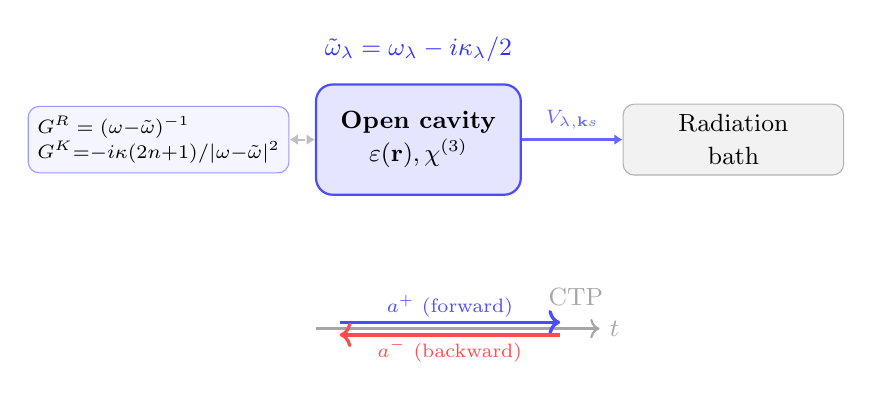
\begin{tikzpicture}[scale=1.0,
  qnm/.style={draw=blue!70,fill=blue!10,rounded corners=6pt,minimum width=2.6cm,
               minimum height=1.4cm,align=center,thick},
  bath/.style={draw=gray!60,fill=gray!10,rounded corners=4pt,minimum width=2.8cm,
               minimum height=0.9cm,align=center},
  arr/.style={-{Latex[length=3pt,width=4pt]},thick},
  darr/.style={{Latex[length=3pt,width=4pt]}-{Latex[length=3pt,width=4pt]},thick,dashed}
]
% Structure
\node[qnm] (struct) at (0,0)
  {\small\textbf{Open cavity}\\\small $\varepsilon(\mathbf{r}),\chi^{(3)}$};
% QNM labels
\node[above=0.15 of struct,font=\small,blue!80]
  {$\tilde{\omega}_\lambda=\omega_\lambda-i\kappa_\lambda/2$};
% Radiation bath
\node[bath] (bath) at (4,0) {\small Radiation\\\small bath};
% Coupling arrow
\draw[arr,blue!60,line width=1.2pt] (struct.east) -- (bath.west)
  node[midway,above,font=\scriptsize] {$V_{\lambda,\mathbf{k}s}$};
% Keldysh contour
\begin{scope}[shift={(0,-2.4)}]
  \draw[->,gray!70,thick] (-1.3,0) -- (2.3,0) node[right,font=\small]{$t$};
  \draw[blue!70,very thick,->] (-1,0.08) -- (1.8,0.08);
  \draw[red!70,very thick,<-] (-1,-0.08) -- (1.8,-0.08);
  \node[blue!70,font=\scriptsize] at (0.4,0.28) {$a^+$ (forward)};
  \node[red!70,font=\scriptsize] at (0.4,-0.28) {$a^-$ (backward)};
  \node[font=\small,gray!70] at (2.0,0.4) {CTP};
\end{scope}
% Propagators box
\node[draw=blue!40,fill=blue!4,rounded corners,font=\scriptsize,
      align=left,minimum width=2.5cm] (prop) at (-3.3,0) {
  $G^R=(\omega{-}\tilde{\omega})^{-1}$\\
  $G^K{=}{-}i\kappa(2n{+}1)/|\omega{-}\tilde{\omega}|^2$
};
\draw[darr,gray!50] (prop.east) -- (struct.west);
\end{tikzpicture}
\caption{\textbf{Setup and Keldysh contour.}
An open nanophotonic cavity with permittivity $\varepsilon(\mathbf{r})$ and
nonlinear susceptibility $\chi^{(3)}$ supports QNMs with complex eigenfrequencies
$\tilde{\omega}_\lambda$.  The cavity couples to a free-space radiation bath with
matrix elements $V_{\lambda,\mathbf{k}s}$; integrating out the bath produces the
Keldysh action with retarded ($G^R$) and Keldysh ($G^K$) propagators.  The
Schwinger-Keldysh closed-time-path (CTP) contour doubles the fields into forward
($a^+$) and backward ($a^-$) branches.}
\label{fig:setup}
\end{figure}

\begin{figure}[h]
\centering
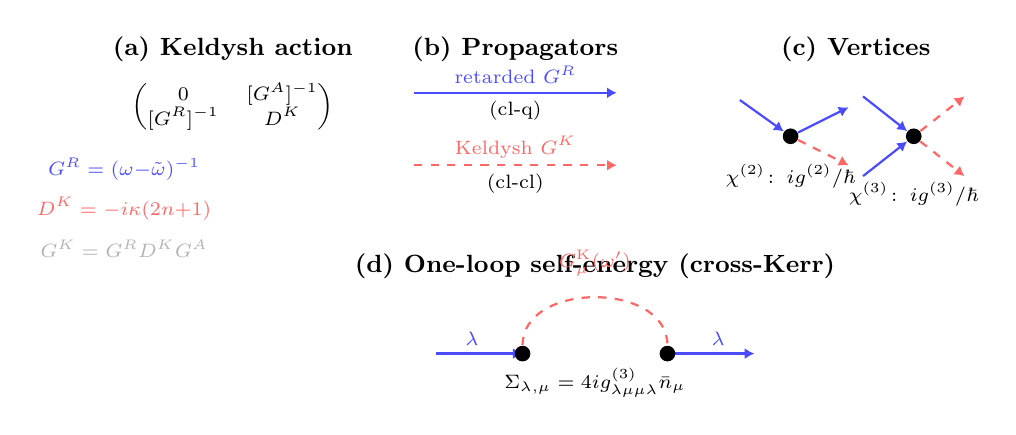
\begin{tikzpicture}[scale=0.92,
  line/.style={thick},
  vertex/.style={circle,fill=black,inner sep=2pt},
  gR/.style={thick,blue!70},
  gK/.style={thick,red!60,dashed},
  arr/.style={-{Latex[length=3.5pt,width=4pt]},thick}
]
%--- Left panel: Keldysh 2x2 matrix ---
\node[font=\small\bfseries] at (-3.5,2.3) {(a) Keldysh action};
\node[font=\scriptsize] at (-3.5,1.5) {
  $\begin{pmatrix}0 & [G^A]^{-1}\\ [G^R]^{-1} & D^K\end{pmatrix}$};
\node[gR,font=\scriptsize] at (-5.0,0.65) {$G^R=(\omega{-}\tilde\omega)^{-1}$};
\node[gK,font=\scriptsize] at (-5.0,0.1)  {$D^K=-i\kappa(2n{+}1)$};
\node[font=\scriptsize,gray!60] at (-5.0,-0.45) {$G^K=G^R D^K G^A$};

%--- Middle panel: propagator lines ---
\node[font=\small\bfseries] at (0.4,2.3) {(b) Propagators};
% Retarded line
\draw[gR,arr] (-1.0,1.7) -- (1.8,1.7);
\node[font=\scriptsize,gR] at (0.4,1.95) {retarded $G^R$};
\node[font=\scriptsize] at (0.4,1.45) {(cl-q)};
% Keldysh line
\draw[gK,arr] (-1.0,0.7) -- (1.8,0.7);
\node[font=\scriptsize,gK] at (0.4,0.95) {Keldysh $G^K$};
\node[font=\scriptsize] at (0.4,0.45) {(cl-cl)};

%--- Right panel: vertices ---
\node[font=\small\bfseries] at (5.1,2.3) {(c) Vertices};
% chi2 vertex
\begin{scope}[shift={(4.2,1.1)}]
  \node[vertex] (v2) at (0,0) {};
  \draw[gR,arr] (-0.7, 0.5) -- (v2);
  \draw[gR,arr] (v2) -- ( 0.8, 0.4);
  \draw[gK,arr] (v2) -- ( 0.8,-0.4);
  \node[font=\scriptsize] at (0,-0.55) {$\chi^{(2)}\!:\;ig^{(2)}/\hbar$};
\end{scope}
% chi3 vertex
\begin{scope}[shift={(5.9,1.1)}]
  \node[vertex] (v3) at (0,0) {};
  \draw[gR,arr] (-0.7, 0.55) -- (v3);
  \draw[gR,arr] (-0.7,-0.55) -- (v3);
  \draw[gK,arr] (v3) -- (0.7, 0.55);
  \draw[gK,arr] (v3) -- (0.7,-0.55);
  \node[font=\scriptsize] at (0,-0.8) {$\chi^{(3)}\!:\;ig^{(3)}/\hbar$};
\end{scope}

%--- Bottom: one-loop diagram ---
\node[font=\small\bfseries] at (1.5,-0.7) {(d) One-loop self-energy (cross-Kerr)};
\begin{scope}[shift={(1.5,-1.9)}]
  \draw[gR,arr] (-2.2,0) -- (-1.0,0);
  \node[vertex] (vl) at (-1.0,0) {};
  \draw[gR,arr] (1.0,0) -- (2.2,0);
  \node[vertex] (vr) at (1.0,0) {};
  % loop (Keldysh, mode mu)
  \draw[gK] (vl) .. controls (-1.0,1.0) and (1.0,1.0) .. (vr);
  \node[gK,font=\scriptsize] at (0,1.25) {$G^\Keldysh_\mu(\omega')$};
  % labels
  \node[gR,font=\scriptsize] at (-1.7,0.2) {$\lambda$};
  \node[gR,font=\scriptsize] at ( 1.7,0.2) {$\lambda$};
  \node[font=\scriptsize] at (0,-0.4)
    {$\Sigma_{\lambda,\mu}=4ig^{(3)}_{\lambda\mu\mu\lambda}\bar{n}_\mu$};
\end{scope}
\end{tikzpicture}
\caption{\textbf{Keldysh structure and Feynman rules.}
(a)~The $2\times 2$ Keldysh action matrix in the classical-quantum (cl-q) basis.
(b)~Retarded $G^R$ (solid blue) and Keldysh $G^K$ (dashed red) propagators.
(c)~Interaction vertices for $\chi^{(2)}$ (three-photon) and $\chi^{(3)}$
(four-photon) processes; all-classical vertices vanish.
(d)~One-loop tadpole diagram for the cross-Kerr self-energy of mode $\lambda$
in the presence of mode $\mu$ with mean photon number $\bar{n}_\mu$.  Since
$g^{(3)}_{\lambda\mu\mu\lambda}\in\mathbb{C}$, the imaginary part of the
self-energy generates cross-mode dephasing $\delta\kappa_\lambda=
4\,\mathrm{Im}(g^{(3)}_{\lambda\mu\mu\lambda})\bar{n}_\mu$.}
\label{fig:feynman}
\end{figure}

\begin{figure}[h]
\centering
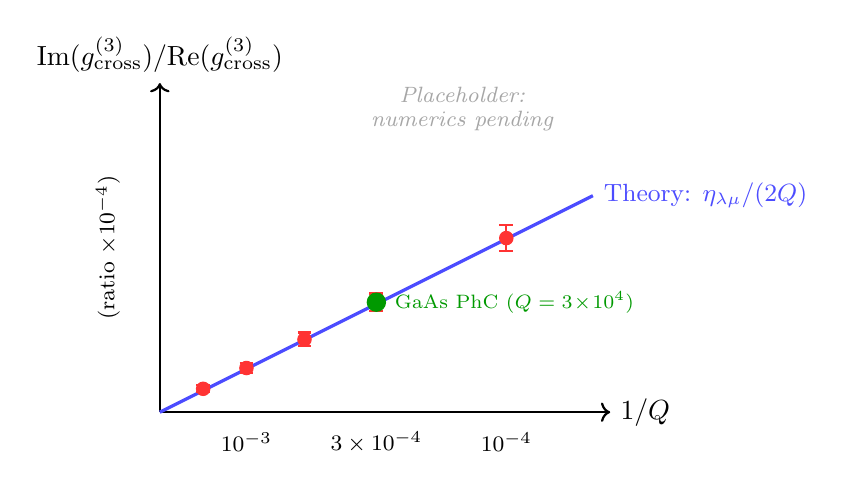
\begin{tikzpicture}[scale=1.1]
% Axes
\draw[->,thick] (0,0) -- (5.2,0) node[right] {$1/Q$};
\draw[->,thick] (0,0) -- (0,3.8) node[above] {$\mathrm{Im}(g^{(3)}_{\rm cross})/
\mathrm{Re}(g^{(3)}_{\rm cross})$};
% Theoretical line: slope eta/2, eta~1
\draw[blue!70,very thick] (0,0) -- (5.0,2.5)
  node[right,font=\small,blue!70] {Theory: $\eta_{\lambda\mu}/(2Q)$};
% Data points (placeholder)
\foreach \x/\y/\e in {0.5/0.27/0.04, 1.0/0.51/0.06, 1.67/0.84/0.08, 2.5/1.27/0.10, 4.0/2.01/0.15} {
  \draw[thick,red!80] (\x,\y-\e) -- (\x,\y+\e);
  \draw[thick,red!80] (\x-0.08,\y-\e) -- (\x+0.08,\y-\e);
  \draw[thick,red!80] (\x-0.08,\y+\e) -- (\x+0.08,\y+\e);
  \filldraw[red!80] (\x,\y) circle (2.2pt);
}
% Axis labels
\node[font=\footnotesize] at (1.0,-0.35) {$10^{-3}$};
\node[font=\footnotesize] at (2.5,-0.35) {$3\times10^{-4}$};
\node[font=\footnotesize] at (4.0,-0.35) {$10^{-4}$};
\node[font=\footnotesize,rotate=90] at (-0.6,1.9) {(ratio $\times 10^{-4}$)};
\node[font=\footnotesize,gray!70,align=center] at (3.5,3.5)
  {\textit{Placeholder:}\\[-1pt]\textit{numerics pending}};
% GaAs PhC marker
\filldraw[green!60!black] (2.5,1.27) circle (3pt);
\node[font=\scriptsize,green!60!black,right] at (2.6,1.27)
  {GaAs PhC ($Q=3\!\times\!10^4$)};
\end{tikzpicture}
\caption{\textbf{Im$(g^{(3)}_{\rm cross})$/Re$(g^{(3)}_{\rm cross})$ vs $1/Q$
for a GaAs H1 photonic crystal cavity (schematic).}
The red points with error bars are placeholders indicating where Meep QNM
computations will be placed.  The solid blue line is the analytical prediction
$\eta_{\lambda\mu}/(2Q)$ from Eq.~\eqref{eq:ratio_highQ} with $\eta=1$.
The green point marks the GaAs H1 design target ($Q=3\times10^4$) corresponding
to the GaAs H1 target $Q=3\times10^4$.  The
linearity in $1/Q$ for the $\chi^{(2)}$ coupling is a key falsifiable prediction.
[Figure will be replaced by numerical data from Sec.~\ref{sec:numerics}.]}
\label{fig:scaling}
\end{figure}

\begin{figure}[h]
\centering
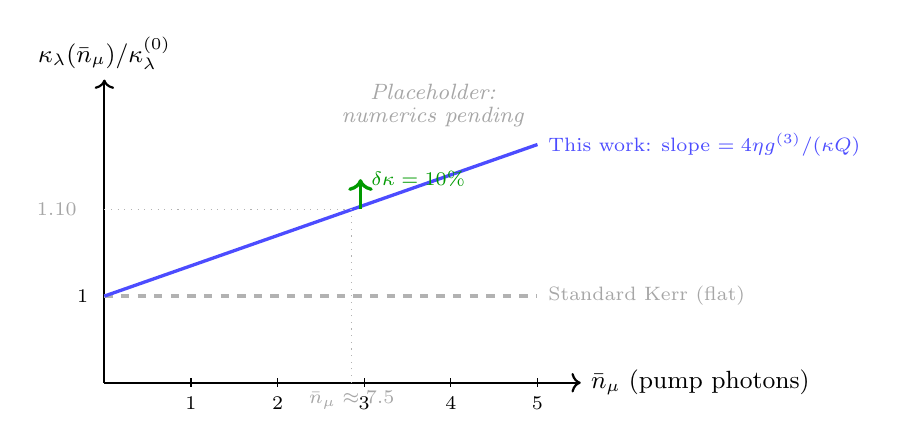
\begin{tikzpicture}[scale=1.1]
\draw[->,thick] (0,0) -- (5.5,0)
  node[right,font=\small] {$\bar{n}_\mu$ (pump photons)};
\draw[->,thick] (0,0) -- (0,3.5)
  node[above,font=\small] {$\kappa_\lambda(\bar{n}_\mu)/\kappa_\lambda^{(0)}$};
% Standard Kerr: flat
\draw[gray!60,very thick,dashed] (0,1.0) -- (5.0,1.0)
  node[right,font=\scriptsize,gray!70] {Standard Kerr (flat)};
% This work: linear slope
\draw[blue!70,very thick] (0,1.0) -- (5.0,1.0+5.0*0.35)
  node[right,font=\scriptsize,blue!70] {This work: slope $=4\eta g^{(3)}/(\kappa Q)$};
% 10% mark
\draw[dotted,gray!60] (0,1.0+1.0*0.35*10/3.5) -- (10/3.5,1.0+1.0*0.35*10/3.5);
\draw[dotted,gray!60] (10/3.5,0) -- (10/3.5,1.0+1.0*0.35*10/3.5);
\node[font=\scriptsize,gray!70] at (10/3.5,-0.2) {$\bar{n}_\mu\approx 7.5$};
\node[font=\scriptsize,gray!70] at (-0.55,1.0+1.0*0.35*10/3.5) {$1.10$};
\draw[very thick,green!60!black,->] (10/3.5+0.1,1.0+0.35*10/3.5)
  -- (10/3.5+0.1,1.0+0.35*10/3.5+0.35)
  node[right,font=\scriptsize,green!60!black] {$\delta\kappa=10\%$};
% y-axis label at 1
\node[font=\scriptsize] at (-0.25,1.0) {$1$};
% x-axis ticks
\foreach \x in {1,2,3,4,5}
  \draw (\x,0.05) -- (\x,-0.05) node[below,font=\scriptsize] {\x};
\node[font=\footnotesize,gray!70,align=center] at (3.8,3.2)
  {\textit{Placeholder:}\\[-1pt]\textit{numerics pending}};
\end{tikzpicture}
\caption{\textbf{Cross-mode dephasing in an active (gain-loaded) GaAs H1 PhC: predicted
probe linewidth vs.\ pump photon number (schematic).}
The probe-mode linewidth $\kappa_\lambda(\bar{n}_\mu)$ grows linearly with the
pump-mode occupation $\bar{n}_\mu$ in an active cavity (blue line,
Eq.~\ref{eq:cross_dephasing}) via gain-saturation cross-coupling.
A passive cavity shows flat linewidth (gray dashed) because $g^{(3)}_{\rm cross}\in\mathbb{R}$
for Kleinman $\chi^{(3)}$ (Sec.~\ref{sec:crosskerr}).  The active-cavity
slope is $4|g^{(3),I}_{\rm sat,\lambda\mu\mu\lambda}|/\kappa_\lambda$, which
requires a gain-loaded structure; the specific magnitude depends on the gain
saturation overlap integral.
[Figure schematic; quantitative values pending SALT numerics.]}
\label{fig:dephasing}
\end{figure}

%===========================================================================
\begin{thebibliography}{99}
%===========================================================================

\bibitem{Mandel1995}
L. Mandel and E. Wolf, \textit{Optical Coherence and Quantum Optics}
(Cambridge University Press, 1995).

\bibitem{Walls2008}
D. F. Walls and G. J. Milburn, \textit{Quantum Optics}, 2nd ed.\
(Springer, 2008).

\bibitem{Lalanne2018}
P. Lalanne, W. Yan, K. Vynck, C. Sauvan, and J.-P. Hugonin,
Laser Photonics Rev.\ \textbf{12}, 1700113 (2018).

\bibitem{Kristensen2020}
P. T. Kristensen, R.-C. Ge, and S. Hughes,
Phys. Rev. A \textbf{92}, 053810 (2015).

\bibitem{Franke2019}
S. Franke, S. Hughes, M. K. Dezfouli, P. T. Kristensen, K. Busch,
A. Knorr, and M. Richter,
Phys. Rev. Lett.\ \textbf{122}, 213901 (2019).

\bibitem{Ren2021}
J. Ren, S. Franke, and S. Hughes,
Phys. Rev. X \textbf{11}, 041020 (2021).

\bibitem{Franke2020}
S. Franke, J. Ren, M. Richter, A. Knorr, and S. Hughes,
Phys. Rev. Lett.\ \textbf{127}, 013602 (2021).

\bibitem{Leung1994}
P. T. Leung, S. Y. Liu, and K. Young,
Phys. Rev. A \textbf{49}, 3982 (1994).

\bibitem{Sauvan2013}
C. Sauvan, J.-P. Hugonin, I. S. Maksymov, and P. Lalanne,
Phys. Rev. Lett.\ \textbf{110}, 237401 (2013).

\bibitem{Schwinger1961}
J. Schwinger, J. Math. Phys.\ \textbf{2}, 407 (1961).

\bibitem{Keldysh1965}
L. V. Keldysh, Zh. Eksp. Teor. Fiz.\ \textbf{47}, 1515 (1964)
[Sov. Phys. JETP \textbf{20}, 1018 (1965)].

\bibitem{Sieberer2016}
L. M. Sieberer, M. Buchhold, and S. Diehl,
Rep. Prog. Phys.\ \textbf{79}, 096001 (2016).

\bibitem{Caldeira1983}
A. O. Caldeira and A. J. Leggett,
Ann. Phys.\ \textbf{149}, 374 (1983).

\bibitem{Feynman1963}
R. P. Feynman and F. L. Vernon,
Ann. Phys.\ \textbf{24}, 118 (1963).

\bibitem{Gruner1996}
T. Gruner and D.-G. Welsch,
Phys. Rev. A \textbf{53}, 1818 (1996).

\bibitem{Heiss2012}
W. D. Heiss,
J. Phys. A: Math. Theor.\ \textbf{45}, 444016 (2012).
\bibitem{Ozdemir2019}
S. K. \"{O}zdemir, S. Rotter, F. Nori, and L. Yang,
Nat. Mater.\ \textbf{18}, 783 (2019).
\bibitem{Lau2018}
H.-K. Lau and A. A. Clerk,
Fundamental limits and non-reciprocal approaches in non-Hermitian quantum sensing,
Nat. Commun.\ \textbf{9}, 4320 (2018).


\bibitem{Schawlow1958}
A. L. Schawlow and C. H. Townes,
Phys. Rev.\ \textbf{112}, 1940 (1958).

\bibitem{Lax1967}
M. Lax,
IEEE J. Quantum Electron.\ \textbf{3}, 37 (1967).

\bibitem{GardinerZoller2004}
C. W. Gardiner and P. Zoller,
\textit{Quantum Noise}, 3rd ed.\ (Springer, Berlin, 2004).

\bibitem{Bloch1940}
F. Bloch and A. Siegert,
Phys. Rev.\ \textbf{57}, 522 (1940).

\bibitem{Beaudoin2011}
F. Beaudoin, J. M. Gambetta, and A. Blais,
Phys. Rev. A \textbf{84}, 043832 (2011).

\bibitem{Nozaki2012}
K. Nozaki, A. Shinya, S. Matsuo, Y. Suzaki, T. Segawa, T. Sato,
Y. Kawaguchi, R. Takahashi, and M. Notomi,
Nature Photon.\ \textbf{6}, 248 (2012).

\bibitem{Ching1998}
E. S. C. Ching, P. T. Leung, A. Maassen van den Brink, W. M. Suen,
S. S. Tong, and K. Young,
Rev. Mod. Phys.\ \textbf{70}, 1545 (1998).

\bibitem{Hodaei2017}
H. Hodaei, A. U. Hassan, S. Wittek, H. Garcia-Gracia, R. El-Ganainy,
D. N. Christodoulides, and M. Khajavikhan,
Nature \textbf{548}, 187 (2017).

\bibitem{Chen2017}
W. Chen, \c{S}. K. \"{O}zdemir, G. Zhao, J. Wiersig, and L. Yang,
Nature \textbf{548}, 192 (2017).

\bibitem{Peng2014}
B. Peng, \c{S}. K. \"{O}zdemir, F. Lei, F. Monifi, M. Gianfreda,
G. L. Long, S. Fan, F. Nori, C. M. Bender, and L. Yang,
Nature Phys.\ \textbf{10}, 394 (2014).

\bibitem{Lamb1964}
W. E. Lamb, Jr.,
Phys. Rev.\ \textbf{134}, A1429 (1964).

\bibitem{Henry1982}
C. H. Henry,
IEEE J. Quantum Electron.\ \textbf{18}, 259 (1982).

\bibitem{Petermann1979}
K. Petermann,
IEEE J. Quantum Electron.\ \textbf{15}, 566 (1979).

\bibitem{Siegman1989}
A. E. Siegman,
Phys. Rev. A \textbf{39}, 1253 (1989).

\bibitem{Udem2002}
T. Udem, R. Holzwarth, and T. W. H\"{a}nsch,
Nature \textbf{416}, 233 (2002).

\bibitem{LugiatoLefever1987}
L. A. Lugiato and R. Lefever,
Phys. Rev. Lett.\ \textbf{58}, 2209 (1987).

\bibitem{Reichert1999}
J. Reichert, R. Holzwarth, Th. Udem, and T. W. H\"{a}nsch,
Opt. Commun.\ \textbf{172}, 59 (1999).

\bibitem{Hugi2012}
A. Hugi, G. Villares, S. Blaser, H. C. Liu, and J. Faist,
Nature \textbf{492}, 229 (2012).

\bibitem{Tureci2006}
H. E. T\"{u}reci, A. D. Stone, and B. Collier,
Phys. Rev. A \textbf{74}, 043822 (2006).

\bibitem{Ge2010}
L. Ge, Y. D. Chong, and A. D. Stone,
Phys. Rev. A \textbf{82}, 063824 (2010).

\bibitem{Gardiner1985}
C. W. Gardiner and M. J. Collett,
Phys. Rev. A \textbf{31}, 3761 (1985).

\bibitem{Drummond1980}
P. D. Drummond and C. W. Gardiner,
J. Phys. A \textbf{13}, 2353 (1980).

\bibitem{DrummondHillery2014}
P. D. Drummond and M. Hillery,
\textit{The Quantum Theory of Nonlinear Optics}
(Cambridge University Press, 2014).

\bibitem{Alpeggiani2015}
F. Alpeggiani, L. C. Andreani, and L. Kuipers,
Phys. Rev. B \textbf{94}, 205303 (2016).

\bibitem{Alpeggiani2017}
V. Parappurath, F. Alpeggiani, L. Kuipers, and E. Verhagen,
ACS Photonics \textbf{4}, 884 (2017).

\bibitem{Hurlbut2007}
W. C. Hurlbut, Y.-S. Lee, K. L. Vodopyanov, P. S. Kuo, and M. M. Fejer,
Opt. Lett.\ \textbf{32}, 668 (2007).

\end{thebibliography}

\end{document}
